\chapter{Первоначальные химические понятия}

\section{Знакомство с химической связью}\label{sec:introduction_to_chemical_bonding}

\begin{wrapfigure}{l}{0.4\textwidth}
    \centering
    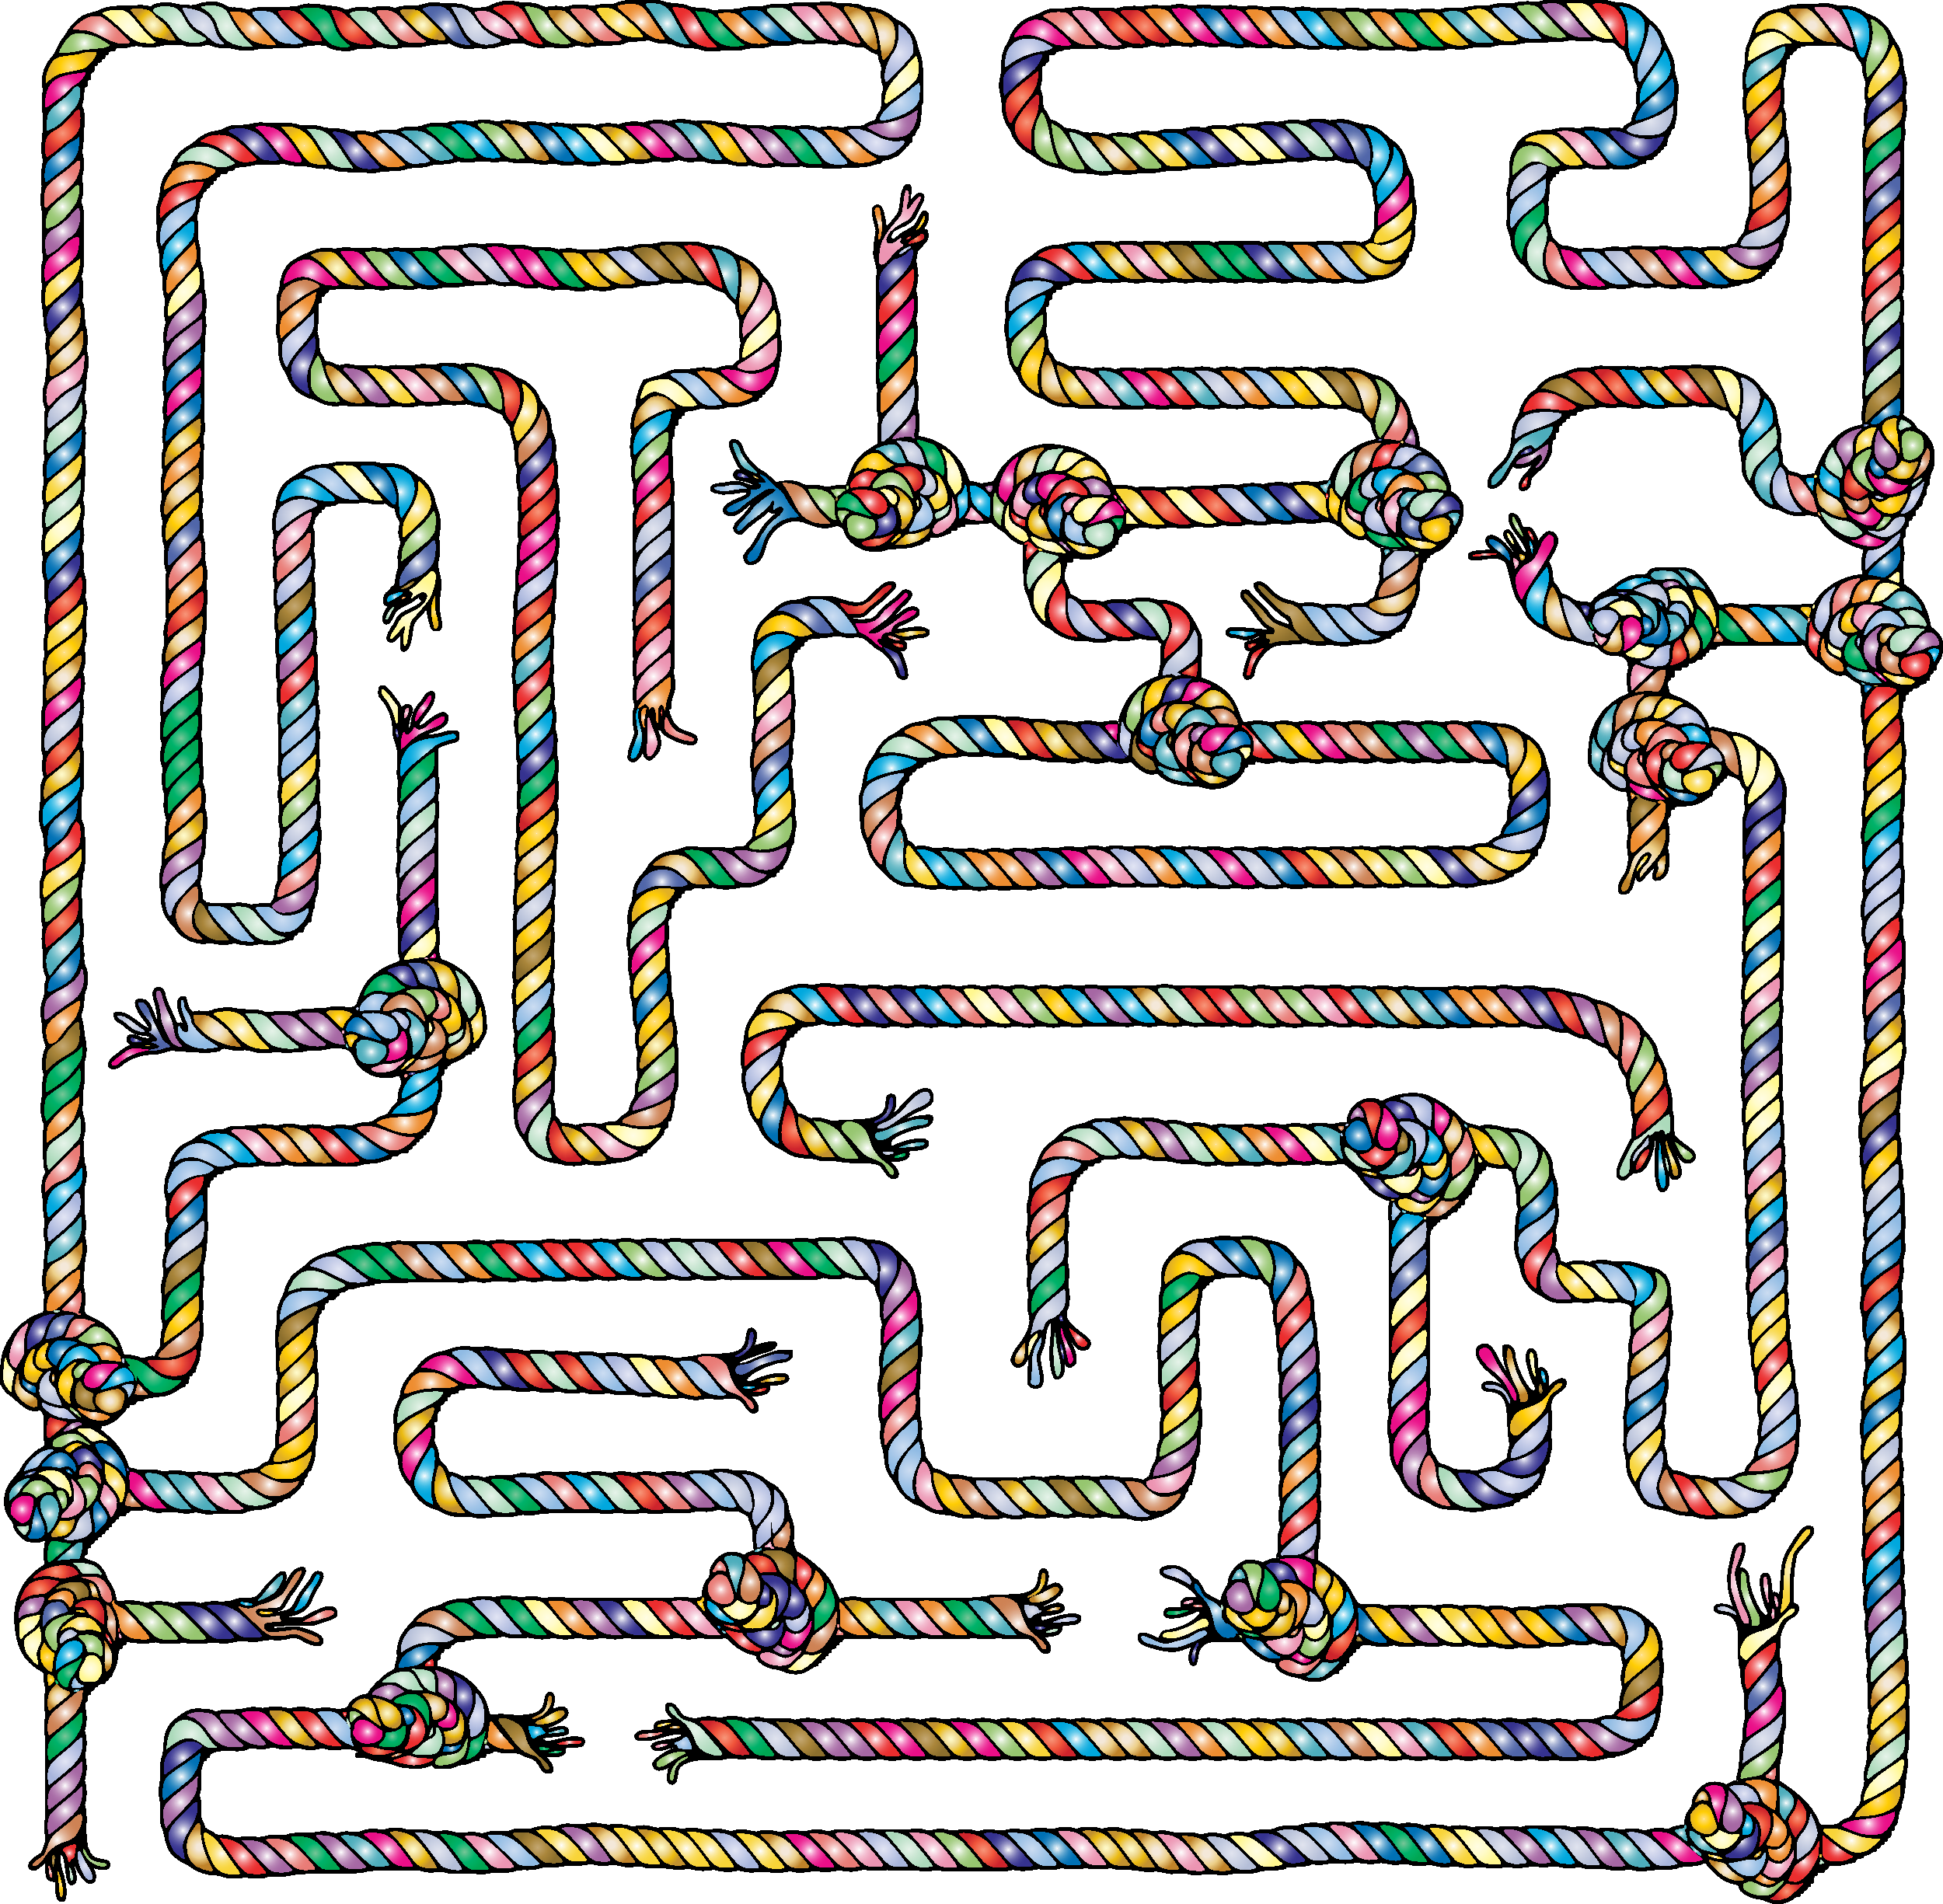
\includegraphics[width=5cm]{figs/introduction_to_chemical_bonding/ropes.pdf}
\end{wrapfigure}

\hspace*{\parindent}Соединения состоят из атомов \hyperref[term:chemical_element]{химических элементов}, соединённых \hyperref[term:chemical_bond]{химической связью}. Большинству атомов выгодно образовывать химические связи, иначе никаких химических соединений в природе бы не существовало. При образовании связи атомы стремятся изменить свои электронные оболочки до более устойчивых конфигураций, чтобы достичь состояния с минимальной возможной энергией. Это можно сделать двумя способами:

\begin{itemize}
    \item дозаполнить атомные орбитали электронами;
    \item опустошить свои атомные орбитали.
\end{itemize}

Но где взять электроны для заполнения оболочек или куда их отдавать? Для этого атомы используют электроны и атомные орбитали \emph{другого атома} с подходящей электронной конфигурацией.

Перераспределение электронной плотности при этом заставляет атомы находиться рядом, чтобы реализовать взаимодействие их электронных оболочек и снизить энергию~--- такое явление и называют \emph{химической связью}. В этом разделе мы познакомимся с основными типами химической связи.

\subsection*{Ковалентная неполярная связь}

Химическая связь реализуется при помощи \emph{двух электронов}, которые начинают занимать новую орбиталь, образующуюся из исходных атомных орбиталей атомов, образующих связь. Эта новая орбиталь называется \emph{молекулярной орбиталью} (МО) и является общей для обоих атомов.

При взаимодействии АО атомов образуются две молекулярные орбитали (сколько АО смешивается, столько МО и образуется), однако вторая МО оказывается выше по энергии и остаётся пустой.

Например, атом фтора имеет один неспаренный электрон на 2p-орбитали, который может участвовать в формировании связи с другим атомом фтора с образованием молекулы \ce{F2} (рис.~\ref{fig:fluorine_molecular_orbitals}).

\begin{figure}[htbp]
    \centering
    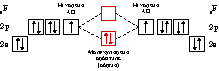
\includegraphics[width=10cm]{figs/introduction_to_chemical_bonding/fluorine_molecular_orbitals.pdf}
    \caption{Молекулярные орбитали молекулы фтора.}
    \label{fig:fluorine_molecular_orbitals}
\end{figure}

Такой тип связи называется \textbf{ковалентной неполярной связью}\label{term:non-polar_covalent_bond}\index{ковалентная неполярная связь}, подразумевая, что связывающая электронная плотность в равной мере принадлежит обоим атомам. Ковалентные неполярные связи образуют между собой атомы одного химического элемента или атомы с очень близкой электроотрицательностью (например, связь \ce{C\bond{1}H}).

Иногда химическую связь показывают не чертой, как это обычно делают в \hyperref[term:planar_structural_formula]{структурных формулах}, а указывая электроны на внешней оболочке атома в виде точек (рис.~\ref{fig:electrons_as_points}). 

При этом показывают электронную пару, образующую связь, как общую для двух атомов. Электроны полностью заполненных орбиталей изображают как \textbf{неподелённые электронные пары}\label{term:lone_electron_pairs}\index{неподелённая электронная пара} (НЭП) с оставшихся сторон символа атома.

Например, фтор имеет на внешней оболочке три НЭП и один неспаренный электрон, который и участвует в образовании связи.

\begin{figure}[htbp]
    \centering
    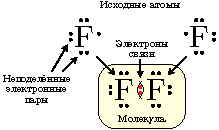
\includegraphics[width=6cm]{figs/introduction_to_chemical_bonding/electrons_as_points.pdf}
    \caption{Изображение электронов на внешней оболочке атома в виде точек.}
    \label{fig:electrons_as_points}
\end{figure}

Между двумя атомами могут образовываться и несколько связей (двойная, тройная). Такие связи называют \emph{кратными связями}. Каждая из таких связей тоже образуется при помощи пары электронов.

Например, у кислорода имеется два неспаренных электрона на 2p-орбиталях, которые он может использовать для образования \emph{двойной связи} с другим атомом кислорода (рис.~\ref{fig:oxygen_molecular_orbitals})\footnote{На самом деле в молекуле кислорода более сложная структура связи, об этом мы поговорим в главе, посвящённой углубленному изучению химической связи.}.

\begin{figure}[htbp]
    \centering
    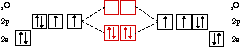
\includegraphics[width=10cm]{figs/introduction_to_chemical_bonding/oxygen_molecular_orbitals.pdf}
    \caption{Молекулярные орбитали молекулы кислорода.}
    \label{fig:oxygen_molecular_orbitals}
\end{figure}

\subsection*{Ковалентная полярная связь}

А что будет, если химическую связь образуют атомы, имеющие разные энергии орбиталей? Энергии высших занятых атомных орбиталей понижаются в периодической таблице слева направо (в периоде) и повышаются сверху вниз (в группе). К примеру, энергия 3s-орбитали атома натрия лежит выше, чем 3p-орбитали атома хлора, а 3p-орбиталь хлора выше по энергии, чем 2p-орбиталь фтора.

При образовании связи при помощи орбиталей разных энергий та молекулярная орбиталь, которая лежит ниже и заселена электронами становится больше похожа (по форме и расположению электронной плотности) на АО с более низкой энергией. Другими словами, электроны связи больше времени проводят возле атома, который предоставил АО с более низкой энергией.

Например, в молекуле фтороводорода молекулярная орбиталь, заселённая электронами ближе по энергии и больше похожа на p-орбиталь атома фтора (рис.~\ref{fig:HF_molecular_orbitals}).

\begin{figure}[htbp]
    \centering
    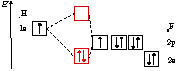
\includegraphics[width=8cm]{figs/introduction_to_chemical_bonding/HF_molecular_orbitals.pdf}
    \caption{Молекулярные орбитали молекулы \ce{HF}.}
    \label{fig:HF_molecular_orbitals}
\end{figure}

Таким образом, электронная плотность несколько смещается в сторону атома с более низкой энергией АО, образующей связь. Такой тип связи называется \textbf{ковалентной полярной связью}\label{term:polar_covalent_bond}\index{ковалентная полярная связь}. Такие связи образуют между собой элементы, не слишком далеко расположенные друг от друга в периодах, потому что в этом случае энергии их орбиталей различаются по энергии, но не очень сильно.

\subsection*{Ионная связь}

Для элементов, АО которых \emph{сильно отличаются по энергии}, например, элементов, лежащих в начале и в конце периодов характерен \textbf{ионный тип связи}\label{term:ionic_bond}\index{ионная связь}.

В случае ионной связи занятая электронами молекулярная орбиталь становится настолько похожа на более низколежащую АО, что становится практически неотличима от неё, как, например, во фториде лития (рис.~\ref{fig:LiF_molecular_orbitals}).

\begin{figure}[htbp]
    \centering
    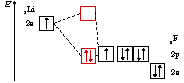
\includegraphics[width=8cm]{figs/introduction_to_chemical_bonding/LiF_molecular_orbitals.pdf}
    \caption{Молекулярные орбитали фторида лития.}
    \label{fig:LiF_molecular_orbitals}
\end{figure}

В таком случае считают, что происходит \emph{полная передача электрона} на АО с низкой энергией, а атомы, образующие связь, превращаются в ионы. В данном случае фтор полностью достраивает свою электронную оболочку до конфигурации атома неона, превращаясь в анион \ce{F^-}, а литий приобретает электронную конфигурацию атома гелия, превращаясь в катион \ce{Li^+} (рис.~\ref{fig:LiF_molecular_orbitals_var_2}).

\begin{figure}[htbp]
    \centering
    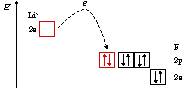
\includegraphics[width=8cm]{figs/introduction_to_chemical_bonding/LiF_molecular_orbitals_2_var.pdf}
    \caption{Образование ионов при ионном типе связи.}
    \label{fig:LiF_molecular_orbitals_var_2}
\end{figure}

\subsection*{Донорно-акцепторная связь}

В приведённых выше типах связи каждый атом предоставлял для её образования по одному электрону. Однако ничего не мешает образовать связь, используя полностью пустую АО одного атома и полностью заполненную орбиталь другого атома.

В этом случае связь также образуется парой электронов, но они оба изначально принадлежат одному из атомов. Такой тип связи называется \textbf{донорно-акцепторной связью}\label{term:coordinate_covalent_bond}\index{донорно-акцепторная связь}.

Например, такая связь имеется в ионе аммония (рис.~\ref{fig:ammonium_ion}), где азот образует четыре связи, несмотря на то, что имеет всего три неспаренных электрона (на 2p-подуровне).

\begin{figure}[htbp]
    \centering
    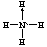
\includegraphics[width=2cm]{figs/introduction_to_chemical_bonding/ammonium_ion.pdf}
    \caption{Связи в ионе аммония. Донорно-акцепторная связь показана стрелкой.}
    \label{fig:ammonium_ion}
\end{figure}

Четвёртую связь азот образует по донорно-акцепторному механизму, предоставляя электроны полностью занятой орбитали (рис.~\ref{fig:coordinate_covalent_bond}), которые размещаются на вакантной 1s-орбитали атома водорода.

\begin{figure}[htbp]
    \centering
    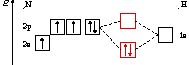
\includegraphics[width=8cm]{figs/introduction_to_chemical_bonding/coordinate_covalent_bond.pdf}
    \caption{Образование донорно-акцепторной связи в ионе аммония.}
    \label{fig:coordinate_covalent_bond}
\end{figure}

Атом, который предоставляет электронную пару (в нашем примере~--- азот), называется \emph{донором}, его записывают, добавляя ему положительный заряд, который символизирует то, что он предоставил для образования связи два электрона вместо одного.

Атом, который предоставил пустую атомную орбиталь (водород), называют \emph{акцептором}. Ему приписывают отрицательный заряд, если он изначально был нейтральным, показывая, что он образовал связь с другим атомом, не отдавая свой электрон. Однако в случае иона аммония водород уже приходит в виде иона \ce{H^+}, поэтому суммарный положительный заряд приписывают атому азота.

При изображении донорно-акцепторной связи в структурной формуле соединения связь нужно показать направленной стрелкой от донора к акцептору вместо обычной черты, как показано на рис.~\ref{fig:ammonium_ion}.

\subsection*{Металлическая связь}

В металлах внешние электроны слабо связаны с атомным ядром и достаточно подвижны для того, чтобы перемещаться от связи к связи, именно поэтому металлы так хорошо проводят электрический ток.

По той же причине слои атомов металлов довольно легко смещаются друг относительно друга, обеспечивая пластичность металлов как материала.

В целом связи, образованные в металлах, имеют \textbf{металлический тип связи}\label{term:metallic_bond}\index{металлическая связь}, этот тип связи мы подробнее изучим в следующих уроках.

Сформулируйте термины, представленные ниже, а затем переходите к решению задач.

\begin{termlist}
    \hyperref[term:non-polar_covalent_bond]{Ковалентная неполярная связь}, 
    \hyperref[term:lone_electron_pairs]{неподелённая электронная пара},
    \hyperref[term:polar_covalent_bond]{ковалентная полярная связь},
    \hyperref[term:ionic_bond]{ионная связь},
    \hyperref[term:coordinate_covalent_bond]{донорно-акцепторная связь}.
\end{termlist}

\begin{problem}{}{introduction_to_chemical_bonding1}
    В следующих веществах определите тип связи.
    \begin{enumerate}[label=\arabic*)]
        \item Металлический натрий;
        \item \ce{NaCl};
        \item \ce{N2};
        \item \ce{SiC};
        \item \ce{H2O}.
    \end{enumerate}
    \begin{sol}{\ref{prob:introduction_to_chemical_bonding1}}
        Типы связей следующие:
        \begin{enumerate}[label=\arabic*)]
        \item металлическая;
        \item ионная;
        \item ковалентная неполярная;
        \item ковалентная полярная;
        \item ковалентная полярная.
    \end{enumerate}
    \end{sol}
\end{problem}

\clearpage

\section{Электроотрицательность}\label{sec:electronegativity}

\hspace*{\parindent}Как стало понятно из описания \hyperref[sec:introduction_to_chemical_bonding]{процесса образования химических связей}, атомы различных химических элементов обладают разной способностью удерживать возле себя электроны, что приводит к смещению электронной плотности связи, если она образована различными элементами, и даже изменению характера связи (ковалентная полярная $\to$ ионная).

К количественной оценке способности атомов удерживать электроны пришли следующим образом. При изучении химической связи \ce{A-B}, образованной разными химическими элементами, американский учёный Лайнус Полинг обнаружил, что энергия такой связи выше, чем среднее значение энергий связей \ce{A-A} и \ce{B-B}.

\textbf{Энергией связи}\label{term:bond_energy}\index{энергия связи} (или энергией диссоциации связи) называют энергию, которую необходимо затратить, чтобы разорвать связь, то есть разъединить атомы на бесконечно далёкое расстояние. Измеряют энергию связи в \unit{\kJ\per\mole} или \unit{\eV}.

Полинг предположил следующее. При образовании связей в таких молекулах из-за различного заряда ядра атомов и электронного строения атомы одного химического элемента обладают большей способностью удерживать возле себя электроны, смещая электронную плотность связи в свою сторону. Из-за такого смещения на атомах возникают частичные заряды $\delta^{+}$ и $\delta^{-}$, меньше заряда электрона $e$, равные по величине и противоположные по знаку, например:

\begin{equation*}
    \ce{\overset{\delta+}{\text{H}}\bond{->}\overset{\delta-}{\text{F}}}.
\end{equation*}

Стрелочкой показано направление смещения электронной плотности относительно середины связи.

Электростатическое взаимодействие двух разноимённых зарядов приводит к дополнительной стабилизации связи и увеличивает её энергию. Величина этой дополнительной энергии связи и определяется взаимной способностью элементов (участвующих в образовании связи) удерживать возле себя электроны химической связи. Эта способность получила название \textbf{электроотрицательность}\label{term:electronegativity}\index{электроотрицательность} (ЭО) химического элемента.

Электроотрицательность обозначается буквой $\chi$ (читается <<хи>>).

\subsection*{Электроотрицательность по Полингу}

Существует несколько шкал электроотрицательностей. Самая известная шкала~--- \textbf{электроотрицательность по Полингу}\label{term:Pauling_electronegativity}\index{электроотрицательность по Полингу}. В ней разность электроотрицательностей для элементов по определению равна:

\begin{equation*}
    |\chi_A - \chi_B| = (\text{eV})^{-\frac{1}{2}} \sqrt{E_d(\text{AB}) - \frac{E_d(\text{AA}) + E_d(\text{BB})}{2}}.
\end{equation*}

где $E_d$~--- энергия диссоциации связей в единицах \unit{\eV}, а коэффициент $(\text{eV})^{-\frac{1}{2}}$ включён для того, чтобы результат был безразмерным.

Поскольку зная величины энергий связи можно рассчитать только разницу, но не сами величины $\chi$, то необходимо принять значение для какого-то элемента в качестве точки отсчёта. В шкале Полинга это фтор: ему было присвоено значение \num{4,0}. При этом также удалось избежать отрицательных значений для других элементов.

Величины электроотрицательностей по Полингу для тех элементов, для которых она определялась, приведены в приложении~\ref{appendix:electronegativity}.

\subsection*{Электроотрицательность по Малликену}

Американский учёный Роберт Малликен решил рассмотреть электроотрицательность как абсолютную, а не относительную величину. Он рассуждал так: способность атома удерживать электроны определяется его граничными орбиталями~--- ВЗАО и НСАО. Чем ниже по энергии верхняя занятая атомная орбиталь, тем труднее оторвать электрон от исходного атома.

Если же электрон попадает на нижнюю свободную атомную орбиталь атома, то выигрыш в энергии тем больше, чем ниже расположена НСАО, поскольку тем труднее будет удалить этот электрон из атома обратно.

\begin{figure}
    \centering
    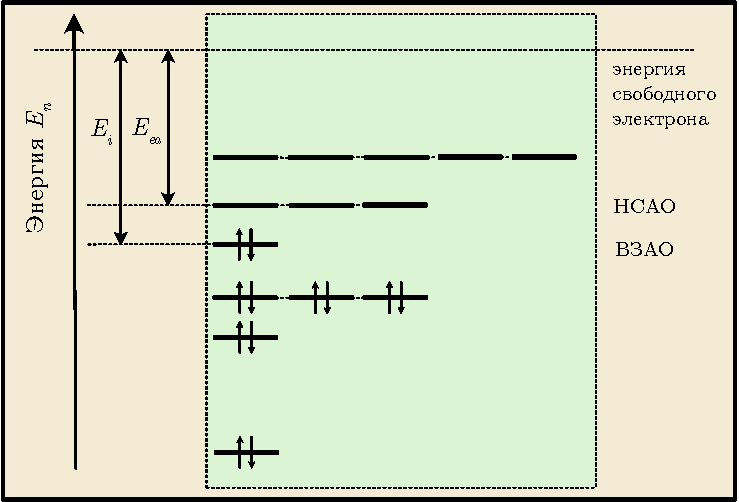
\includegraphics[width=10cm]{figs/electronegativity/mulliken_electronegativity.pdf}
    \caption{Потенциал ионизации и сродство к электрону.}
    \label{fig:ionization_energy_and_electron_affinity}
\end{figure}

\textbf{Потенциал ионизации}\label{term:ionization_energy}\index{потенциал ионизации} $E_i$~--- это энергия, необходимая для того, чтобы удалить электрон с верхней занятой орбитали (рис.~\ref{fig:ionization_energy_and_electron_affinity}).

\textbf{Сродство к электрону}\label{term:electron_affinity}\index{сродство к электрону} $E_{ea}$~--- это энергия, которая выделяется при добавлении электрона на нижнюю свободную атомную орбиталь атома.

\textbf{Электроотрицательность по Малликену}\label{term:Mulliken_electronegativity}\index{электроотрицательность по Малликену}~--- это среднее арифметическое потенциала ионизации и сродства к электрону:

\begin{equation*}
    \chi = \frac{E_i + E_{ea}}{2}.
\end{equation*}

ЭО по Малликену измеряется в \unit{\kJ\per\mole} или электрон-вольтах. Шкалы Полинга и Малликена (и, кстати, другие существующие шкалы) довольно хорошо согласуются друг с другом (в плане последовательности элементов).

\subsection*{Критерий ионности связи}

Электроотрицательность позволяет нам примерно оценить, какой тип связи будут образовывать химические элементы друг с другом. Для этого нам нужно подсчитать \emph{разность электроотрицательностей} элементов. Формально принято считать, что элементы образуют ковалентную связь до тех пор, пока разность ЭО между ними $\Delta \chi < \num{1,7}$ по шкале Полинга. Если $\Delta \chi > \num{1,7}$, то считается, что атомы образуют ионный тип связи. При этом нужно помнить о следующих моментах.

\begin{itemize}
    \item Полностью ионной связи не существует. Любая ионная связь обладает определённой долей ковалентности, или, проще говоря, электронная плотность никогда полностью не смещена к одному из атомов. Чёткой границы между ковалентной полярной и ионной связью нет. Можно даже представлять ионную связь как \emph{очень полярную ковалентную связь}.
    \item Тип связи зависит не только от самих атомов, образующих связь, но и от \emph{соседних атомов, связанных с ними}. Дело в том, что эти атомы сами способны оттягивать на себя или предоставлять электронную плотность, изменяя электроотрицательность атомов рассматриваемой связи.
    \item В таблице электроотрицательностей указаны значения для \emph{нейтральных атомов}. Для атомов, находящихся в состоянии \emph{ионов}, эти значения использовать нельзя. 
\end{itemize}

Повторите термины, изученные в этом разделе, и проверьте своё понимание материала, решив несколько задач.

\begin{termlist}
    \hyperref[term:bond_energy]{Энергия связи}, 
    \hyperref[term:electronegativity]{электроотрицательность},
    \hyperref[term:Pauling_electronegativity]{электроотрицательность по Полингу}, 
    \hyperref[term:ionization_energy]{потенциал ионизации}, 
    \hyperref[term:electron_affinity]{сродство к электрону}, 
    \hyperref[term:Mulliken_electronegativity]{электроотрицательность по Малликену}.
\end{termlist}

\begin{problem}{}{electronegativity1}
    Какие химические элементы имеют наибольшую и наименьшую электроотрицательность? Как изменяется электроотрицательность в периодической таблице и почему?

    \begin{sol}{\ref{prob:electronegativity1}}
        Фтор имеет наибольшую, а цезий и франций~--- наименьшую электроотрицательности.
        \medskip
        В периодах ЭО растёт, так как увеличивается заряд ядра атома и орбитали поджимаются к ядру. В группах ЭО уменьшается, поскольку происходит последовательное заполнение оболочек, расположенных всё дальше от ядра.
    \end{sol}
\end{problem}

\begin{problem}{}{electronegativity2}
    Как вы считаете, можно ли считать электроотрицательность химического элемента постоянной величиной? Почему?

    \begin{sol}{\ref{prob:electronegativity2}}
        Электроотрицательность зависит от уровней энергии ВЗАО и НСАО, которые могут меняться, например, при образовании ионов из нейтрального атома. В этом случае ВЗАО и НСАО становятся другие атомные орбитали, лежащие ниже или выше. Поэтому электроотрицательность нельзя считать постоянной величиной.
    \end{sol}
\end{problem}

\begin{problem}{}{electronegativity3}
    Может ли ковалентная полярная связь наблюдаться между двумя одинаковыми атомами?

    \begin{sol}{\ref{prob:electronegativity3}}
        Может, если атомы также образуют связи с другими элементами. В этом случае заряд $\delta$ на атоме будет оказывать влияние на рассматриваемую связь, притягивая или отталкивая электронную плотность, которая будет сдвигаться по цепочке связей. Такое явление называется \textbf{индуктивным эффектом}. Например, для молекулы трифторэтана, в котором все атомы фтора связаны с одним атомом углерода, происходит сильная поляризация углерод-углеродной связи:
        \begin{figure}[H]
            \centering
            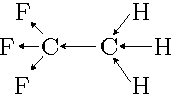
\includegraphics[width=2.5cm]{figs/electronegativity/inductive_effect.pdf}
        \end{figure}
    \end{sol}
\end{problem}

\begin{problem}{}{electronegativity4}
    Используя определение электроотрицательности по Малликену объясните, почему электроотрицательность катиона \ce{Na^+} выше, чем у нейтрального атома натрия?

    \begin{sol}{\ref{prob:electronegativity4}}
        При образовании катиона \ce{Na^+} электрон удаляется с внешней орбитали (ВЗАО). Новая ВЗАО (2p) имеет более низкую энергию, следовательно, потенциал ионизации увеличится. НСАО становится 3s (вместо 3p у нейтрального атома), и из-за уменьшения экранирования сродство к электрону также увеличивается. В соответствии с формулой Малликена оба эти эффекта приводят к увеличению электроотрицательности.
    \end{sol}
\end{problem}

\begin{problem}{}{electronegativity5}
    $\bigstar$ \emph{Профессор Недоумелкин} считает, что элементом с \emph{самой высокой электроотрицательностью} является гелий. Ведь из-за устойчивой заполненной электронной оболочки он имеет самое высокое значение потенциала ионизации и низкое значение сродства к электрону. Однако вы полагаете, что его необходимо исключить из рассмотрения. Как вы аргументируете это?

    \begin{sol}{\ref{prob:electronegativity5}}
        Гелий не образует химических связей в обычных условиях и не существует реальных соединений, на основе которых можно было бы определить их энергию. До 2017 года считали, что гелий вообще не образует никаких соединений. Однако затем под очень высоким давлением были синтезированы соединения гелия (например, \ce{Na2He}). Величину его электроотрицательности можно рассчитать теоретически исходя из его потенциала ионизации (\qty{24,59}{\eV}~--- самая высокая среди всех химических элементов) и других параметров, либо экстраполировав тенденции изменения ЭО в периодической таблице. Однако если не существует реальных связей, то понятие электроотрицательности как способности атома удерживать возле себя электроны связи теряет смысл.
    \end{sol}
\end{problem}

\clearpage

\section{Формы организации вещества}

\hspace*{\parindent}Теперь вы знаете, какими типами \hyperref[sec:introduction_to_chemical_bonding]{химической связи} могут быть соединены атомы в соединении. Однако вещество организовано не только на уровне химических связей между атомами, но и \emph{на более высоком уровне}, когда атомы или молекулы образуют пространственные структуры. Причём чаще всего макрофизические свойства веществ\footnote{Макрофизические свойства вещества~--- это характеристики, которые проявляются на макроуровне, то есть могут быть измерены или наблюдаемы без учёта поведения отдельных атомов и молекул. Они описывают поведение вещества как единого целого.} (температура плавления, плотность, электропроводность и пр.) зависят именно от этого уровня организации.

\subsection*{Агрегатное состояние вещества}

Самое общее разделение, с которого следует начать,~--- это, безусловно, различие в агрегатном состоянии веществ. Из курса физики вы знаете, что вещества могут существовать в четырёх агрегатных состояниях:

\begin{itemize}
    \item газообразное;
    \item жидкое;
    \item твёрдое;
    \item \textit{плазма}\footnote{Плазма представляет собой частично или полностью ионизированное вещество, то есть состоящее из свободно существующих электронов, ионов и нейтральных атомов.}.
\end{itemize}

С плазмой мы почти не сталкиваемся в нашей жизни, а вот о других состояниях давайте вспомним.

Самое главное различие между этими тремя агрегатными состояниями~--- это \emph{баланс} между силами взаимодействия между частицами вещества и их средней кинетической энергией. Именно это является причиной настолько разных свойств газов, жидкостей и твёрдых тел (рис.~\ref{fig:states_of_matter}).

\begin{figure}[htbp]
    \centering
    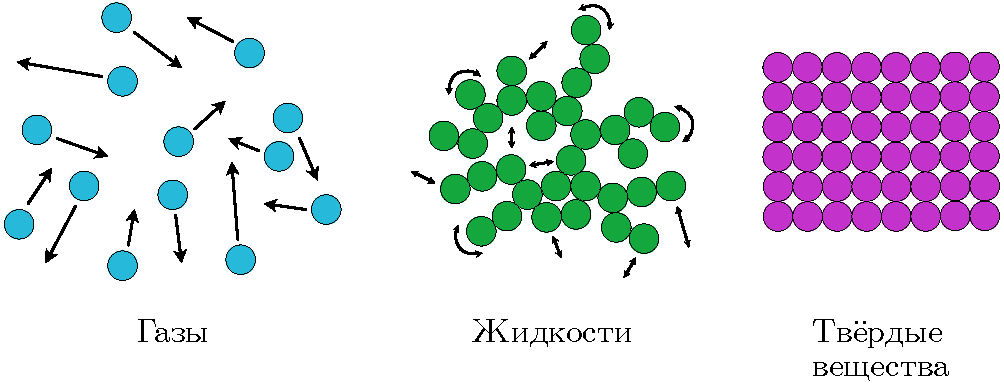
\includegraphics[width=10cm]{figs/forms_of_substance_organization/states_of_matter.pdf}
    \caption{Поведение частиц вещества в газообразном, жидком и твёрдом агрегатных состояниях.}
    \label{fig:states_of_matter}
\end{figure}

Кроме прочных химических связей, соединяющих атомы в веществе, существуют также более слабые, но имеющие большое значение силы взаимодействия между частицами, так называемые \textbf{межмолекулярные силы}\label{term:intermolecular_forces}\index{межмолекулярные силы}. Они всегда являются силами, притягивающими частицы вещества друг к другу, и возникают из-за взаимодействия между зарядами, имеющимися на соседних частицах.

Межмолекулярные силы существуют в любом веществе, даже имеющем устойчивые и незаряженные частицы (именно поэтому существует жидкий гелий), однако они могут иметь очень разную величину, которая зависит, в первую очередь, от \emph{внутреннего строения частиц вещества}.

В то же время частицы обладают некоторой \emph{энергией движения}, зависящей от их температуры, которая стремится разорвать межмолекулярные силы и сделать структуру вещества как можно более неупорядоченной. От того, какие из сил окажутся сильнее, зависит то, в каком агрегатном состоянии будет находиться вещество.

\subsection*{Газообразная форма}

В \emph{газообразной форме} энергия движения частиц значительно выше, чем силы межмолекулярного притяжения, и частицы двигаются с большими скоростями, соударяясь друг с другом и с окружающим веществом, создавая \emph{давление газа}.

Самые характерные свойства газов~--- это их \emph{сжимаемость} и способность \emph{расширяться} до тех пор, пока они не заполнят всё доступное пространство. Поэтому говорят, что у газа нет собственного объёма.

Газы могут неограниченно смешиваться с любыми другими газами, поскольку расстояния между частицами в газе очень велики и они слабо взаимодействуют друг с другом.

При обычных условиях в газообразном состоянии находятся, как правило, соединения или \hyperref[term:chemical_element_substance]{простые вещества} с небольшими молекулами, имеющими ковалентные связи между атомами.

\subsection*{Жидкости}

В \emph{жидкости} межмолекулярные силы и энергия движения частиц сопоставимы по величине. Частицы вещества объединяются друг с другом в плотную среду, сильно ограничивая возможность поступательного движения частиц (оно ограничено <<клеткой>> из соседних частиц). При этом продолжается колебательное и вращательное движение (точнее, вращательные качания) отдельных частей молекул, в результате чего частицы расталкивают друг друга и могут ограниченно перемещаться.

Слои частиц в жидкости могут легко сдвигаться друг относительно друга, приводя к \emph{текучести}.

Вещество в форме жидкости часто имеет \textbf{ближний порядок}\label{term:short-range_order}\index{ближний порядок}. Это означает, что соседние частицы чаще всего повёрнуты друг к другу определённым образом. При этом на дальних расстояниях (например, в нескольких молекулах от рассматриваемой) они могут быть ориентированы с нарушением такой предпочтительности, то есть в жидкостях отсутствует \textbf{дальний порядок}\label{term:long-range_order}\index{дальний порядок}.

\begin{figure}[htbp]
    \centering
    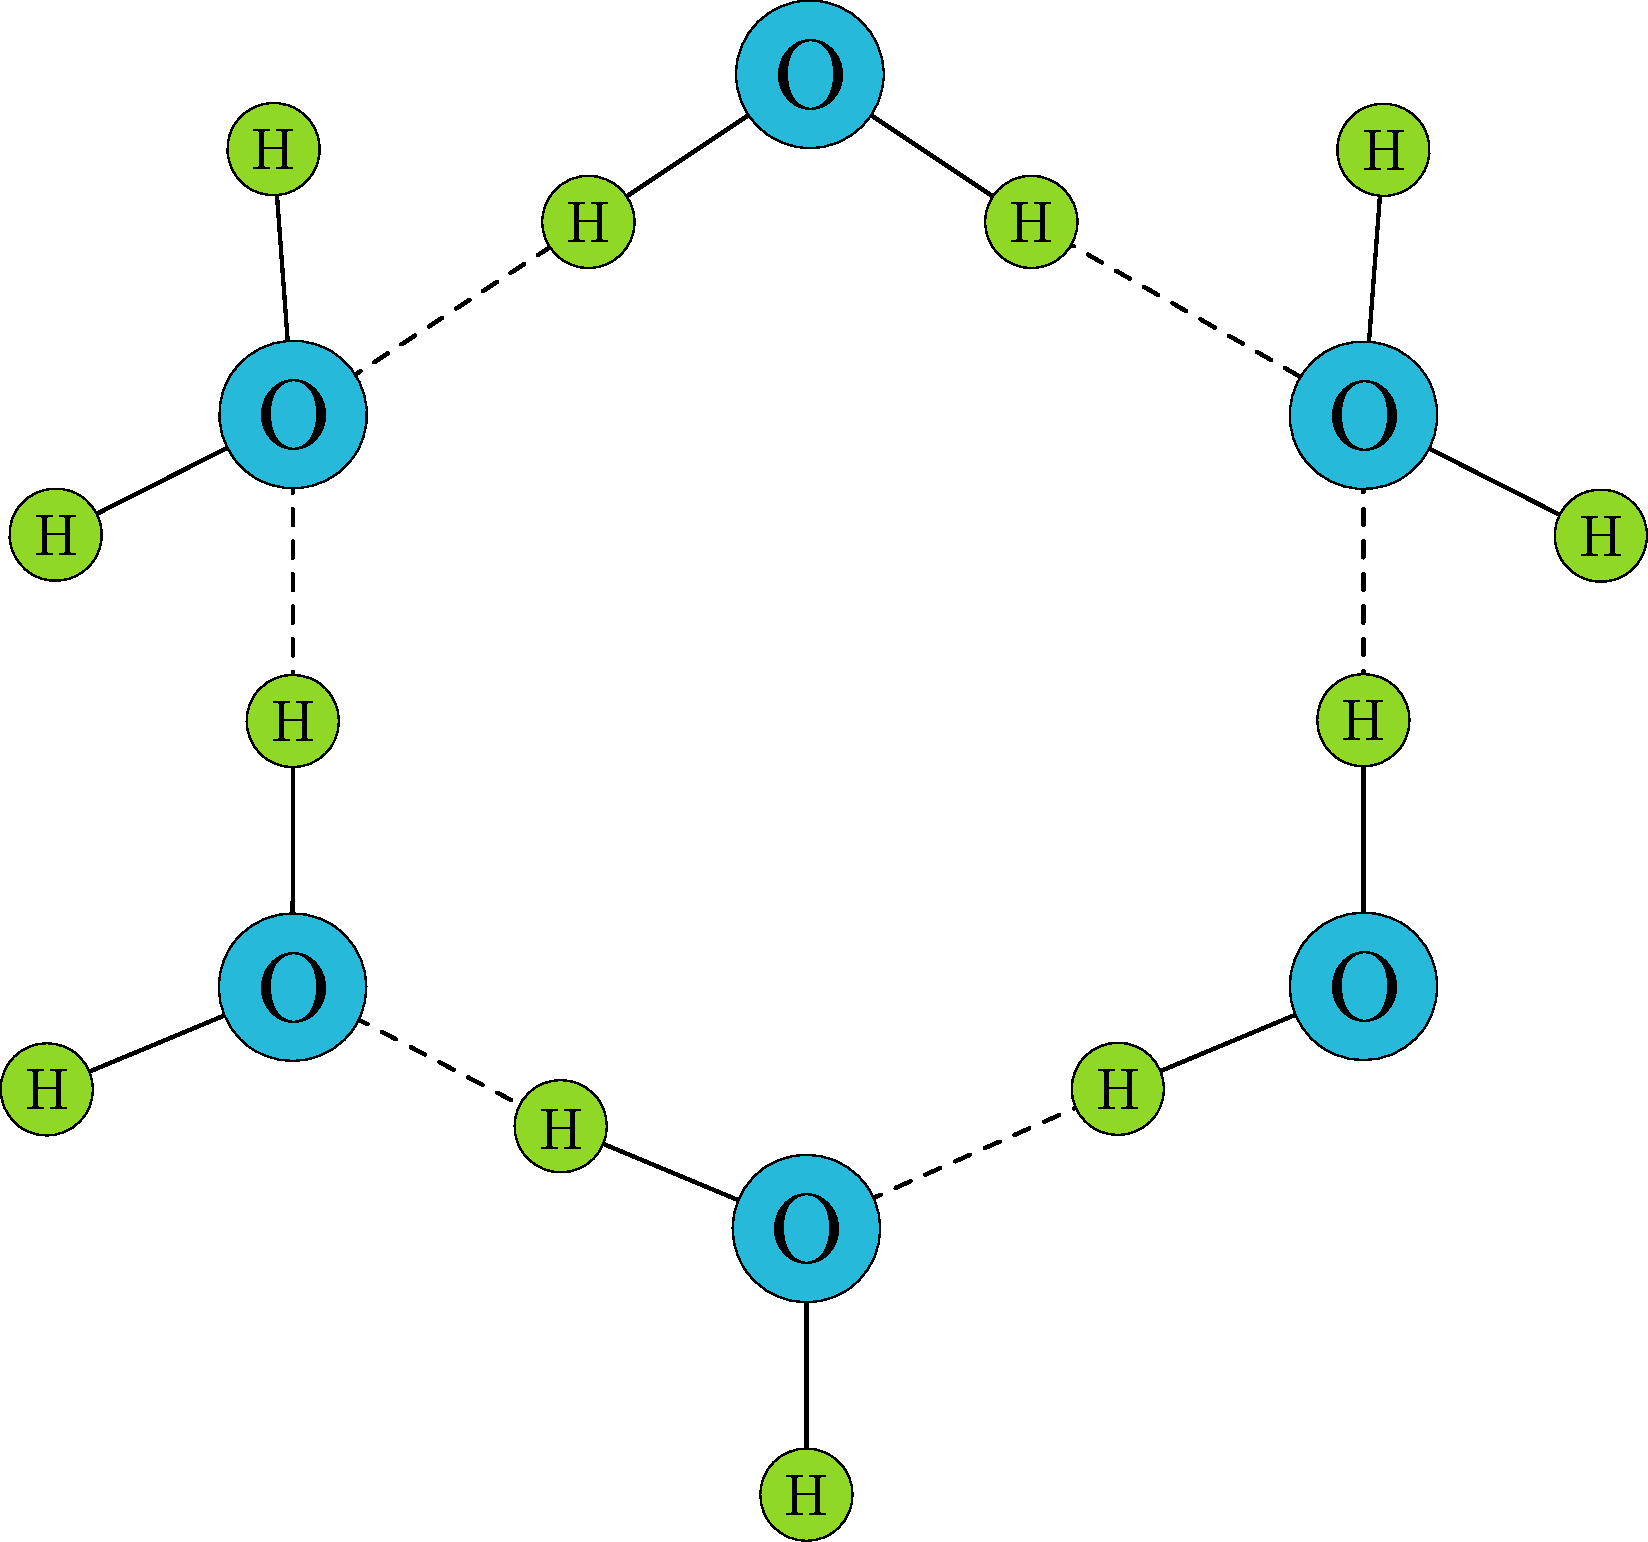
\includegraphics[width=5.5cm]{figs/forms_of_substance_organization/structure_of_liquid_water.pdf}
    \caption{Ближний порядок за счёт водородных связей (показаны пунктирными линиями) в жидкой воде.}
    \label{fig:structure_of_liquid_water}
\end{figure}

Например, в жидкой воде (рис.~\ref{fig:structure_of_liquid_water}) между молекулами образуются довольно прочные межмолекулярные \emph{водородные связи}, которые приводят к структурированию молекул таким образом, что связь \ce{O\bond{1}H} оказывается направленной на атом кислорода соседней молекулы. Однако на больш\'{и}х расстояниях (десятки молекул воды) мы не обнаружим согласования ориентации молекул из-за разупорядочивания вследствие теплового движения.

Жидкости имеют плотность существенно выше, чем газы, более сопоставимую с плотностью твёрдых тел, поэтому жидкость имеет собственный объём. Также жидкости очень трудно сжать: их частицы находятся очень близко друг к другу. В целом можно сказать, жидкости по своему характеру организации значительно ближе к твёрдым телам, чем к газам.

\subsection*{Твёрдые вещества}

В \emph{твёрдых веществах} частицы почти не двигаются и совершают лишь колебательное движение вокруг положений равновесия, а силы межмолекулярного взаимодействия очень значительны. Сжать твёрдые тела очень трудно, частицы в них плотно упакованы.

При этом твёрдые тела имеют довольно много типов внутренней организации. Большинство из этих типов имеют кроме ближнего, также и \emph{дальний} порядок, однако \emph{аморфные} вещества его не имеют.

Давайте подведём итоги рассмотрения свойств веществ в трёх агрегатных состояниях (табл.~\ref{tab:properties_of_states_of_matter}), после чего перейдём к рассмотрению того, каким образом могут быть организованы твёрдые вещества.

\begin{table}[htbp]
    \small
    \caption{Особенности агрегатного состояния вещества.}
    \label{tab:properties_of_states_of_matter}
    \begin{tabularx}{\textwidth}{
        >{\hsize=1\hsize}Y
        >{\hsize=1\hsize}Y
        >{\hsize=1\hsize}Y
        >{\hsize=1\hsize}Y
        }
        \hline
        \rowcolor{green!5}
        Свойство & Газообразное & Жидкое & Твёрдое \\
        \hline
        Кинетическая энергия частиц & Высокая & Средняя & Низкая (колебательное движение) \\
        \hline
        Межмолекулярные силы & Очень слабые & Средние & Сильные \\
        \hline
        Расстояние между частицами & Очень большие & Небольшие & Небольшие \\
        \hline
        Структура & Отсутствует & Ближний порядок & Ближний и дальний или только ближний порядок \\
        \hline
    \end{tabularx}
\end{table}

\subsection*{Строение твёрдых веществ}

Твёрдые вещества по типу организации имеют довольно сложную классификацию. Приведём её на рис.~\ref{fig:forms_of_substance_organization}, дополнив уже имеющуюся классификацию веществ по агрегатному состоянию.

\begin{figure}[htbp]
    \centering
    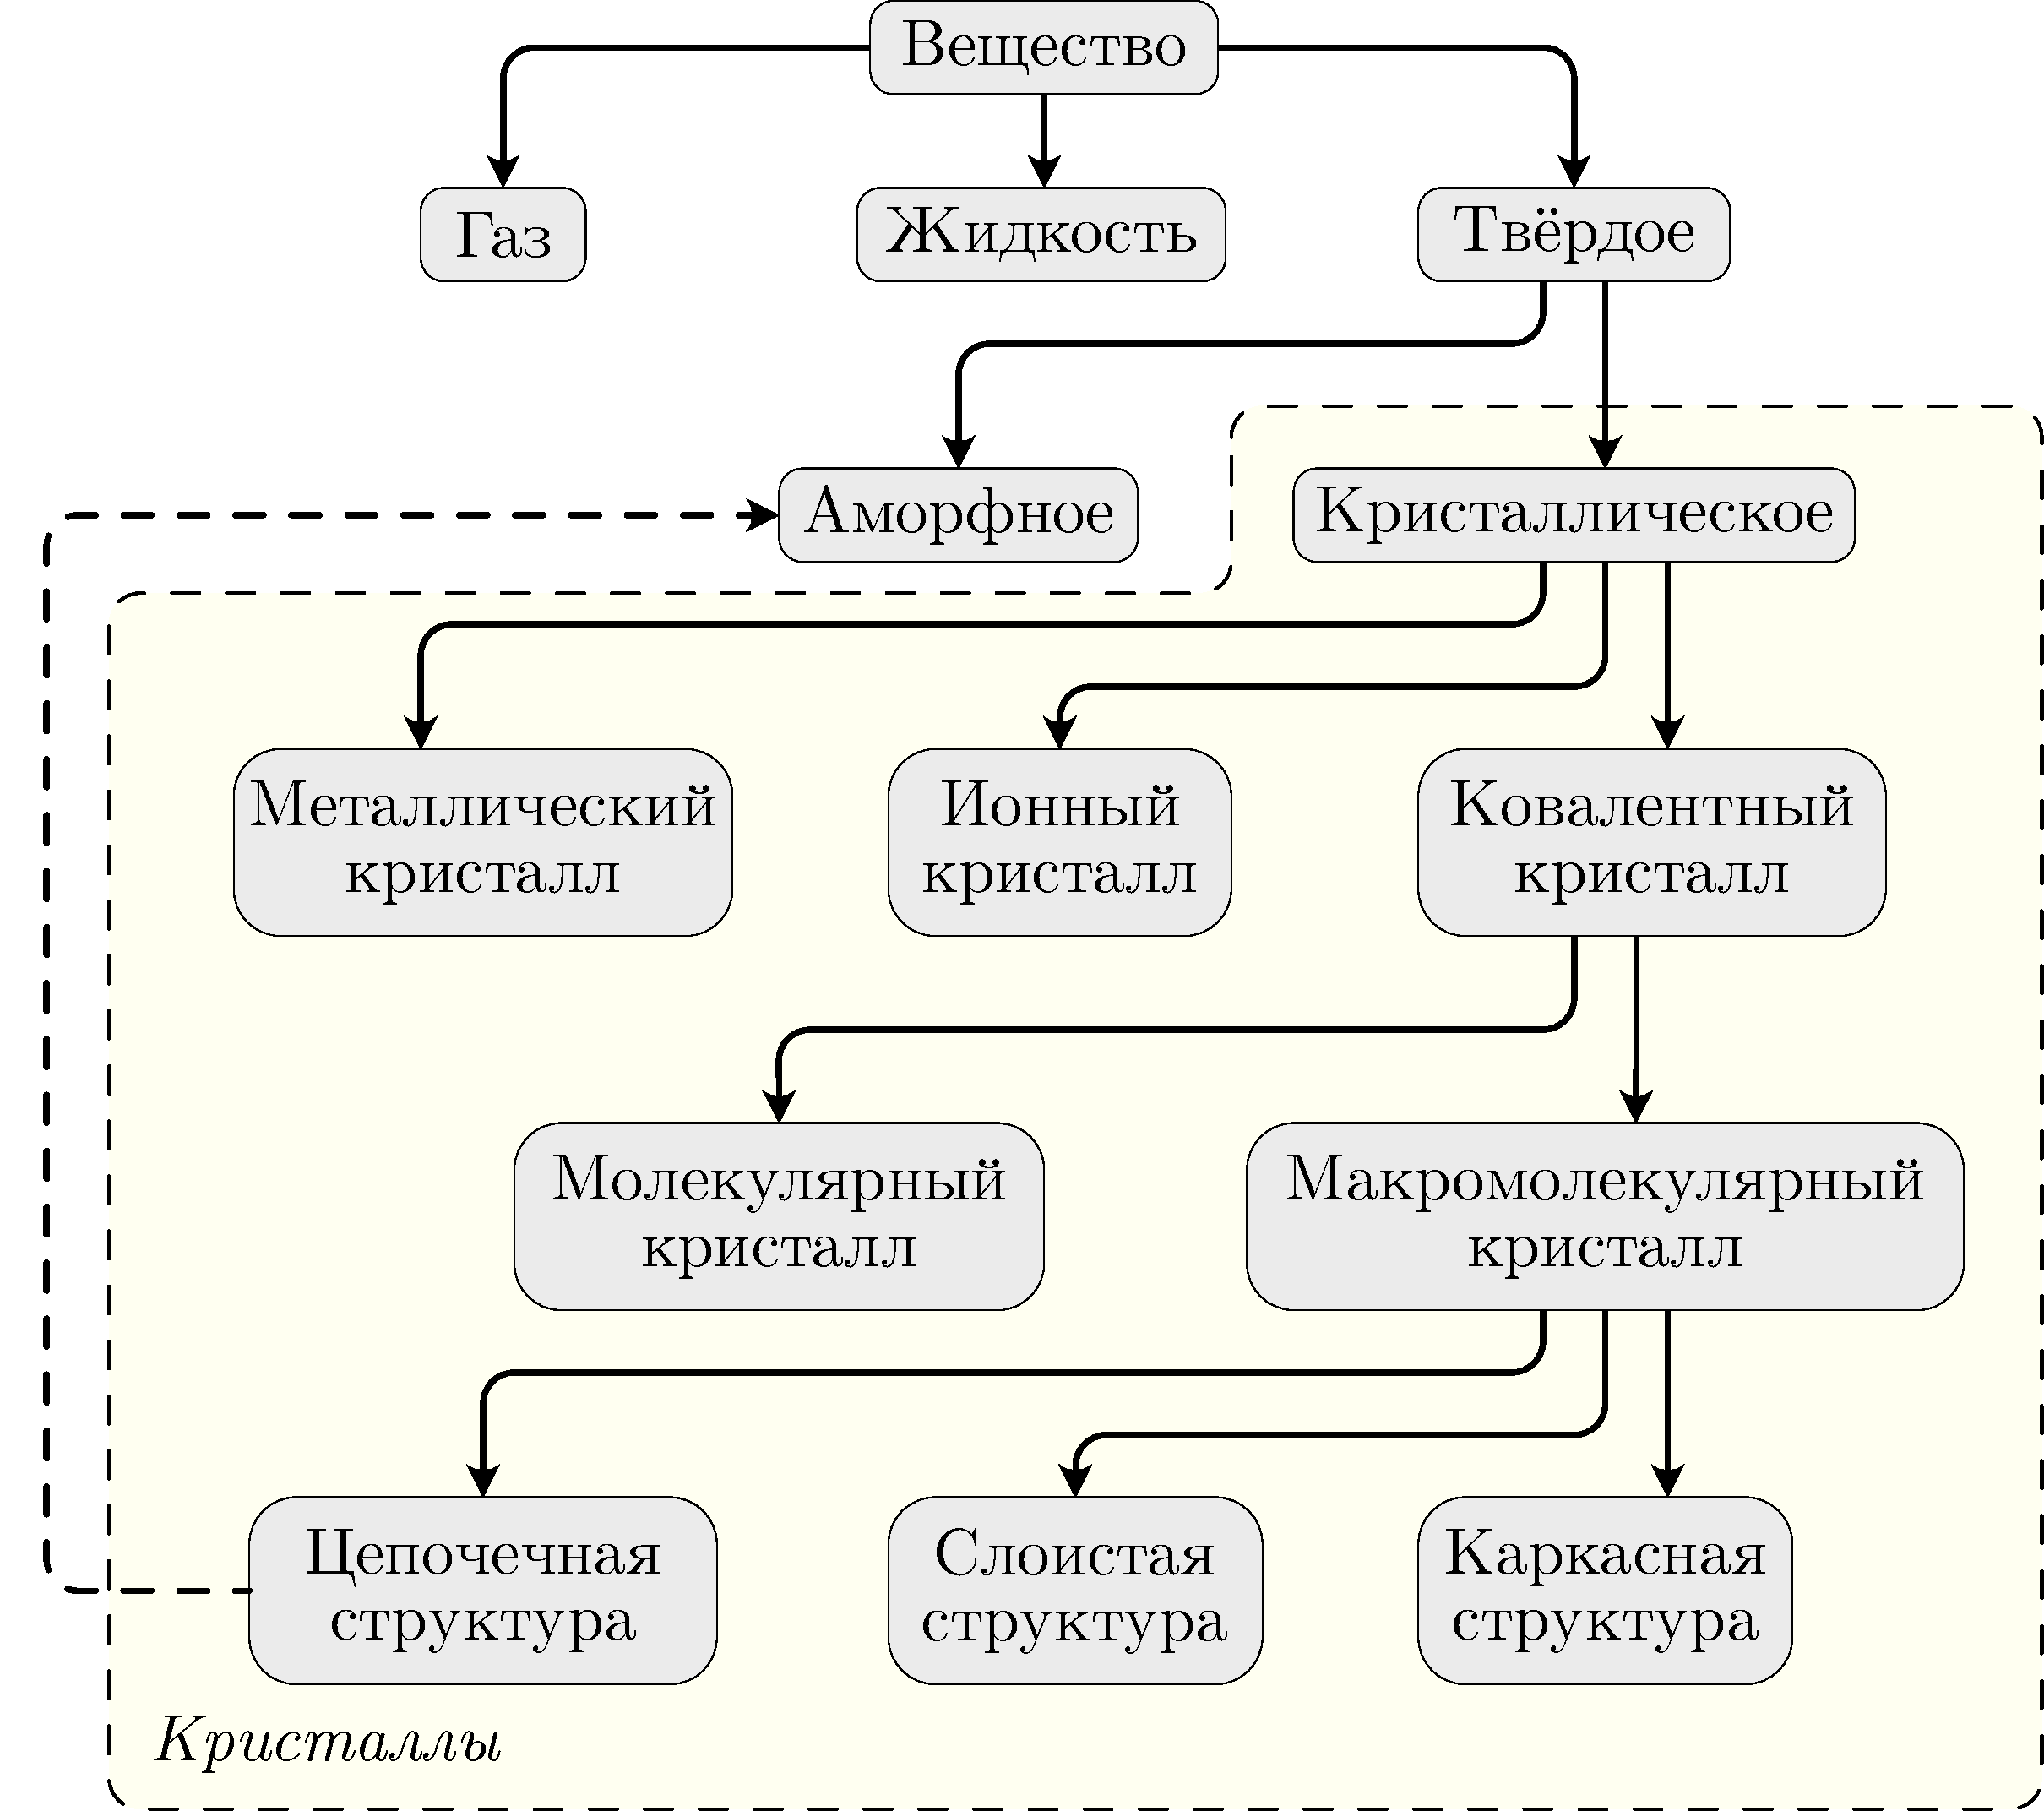
\includegraphics[width=9cm]{figs/forms_of_substance_organization/forms_of_substance_organization.pdf}
    \caption{Формы организации веществ.}
    \label{fig:forms_of_substance_organization}
\end{figure}

В самом общем виде твёрдые вещества делятся на \textbf{кристаллические}\label{term:crystalline_substance}\index{кристаллическое вещество} и \textbf{аморфные}\label{term:amorphous_substance}\index{аморфное вещество}.

Первые представляют собой вещества с наличием дальнего порядка и являются наиболее распространёнными. Примеры кристаллических веществ: хлорид натрия, борная кислота, иод в твёрдом состоянии, водяной лёд.

Аморфные вещества имеют сильные межмолекулярные силы, но имеют только ближний порядок. Типичным примером аморфного вещества является стекло.

Также аморфными являются многие органические вещества с крупными молекулами различной величины, например, полимеры\footnote{Хотя полимеры могут существовать и в кристаллическом состоянии.}. Это связано с тем, что их длинные и часто разветвлённые молекулы сложно уложить в кристаллическую решётку. Органические вещества с небольшими молекулами, как правило, образуют кристаллы, поскольку их компактные молекулы легче упорядочить.

Структура кристаллических веществ представляет собой \textbf{кристаллическую решётку}\label{term:crystal_lattice}\index{кристаллическая решётка}, состоящую из повторяющихся групп частиц, ориентированных определённым образом~--- \textbf{элементарных ячеек}\label{term:unit_cell}\index{элементарная ячейка} (рис.~\ref{fig:crystal_lattice}).

\begin{figure}[htbp]
    \centering
    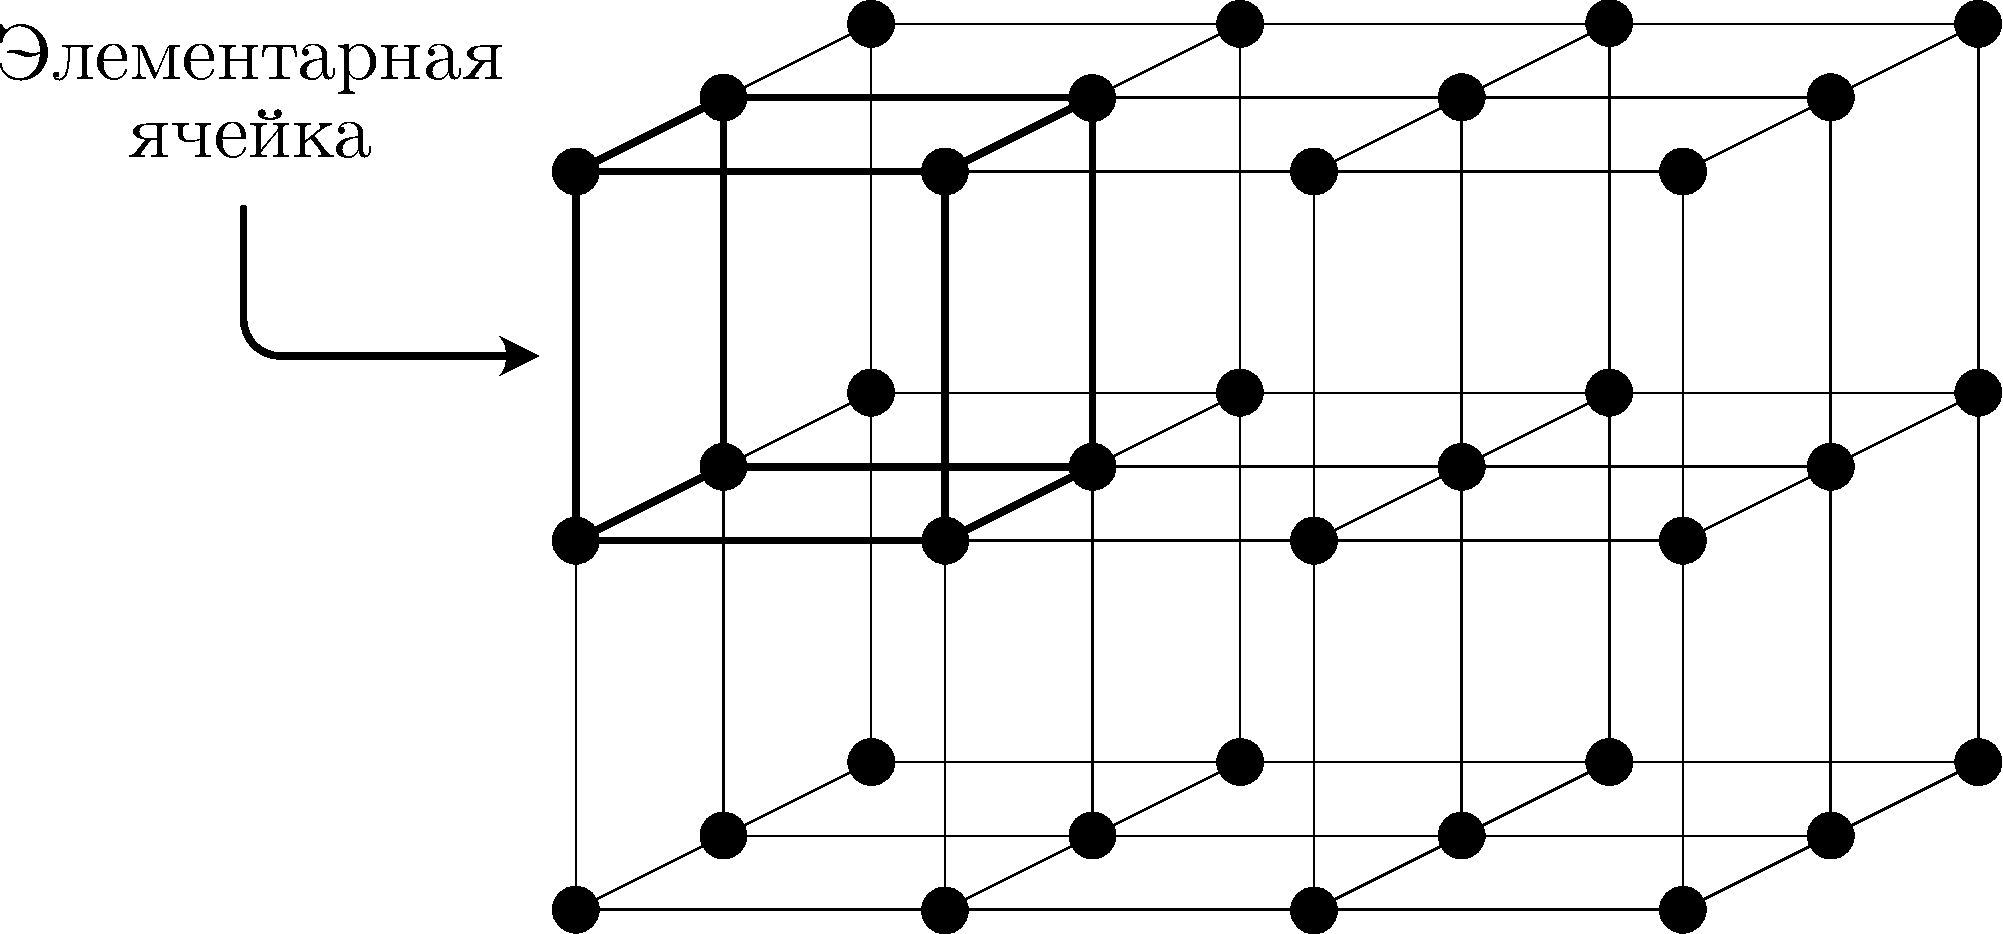
\includegraphics[width=7cm]{figs/forms_of_substance_organization/crystal_lattice.pdf}
    \caption{Пример кристаллической решётки (кубической). Выделена элементарная ячейка.}
    \label{fig:crystal_lattice}
\end{figure}

Элементарные ячейки решёток состоят из \textbf{узлов}\label{term:lattice_points}\index{узлы кристаллической решётки}, отмеченных на рис.~\ref{fig:crystal_lattice} чёрными точками, в которых находятся частицы вещества (атомы, молекулы, ионы). Узлы соединены воображаемыми \textbf{линиями решётки}\label{term:lattice_vectors}\index{линии кристаллической решётки}.

Линии решётки необязательно должны совпадать с направлением связей между частицами, они необходимы лишь для того, чтобы понять структуру элементарной ячейки и отнести её к тому или иному типу.

Элементарные ячейки могут быть многообразны по расположению узлов и линий (рис.~\ref{fig:examples_of_crystal_lattices}). То, к какому типу будет принадлежать решётка, определяется в основном соотношением числа частиц разного типа (например, анионов и катионов) и их размера.

\begin{figure}[htbp]
    \centering
    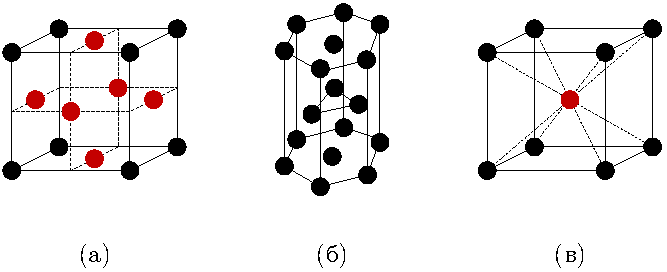
\includegraphics[width=8cm]{figs/forms_of_substance_organization/examples_of_crystal_lattices.pdf}
    \caption{Примеры элементарных ячеек: (а)~--- гранецентрированная кубическая (вложенная); (б)~--- гексагональная плотная упаковка; (в)~--- объёмноцентрированная кубическая (вложенная).}
    \label{fig:examples_of_crystal_lattices}
\end{figure}

Термин <<вложенная>> ячейка означает, что частицы разного типа (например, катионы и анионы), составляющие ячейку, образуют взаимно проникающие друг в друга фигуры.

Например, в \emph{гранецентрированной кубической решётке} (рис.~\ref{fig:examples_of_crystal_lattices} (а)) вершины кубов одного типа частиц совпадают с гранями кубов другого типа частиц. В \emph{объёмноцентрированных ячейках} кубы вложены таким образом, что вершина одной ячейки совпадает с центром другой ячейки (рис.~\ref{fig:body-centered_cubic_lattice}).

\begin{figure}[htbp]
    \centering
    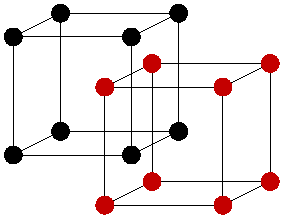
\includegraphics[width=3cm]{figs/forms_of_substance_organization/body-centered_cubic_lattice.pdf}
    \caption{Вложенность ячеек в объёмноцентрированной решётке.}
    \label{fig:body-centered_cubic_lattice}
\end{figure}

Кристаллические вещества имеют чёткую температуру плавления из-за наличия упорядоченной структуры. Когда температура достигает значения температуры плавления, энергия, поступающая к телу, идёт на разрушение кристаллической решётки, а не на дальнейшее повышение температуры. Поэтому плавление происходит при постоянной температуре.

Аморфные вещества плавятся постепенно, размягчаясь в некотором диапазоне температур, потому что в них нет единой структуры, которую нужно разрушать. Частицы расположены хаотично, и при нагревании они постепенно получают достаточно энергии для перехода в жидкое состояние.

\subsection*{Металлический кристалл}

В узлах кристаллических решёток металлов все частицы идентичны, поэтому металлы образуют относительно простые варианты упаковки (по сравнению со сложными ионными и молекулярными). Два основных варианта размещения одинаковых атомов на плоскости~--- \emph{гексагональный} и \emph{квадратный}, которые в совокупности с типом трёхмерной упаковки приводят к трём типам элементарных ячеек (рис.~\ref{fig:types_of_packing_in_metallic_crystals}).

\begin{figure}[htbp]
    \centering
    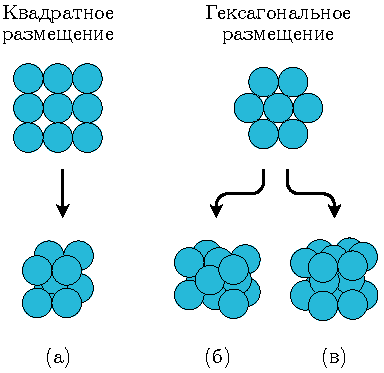
\includegraphics[width=6cm]{figs/forms_of_substance_organization/types_of_packing_in_metallic_crystals.pdf}
    \caption{Типы ячеек в металлах: (а)~--- объёмноцентрированная кубическая; (б)~---гранецентрированная кубическая; (в)~---гексагональная плотная упаковка.}
    \label{fig:types_of_packing_in_metallic_crystals}
\end{figure}

Примеры металлов с различным типом элементарных ячеек приведены в табл.~\ref{tab:types_of_packing_in_metallic_crystals}.

\begin{table}[htbp]
    \small
    \caption{Металлы с различным типом элементарных ячеек.}
    \label{tab:types_of_packing_in_metallic_crystals}
    \begin{tabularx}{\textwidth}{
        >{\hsize=1\hsize}Y
        >{\hsize=1\hsize}Y
        >{\hsize=1\hsize}Y
        }
        \hline
        \rowcolor{green!5}
        Объёмноцентрированная кубическая & Гранецентрированная кубическая & Гексагональная плотная \\
        \hline
        Хром & Алюминий & Магний \\
        Железо & Свинец & Титан \\
        Вольфрам & Медь & Бериллий \\
        Молибден & Платина & Осмий \\
        \hline
    \end{tabularx}
\end{table}

\subsection*{Ионный кристалл}

Ионные кристаллы образуют, например, бромид цезия, оксид магния, гидроксид натрия, нитрат калия.

В ионных кристаллах имеется \hyperref[term:ionic_bond]{ионный тип связи} между находящимися в узлах кристаллической решётки частицами.

В этом случае в узлах располагаются разные по типу частицы: катионы и анионы. Поэтому в ионных кристаллах очень важно разместить ионы в узлах так, чтобы они чередовались по знаку: соседнее расположение ионов одного знака будет приводить к нестабильности. Ионные кристаллы проще рассматривать, мысленно совмещая ячейки катионов и анионов отдельно, как это показано на рис.~\ref{fig:body-centered_cubic_lattice}.

Ионные кристаллы часто имеют объёмноцентрированные и гранецентрированные кубические ячейки (рис.~\ref{fig:examples_of_crystal_lattices}~(а) и~(в)), однако зачастую имеют более сложное строение ячеек, например, триклинное или ромбическое.

\begin{figure}[htbp]
    \centering
    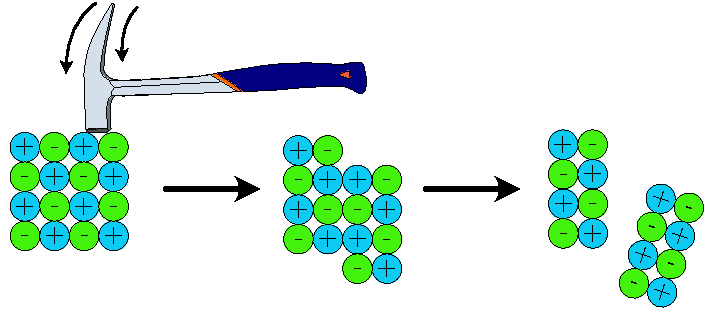
\includegraphics[width=9cm]{figs/forms_of_substance_organization/fragility_of_ionic_crystals.pdf}
    \caption{Причина хрупкости ионных кристаллов.}
    \label{fig:fragility_of_ionic_crystals}
\end{figure}

Ионные связи довольно сильные, поэтому ионные кристаллы тугоплавкие и твёрдые. Однако при этом они хрупкие, так как даже незначительное смещение слоёв кристалла приводит к взаимодействию одноимённых зарядов и раскалыванию (рис.~\ref{fig:fragility_of_ionic_crystals}).

\subsection*{Ковалентный кристалл}

В ковалентном кристалле в том или ином виде имеются \hyperref[term:non-polar_covalent_bond]{ковалентные} связи, а также могут присутствовать межмолекулярные связи. Выделяют два общих типа ковалентных кристалла в зависимости от распределения ковалентных связей.

В первом типе ковалентные связи имеются \emph{только внутри соединений}, находящихся в узлах решётки; в таком случае кристалл называют \textbf{молекулярным}\label{term:molecular_crystal}\index{молекулярный кристалл}. Между отдельными частицами в узлах решётки при этом не ковалентные, а более слабые межмолекулярные связи.

Например, такой тип кристаллической решётки имеет твёрдый \ce{CO2}, который построен в виде кубических гранецентрированных ячеек (рис.~\ref{fig:CO2_crystal_lattice}).

\begin{figure}[htbp]
    \centering
    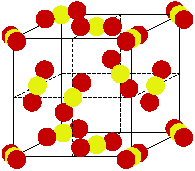
\includegraphics[width=4cm]{figs/forms_of_substance_organization/CO2_crystal_lattice.pdf}
    \caption{Кристаллическая решётка диоксида углерода.}
    \label{fig:CO2_crystal_lattice}
\end{figure}

Молекулярные кристаллы легкоплавки из-за слабых связей между молекулами и очень непрочны механически. Например, молекулярный кристалл воды (лёд) легко колется и плавится при \qty{0}{\degreeCelsius}. Кристаллы иода легко распадаются при умеренном нагревании и превращаются в пар.

Если ковалентные связи в кристалле имеются и \emph{между узлами решётки}, образуя пространственную матрицу, то такой кристалл называют \textbf{макромолекулярным}\label{term:macromolecular_crystal}\index{макромолекулярный кристалл}. В таких кристаллах в узлах решётки могут располагаться только отдельные атомы. В зависимости от структуры выделяют три типа таких кристаллов: \textbf{цепочечные}\label{term:chain-structured_crystal}\index{цепочечный кристалл}, \textbf{слоистые}\label{term:layered_crystal}\index{слоистый кристалл} и \textbf{каркасные}\label{term:framework_crystal}\index{каркасный кристалл}.

\subsection*{Цепочечный кристалл}

Классический пример подобного соединения~---соединения металлов с хлором, имеющие ковалентные полярные связи, например, хлорид бериллия \ce{BeCl2}.

Такие соединения образуют протяжённые цепочечные структуры, образованные при помощи донорно-акцепторных связей\footnote{Если быть точнее, то это мостиковые ковалентные связи с частичным донорно-акцепторным характером.} между соседними молекулами \ce{BeCl2} (рис.~\ref{fig:chain-structured_crystal}).

\begin{figure}[htbp]
    \centering
    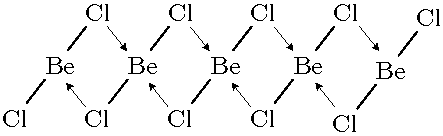
\includegraphics[width=6cm]{figs/forms_of_substance_organization/chain-structured_crystal.pdf}
    \caption{Цепочечная структура хлорида бериллия \ce{BeCl2}.}
    \label{fig:chain-structured_crystal}
\end{figure}

Длина таких цепочек может варьироваться, и часто подобные соединения по своим свойствам могут напоминать аморфные соединения. Поэтому на рис.~\ref{fig:forms_of_substance_organization} от цепочечного кристалла имеется дополнительная пунктирная стрелка к аморфным веществам. Иногда такое строение имеют и простые вещества, например, селен и теллур.

\subsection*{Слоистый кристалл}

Такие кристаллы состоят из прочных слоёв, в которых атомы связаны ковалентными связями. Слои при этом соединены между собой слабыми межмолекулярными связями.

Примером вещества такого типа является графит (одна из форм углерода). В нём гексагональные ячейки, лежащие в одной плоскости, образуют слой, который слабо связан с такими же соседними слоями (рис.~\ref{fig:graphite_structure}).

\begin{figure}[htbp]
    \centering
    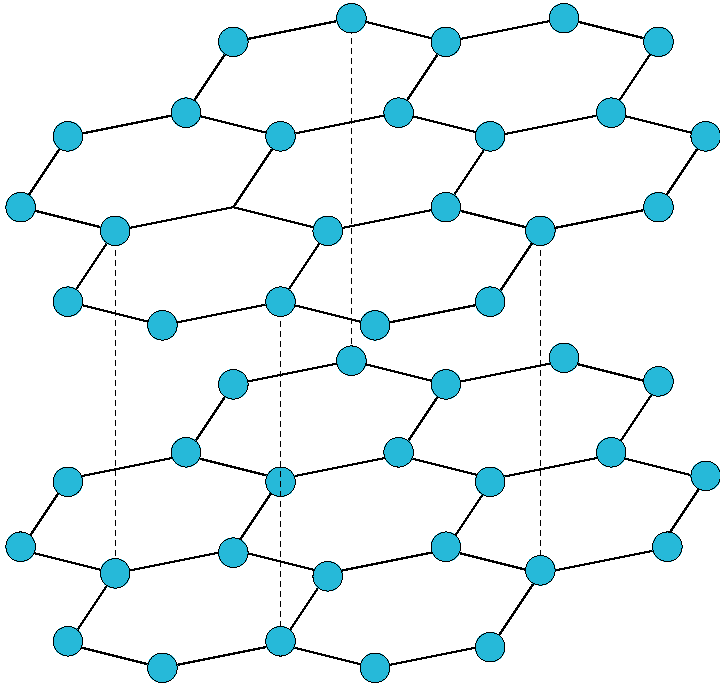
\includegraphics[width=4.5cm]{figs/forms_of_substance_organization/graphite_structure.pdf}
    \caption{Слоистая структура графита.}
    \label{fig:graphite_structure}
\end{figure}

Такое строение приводит к тому, что слои в таком кристалле легко отделяются друг от друга, поэтому такие материалы легко расслаиваются, а также являются сравнительно мягкими и непрочными.

Например, графит используют в грифелях карандашей, где он расслаивается при соприкосновании с бумагой, оставляя на ней след. Графит также обладает способностью проводить электрический ток, поэтому его также используют в качестве электродов в промышленности. 

\subsection*{Каркасный кристалл}

Каркасные кристаллы образуют трёхмерную матрицу ковалентных связей, по существу представляя собой гигантскую макромолекулу.

Самый известный пример каркасного кристалла~--- это алмаз (ещё одна форма углерода). В нём каждый атом соединяется с четырьмя такими же атомами углерода (рис.~\ref{fig:diamond_lattice}), образуя тетраэдры, которые повторяются до бесконечности (точнее, до границы кристалла).

\begin{figure}[htbp]
    \centering
    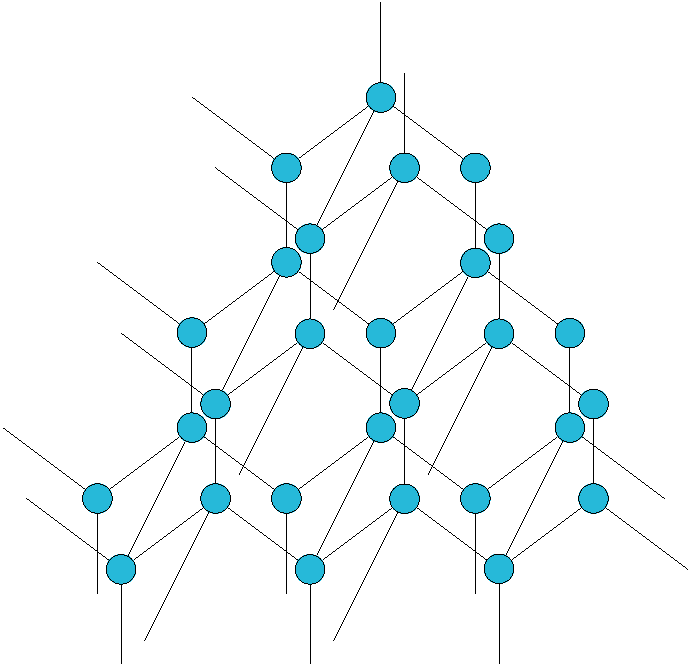
\includegraphics[width=4.5cm]{figs/forms_of_substance_organization/diamond_lattice.pdf}
    \caption{Каркасная структура алмаза.}
    \label{fig:diamond_lattice}
\end{figure}

Следствием такого строения является очень \emph{высокая твёрдость} каркасных кристаллов, поскольку нагрузки на него могут равномерно распределяться по сетке ковалентных связей.

Кроме того, поскольку все связи в каркасных кристаллах очень прочные, такой кристалл очень трудно расплавить.

Тот же алмаз плавится при температурах порядка \num{3700}--\qty{4000}{\degreeCelsius} и давлениях порядка \qty{110000}{\atm}.

\subsection*{Свойства кристаллов и их строение}

Подведём итоги того, как строение кристаллических веществ влияет на их физические свойства. Соберём всю информацию в табл.~\ref{tab:properties_of_crystal_lattices}.

Чаще всего, даже основываясь на подобных довольно простых признаках, можно сделать вывод о типе организации того или иного вещества.

\begin{table}[htbp]
    \small
    \caption{Влияние типа кристаллической решётки на свойства вещества.}
    \label{tab:properties_of_crystal_lattices}
    \begin{tabularx}{\textwidth}{
        >{\hsize=1\hsize}Y
        >{\hsize=1\hsize}Y
        >{\hsize=1\hsize}Y
        >{\hsize=1\hsize}Y
        >{\hsize=1\hsize}Y
        }
        \hline
        \rowcolor{green!5}
        Свойство & Металлический кристалл & Ионный\newline кристалл & Молекулярный кристалл & Макромолекулярный \\
        \hline
        Что в узлах решётки & Атомы\newline металла & Ионы & Молекулы & Атомы \\
        \hline
        Тип связи между узлами & Металлический & Ионный & Межмолекулярный & Ковалентный или межмолекулярный \\
        \hline
        Температуры плавления и кипения & Высокие & Высокие & Низкие & Различные \\
        \hline
        Механические свойства & Твёрдые,\newline тягучие & Твёрдые, хрупкие & Мягкие, непрочные & Различные \\
        \hline
        Электропроводность & Отличная & Диэлектрик & Диэлектрик & Чаще всего диэлектрики (исключение~--- графит) \\
        \hline
    \end{tabularx}
\end{table}

\begin{termlist}
    \hyperref[term:intermolecular_forces]{Межмолекулярные силы}, 
    \hyperref[term:short-range_order]{ближний порядок},
    \hyperref[term:long-range_order]{дальний порядок},
    \hyperref[term:crystalline_substance]{кристаллическое вещество},
    \hyperref[term:amorphous_substance]{аморфное вещество},
    \hyperref[term:crystal_lattice]{кристаллическая решетка},
    \hyperref[term:unit_cell]{элементарная ячейка},
    \hyperref[term:lattice_points]{узлы кристаллической решётки},
    \hyperref[term:lattice_vectors]{линии кристаллической решётки},
    \hyperref[term:molecular_crystal]{молекулярный кристалл},
    \hyperref[term:macromolecular_crystal]{макромолекулярный кристалл},
    \hyperref[term:chain-structured_crystal]{цепочечный кристалл},
    \hyperref[term:layered_crystal]{слоистый кристалл},
    \hyperref[term:framework_crystal]{каркасный кристалл}.
\end{termlist}

\begin{problem}{}{forms_of_substance_organization1}
    Основываясь на ваших знаниях о типичных свойствах, присущих тому или иному типу организации твёрдых веществ, постарайтесь догадаться, к какому типу относятся следующие вещества.
    \begin{enumerate}[label=\arabic*)]
        \item Поваренная соль;
        \item Латунь;
        \item Битум;
        \item Замёрзший спирт;
        \item Смола;
        \item Кварц;
        \item Тальк.
    \end{enumerate}
    \begin{sol}{\ref{prob:forms_of_substance_organization1}}
        \begin{enumerate}[label=\arabic*)]
            \item Ионный кристалл;
            \item Металлический кристалл;
            \item Аморфное вещество;
            \item Молекулярный кристалл;
            \item Аморфное вещество;
            \item Каркасный кристалл;
            \item Слоистый кристалл.
    \end{enumerate}
    \end{sol}
\end{problem}

\clearpage

\section{Валентность и степень окисления}

\hspace*{\parindent}Состояние атома в соединении химики оценивают с двух точек зрения:

\begin{itemize}
    \item числа образуемых связей (валентности);
    \item электронного состояния атома (степени окисления).
\end{itemize}

Целесообразно рассмотреть оба подхода сразу, чтобы избежать путаницы между ними.

\subsection*{Валентность}

Атомы химических элементов могут образовывать разное количество связей с другими атомами в зависимости от состояния их электронной оболочки и того, с какими атомами они образуют связь.

При этом существуют элементы (например, щелочные и щелочноземельные металлы)\footnote{\emph{Щелочными} называют все элементы подгруппы Ia, а \emph{щелочноземельными}~--- IIa. Существует несколько общепринятых традиционных классов химических элементов. Их классификация показана в \hyperref[appendix:periodic_table]{периодической таблице} при помощи различных цветов заливки ячеек.}, которые всегда образуют одно и то же количество связей (например, всегда одну или две), но существуют и элементы, которые могут формировать \emph{переменное} количество связей (азот, хлор, медь и др.).

Количество связей, которые образует атом, называется \textbf{валентностью}\label{term:valence}\index{валентность} атома. Валентность элементов обозначают арабскими цифрами.

Приведём примеры валентностей, которые проявляют химические элементы, в табл.~\ref{tab:valence_of_chemical_elements}, разделив элементы с постоянной и переменной валентностью.

\begin{table}[htbp]
    \small
    \caption{Валентности химических элементов.}
    \label{tab:valence_of_chemical_elements}
    \begin{tabularx}{\textwidth}{
        >{\hsize=1.7\hsize}Y
        >{\hsize=0.5\hsize}Z
        >{\hsize=0.8\hsize}Z
        }
        \hline
        \rowcolor{green!5}
        Элементы & Валентность & Примеры \\
        \hline
        \rowcolor{yellow!5}
        \ce{Li}, \ce{Na}, \ce{K}, \ce{F}, \ce{H} & 1 & \ce{Na2O}, \ce{HF} \\
        \hline
        \rowcolor{yellow!5}
        \ce{Be}, \ce{Mg}, \ce{Ca}, \ce{Zn}, \ce{O} & 2 & \ce{MgCl2}, \ce{ZnO} \\
        \hline
        \rowcolor{yellow!5}
        \ce{B}, \ce{Al}, \ce{Ga}, \ce{Sc}, \ce{La} & 3 & \ce{Al(OH)3}, \ce{H3BO3} \\
        \hline
        \rowcolor{blue!5}
        \ce{Cu} & 1 и 2 & \ce{CuO}, \ce{Cu2O} \\
        \hline
        \rowcolor{blue!5}
        \ce{Co}, \ce{Fe} & 2 и 3 & \ce{CoCl3}, \ce{Fe2O3} \\
        \hline
        \rowcolor{blue!5}
        \ce{C}, \ce{Si}, \ce{Sn}, \ce{Pb} & 2 и 4 & \ce{CO}, \ce{SiO2} \\
        \hline
        \rowcolor{blue!5}
        \ce{S} & 2, 4 и 6 & \ce{H2S}, \ce{SO2}, \ce{H2SO4} \\
        \hline
    \end{tabularx}
\end{table}

\subsection*{Степень окисления}

Степень окисления была введена в химии по двум причинам:

\begin{itemize}
    \item чтобы классифицировать вещества на окислители и восстановители;
    \item для упрощения расстановки коэффициентов в уравнениях окислительно-восстановительных реакций.
\end{itemize}

Чтобы понять, какой же смысл несёт эта величина, вначале объясним такую понятие, как \textbf{ионное приближение}\label{term:ionic_approximation}\index{ионное приближение}. Это допущение, которое предполагает, что любое химическое соединение состоит только из ионов.

Рассмотрим молекулу хлороводорода, состоящую из двух атомов~--- водорода и хлора, которые имеют по одному неспаренному электрону и образуют между собой связь. Какому из атомов принадлежит пара электронов, образующая связь? На самом деле ни водороду, ни хлору, потому что электронная плотность связи концентрируется между обоими атомами, и никому не принадлежит, хотя смещается к атому, у которого выше электроотрицательность, в данном случае к хлору.

В такой ситуации ионное приближение говорит, что пара электронов связи считается принадлежащей тому атому, у которого больше электроотрицательность, то есть хлору (рис.~\ref{fig:shift_of_the_electron_pair_in_HCl}).

\begin{figure}[htbp]
    \centering
    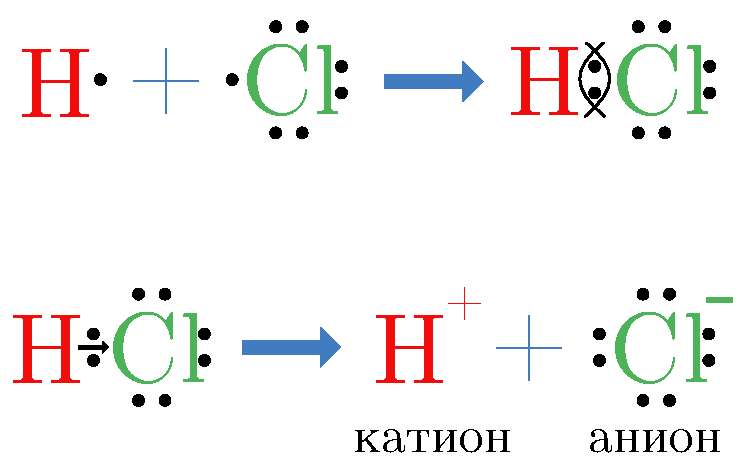
\includegraphics[width=3.5cm]{figs/valence_and_oxidation_state/shift_of_the_electron_pair_in_HCl.pdf}
    \caption{Перемещение электронных пар связи в ионном приближении.}
    \label{fig:shift_of_the_electron_pair_in_HCl}
\end{figure}

Поскольку считается, что хлор полностью забрал электронную пару связи, то он превращается в отрицательно заряженный ион~--- \emph{анион}. Атом, у которого забрали электроны связи, наоборот, превращается в \emph{катион}~--- положительно заряженный ион. Если подобную процедуру перемещения электронных пар провести со всеми связями в молекуле, то мы получим все атомы соединения в виде ионов, а заряды этих ионов и будут степенями окисления.

Таким образом, \textbf{степень окисления}\label{term:oxidation_state}\index{степень окисления}~--- это условный заряд атома в соединении, вычисленный исходя из предположения, что молекула состоит только из ионов.

Разумеется, атомы в соединениях чаще всего не являются ионами, но степень окисления~--- это \emph{формальное допущение}, потому что с ней удобно работать на практике.

Степень окисления элемента \emph{в формуле соединения} обозначается арабскими цифрами с указанием знака (плюса в том числе) над элементом, например:

\begin{equation*}
    \overset{+1}{\ce{H}}_2\overset{-2}{\ce{O}},\;\overset{+5}{\ce{P}}_2\overset{-2}{\ce{O}}_5,\;\overset{+1}{\ce{H}}\overset{+1}{\ce{Cl}}\overset{-2}{\ce{O}}.
\end{equation*}

Обратите внимание, что знак степени окисления, плюс или минус, ставится \emph{перед} числом. Если же записывается заряд иона, то знак ставится уже \emph{после} числа. Например, для сульфат-аниона запись с указанием степеней окисления и общего заряда иона будет выглядеть так:

\begin{equation*}
    (\overset{+6}{\ce{S}}\overset{-2}{\ce{O4}})^{2-}.
\end{equation*}

В \emph{названии соединения} степень окисления указывается в круглых скобках в конце названия. При этом указывают только степень окисления того элемента, который \emph{проявляет переменную степень окисления}, например: хлорид меди (I), оксид железа (II). Если элемент проявляет постоянную степень окисления, то её не указывают.

Максимальную положительную степень окисления, которую может проявлять химический элемент, определяется количеством электронов на внешнем электронном уровне и равна \emph{номеру группы} периодической таблицы, в которой находится элемент. Например, хлор находится в седьмой группе и может проявлять максимальную степень окисления +7.

Однако данное правило не выполняется для элементов с высокой электроотрицательностью и для некоторых благородных газов. Хотя эти элементы формально находятся в группах с большими номерами, они не могут проявлять в соединениях теоретическую максимальную степень окисления. Это элементы: \emph{кислород}, \emph{фтор}, а также \emph{гелий}, \emph{неон} и \emph{аргон}.

\subsection*{Как рассчитывается степень окисления}

Для расчёта степени окисления используются следующие правила.

Обычно химические элементы проявляют некоторые типичные для себя степени окисления. Например, у кислорода в соединениях чаще всего степень окисления равна $-2$ (\ce{CO2}, \ce{H2SO4}), а у водорода~--- чаще всего $+1$ (\ce{PH3}, \ce{CH4}). Иногда элементы могут проявлять и другие, менее распространённые для себя степени окисления. Например, во фториде кислорода \ce{OF2} степень окисления кислорода равна $+2$. В гидриде натрия \ce{NaH} степень окисления водорода равна $-1$. 

Возможные степени окисления элементов вы можете найти в \hyperref[appendix:periodic_table]{периодической таблице} в конце учебника. Наиболее типичные степени выделены полужирным шрифтом.

Считается, что элементы с большей электроотрицательностью в соединениях проявляют более низкую степень окисления относительно элементов с меньшей электроотрицательностью. Например, в воде $\overset{+1}{\ce{H2}}\overset{-2}{\ce{O}}$ степень окисления водорода положительна, а у кислорода отрицательна, потому что у кислорода больше электроотрицательность, а вот во фториде кислорода $\overset{+2}{\ce{O}}\overset{-1}{\ce{F2}}$ наоборот, потому что электроотрицательность фтора больше, чем у кислорода.

Для многих элементов характерна только одна степень окисления (как и валентность), другие они проявлять просто не могут в силу особенностей электронного строения атома. Например, все щелочные металлы (\ce{Li}, \ce{Na}, \ce{K} и др.) проявляют в соединениях только степень окисления $+1$, щелочноземельные (\ce{Ca}, \ce{Mg}, \ce{Ba} и др.) всегда имеют степень окисления $+2$. Фтор в соединениях всегда имеет степень окисления $-1$.

Простые вещества, т.~е. состоящее из одинаковых атомов (\ce{H2}, \ce{O2}, \ce{P4}) имеют степень окисления, равную нулю, поскольку невозможно <<присвоить>> электроны связи ни одному из атомов.

Степень окисления одноатомных ионов вроде \ce{S^{2-}} или \ce{Cl^-} равна заряду этого иона. Например, для сульфид-иона степень окисления серы равна $-2$: $\overset{-2}{\ce{S^{2-}}}$. Это правило является следствием баланса по зарядам, о котором сейчас пойдёт речь.

Правило \textbf{баланса по зарядам}\label{term:charge_balance}\index{баланс по зарядам} заключается в следующем: если сложить все степени окисления всех атомов в молекуле, то получится величина заряда молекулы. Например, для воды $\overset{+1}{\ce{H2}}\overset{-2}{\ce{O}}$ можно записать такой баланс: два атома водорода со степенью окисления $+1$, плюс один атом кислорода со степенью окисления $-2$. В сумме это равно нулю, поэтому молекула воды в целом не заряжена:

\begin{equation*}
    2 \cdot (+1) + 1 \cdot (-2) = 0.
\end{equation*}

Для фосфат-аниона $(\overset{+5}{\ce{P}}\overset{-2}{\ce{O4}})^{3-}$ баланс по зарядам приводит к заряду $-3$, что соответствует общему заряду этого аниона:

\begin{equation*}
    1 \cdot (+5) + 4 \cdot (-2) = -3.
\end{equation*}

Степень окисления для отдельно взятого атома не может быть дробной, однако, \emph{средняя} степень окисления для всех атомов одного химического элемента в молекуле может. Например, для кислорода:

\begin{itemize}
    \item в воде она равна $-2$ (типичная степень окисления),
    \item в пероксиде водорода \ce{H2O2} равна $-1$ (пониженная степень окисления),
    \item в супероксиде натрия \ce{NaO2} равна $-\frac{1}{2}$,
    \item в озониде натрия \ce{NaO3} она вообще равна $-\frac{1}{3}$.
\end{itemize}

Такие формальные степени окисления являются следствием двух причин:

\begin{itemize}
    \item в составе вещества находятся атомы одного химического элемента в разных степенях окисления (например, в оксиде железа (II, III) \ce{Fe3O4} имеются атомы железа со степенями окисления $+2$ и $+3$);
    \item атомы в соединении эквивалентны, но заряд распределён между ними (супероксид и озонид натрия).
\end{itemize}

Обратите внимание, что степень окисления не равна валентности. Например, валентность углерода в органических соединениях, как правило, равна четырём (потому что он образует четыре связи с соседними атомами), однако степень окисления у него может быть различной:

\begin{itemize}
    \item $-4$ (в метане \ce{CH4}),
    \item $-2$ (в метаноле \ce{CH3OH}),
    \item $0$ (в формальдегиде \ce{CH2O}),
    \item $+2$ (в муравьиной кислоте \ce{HCOOH}).
\end{itemize}

\subsection*{Расчёт степени окисления по брутто-формуле вещества}

\textbf{Брутто-формулой}\label{term:molecular_formula}\index{брутто-формула} называют формулу, отражающую состав целой молекулы. Существует также \textbf{эмпирическая формула}\label{term:empirical_formula}\index{эмпирическая формула}, которая отражает только соотношение атомов. Например, брутто-формула уксусной кислоты~--- \ce{C2H4O2}, а её эмпирическая формула~--- \ce{CH2O}.

Порядок расчёта степеней окисления по этому методу следующий:

\begin{enumerate}[label=\arabic*)]
    \item Для элементов, проявляющих типичные степени окисления, или способных проявлять только одну степень окисления (водород, кислород, щелочные и щёлочноземельные металлы) сразу записываем их степени окисления.
    \item Затем для элементов, степень окисления которых неизвестна, обозначаем её переменной и составляем баланс по зарядам. Из него находим неизвестные степени окисления.
    \item Если соединение сложное по структуре (например, содержит несколько атомов, которые проявляют разные степени окисления), стараемся разбить его на более простые фрагменты, а затем уже вычисляем степень окисления отдельно в каждом фрагменте.
\end{enumerate}

Рассмотрим этот метод на примере оксида железа \ce{Fe2O3}. У кислорода в соединениях степень окисления обычно равна $-2$. Пусть $x$~--- это степень окисления железа в этом соединении:

\begin{equation*}
    \overset{x}{\ce{Fe2}}\overset{-2}{\ce{O3}}.
\end{equation*}

Заряд молекулы в целом равен нулю. Отсюда записываем баланс по зарядам:

\begin{equation*}
    2 \cdot x + 3 \cdot (-2) = 0,
\end{equation*}
\begin{equation*}
    x = +3.
\end{equation*}

\subsection*{Расчёт степени окисления по структурной формуле вещества}

Часто бывает, что атомы одного химического элемента в соединении проявляют разные степени окисления, поскольку находятся в разных местах молекулы или образуют разное количество связей. В этом случае удобно использовать данный метод расчёта. Чтобы определить степень окисления атома, рисуют структуру молекулы и для каждого атома рассматривают образуемые им связи. Если элемент, с которым имеется связь, более электроотрицателен, чем рассматриваемый атом, то связь <<отдают>> этому элементу. Если связь образуют два одинаковых элемента, то связь не отдают никому и не учитывают. Итоговая степень окисления атома равна:

\begin{equation*}
    \text{СО} = N_{\text{отд}} - N_{\text{пол}},
\end{equation*}

где $N_{\text{отд}}$ и $N_{\text{пол}}$~--- число отданных и полученных атомом связей. В качестве примера приведём расстановку степеней окисления в пероксоазотистой кислоте \ce{HNO3}, в которой есть неэквивалентные атомы кислорода (рис.~\ref{fig:peroxonitrous_acid}).

\begin{figure}[htbp]
    \centering
    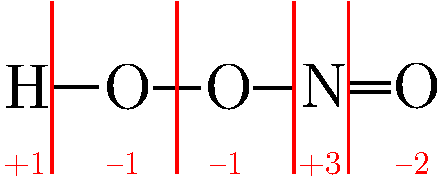
\includegraphics[width=2.8cm]{figs/valence_and_oxidation_state/peroxonitrous_acid.pdf}
    \caption{Пероксоазотистая кислота.}
    \label{fig:peroxonitrous_acid}
\end{figure}

Атом водорода образует всего одну связь с атомом кислорода, который более электроотрицателен, поэтому связь <<отдаём>> кислороду, а степень окисления водорода равна:

\begin{equation*}
    \text{СО}_\text{H} = 1 - 0 = +1.
\end{equation*}

Следующий атом кислорода помимо уже описанной связи имеет связь с другим атомом кислорода, которую мы не учитываем, потому что она образована двумя одинаковыми атомами, поэтому:

\begin{equation*}
    \text{СО}_\text{O} = 0 - 1 = -1.
\end{equation*}

Повторяя процедуру для всех атомов, находим все оставшиеся степени окисления.

Рассмотрим ещё один интересный пример~--- уксусную кислоту \ce{CH3COOH}.

Для начала запишем формулу уксусной кислоты в виде брутто-формулы~--- \ce{C2H4O2}, а затем, учитывая, что степень окисления водорода $+1$, а кислорода $-2$, найдём степень окисления углерода:

\begin{equation*}
    \overset{x}{\ce{C2}}\overset{+1}{\ce{H4}}\overset{-2}{\ce{O2}},
\end{equation*}
\begin{equation*}
    2 \cdot x + 4 \cdot (+1) + 2 \cdot (-2) = 0,
\end{equation*}
\begin{equation*}
    x = 0,
\end{equation*}
\begin{equation*}
    \overset{0}{\ce{C2}}\overset{+1}{\ce{H4}}\overset{-2}{\ce{O2}}.
\end{equation*}

Однако здесь есть один нюанс. Если записать формулу уксусной кислоты в виде структурной формулы, то становится понятно, что атомы углерода в ней неэквивалентны и имеют разные значения степени окисления:

\begin{figure}[htbp]
    \centering
    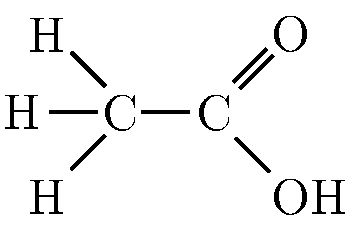
\includegraphics[width=2.5cm]{figs/valence_and_oxidation_state/acetic_acid_without_oxidation_states.pdf}
\end{figure}

Однако расчёт степени окисления по брутто-формуле дал нам степень окисления ноль, потому что такой расчёт даёт \emph{усреднённую} степень окисления и для сложных молекул приводит к неверным результатам. Для нахождения правильных степеней окисления воспользуемся методом перемещения связей:

\begin{figure}[htbp]
    \centering
    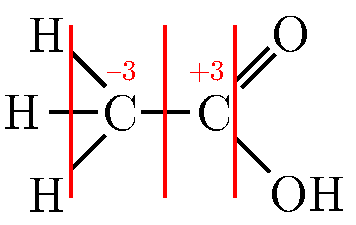
\includegraphics[width=2.5cm]{figs/valence_and_oxidation_state/acetic_acid_with_oxidation_states.pdf}
\end{figure}

\begin{example}{}{ex:valence_and_oxidation_state1}
    \textit{Расставьте степени окисления в перманганате калия \ce{KMnO4}.}

    \medskip

    \textit{Решение.} Кислород и калий проявляют типичные степени окисления: у калия степень окисления всегда $+1$, а у кислорода обычно $-2$. Степень окисления марганца обозначим за $x$:
    \begin{equation*}
        \overset{+1}{\ce{K}}\overset{x}{\ce{Mn}}\overset{-2}{\ce{O4}}.
    \end{equation*}
    Составляем баланс по зарядам, учитывая, что молекула не заряжена:
    \begin{equation*}
        1 \cdot (+1) + 1 \cdot x + 4 \cdot (-2) = 0,
    \end{equation*}
    \begin{equation*}
        x = +7.
    \end{equation*}
    Следовательно, степень окисления марганца в перманганате калия равна +7:
    \begin{equation*}
        \overset{+1}{\ce{K}}\overset{+7}{\ce{Mn}}\overset{-2}{\ce{O4}}.
    \end{equation*}
\end{example}

\begin{example}{}{ex:valence_and_oxidation_state2}
    \textit{Рассмотрим случай, когда кислород проявляет нетипичную для себя степень окисления~--- в молекуле пероксида водорода \ce{H2O2}.}

    \medskip

    \textit{Решение.} Водород способен проявлять три степени окисления: $-1$ в гидридах, 0 в молекулярном водороде и $+1$ во всех остальных случаях. Поскольку электроотрицательность кислорода гораздо выше, чем у водорода, то очевидно, что он будет отнимать у него электроны и водород будет проявлять степень окисления $+1$. Степень окисления кислорода обозначим $x$, общий заряд молекулы равен нулю. Составляем баланс по зарядам:
    \begin{equation*}
        \overset{+1}{\ce{H2}}\overset{x}{\ce{O2}},
    \end{equation*}
    \begin{equation*}
        2 \cdot (+1) + 2 \cdot x = 0,
    \end{equation*}
    \begin{equation*}
        x = -1.
    \end{equation*}
    Таким образом, степень окисления кислорода в этом соединении равна $-1$.
\end{example}

\begin{example}{}{ex:valence_and_oxidation_state3}
    \textit{Рассмотрим ещё одно соединение, в котором кислород проявляет нетипичную степень окисления~--- фторид кислорода \ce{O2F2}.}

    \medskip

    \textit{Решение.} Кислород в целом очень электроотрицательный элемент, как правило, именно он окисляет атомы других химических элементов. Однако фтор самый электроотрицательный элемент и может только принимать электроны. Степень окисления у него в соединениях всегда одна и та же: $-1$. Принимаем степень окисления кислорода за $x$ и составляем баланс по зарядам:
    \begin{equation*}
        \overset{x}{\ce{O2}}\overset{-1}{\ce{F2}},
    \end{equation*}
    \begin{equation*}
        2 \cdot x + 2 \cdot (-1) = 0,
    \end{equation*}
    \begin{equation*}
        x = +1.
    \end{equation*}
    То есть в этом соединении кислород находится в степени окисления $+1$.
\end{example}

\begin{example}{}{ex:valence_and_oxidation_state4}
    \textit{Следующий пример~--- моноклинная сера. Она находится в состоянии молекул с формулой \ce{S8}.}

    \medskip

    \textit{Решение.} В данном случае можно сразу написать степень окисления ноль, потому что это простое вещество.
    \begin{equation*}
        \overset{0}{\ce{S8}}.
    \end{equation*}
    Как уже было сказано выше, нулевую степень окисления при образовании связи между одинаковыми атомами можно объяснить так: поскольку оба атома, образующие связь, обладают одинаковой электроотрицательностью, электроны связи не смещены ни к одному из атомов, т.~е. образуется ковалентная неполярная связь. Другими словами, ни один из атомов даже формально не может принять на себя электроны связи.
\end{example}

\begin{example}{}{ex:valence_and_oxidation_state5}
    \textit{Теперь рассмотрим расчёт степеней окисления в заряженных частицах, например, в карбонат-анионе \ce{CO3^{2-}}.}

    \medskip

    \textit{Решение.} В этом случае расчёт проводится по обычной схеме, за исключением того, что сумма всех степеней окисления атомов равна заряду молекулы.
    \begin{equation*}
        (\overset{x}{\ce{C}}\overset{-2}{\ce{O3}})^{2-},
    \end{equation*}
    Для кислорода записываем типичную степень окисления $-2$, и, учитывая, что карбонат-анион имеет в целом заряд $-2$, записываем баланс по зарядам:
    \begin{equation*}
        1 \cdot x + 3 \cdot (-2) = -2,
    \end{equation*}
    \begin{equation*}
        x = +4.
    \end{equation*}
\end{example}

\begin{example}{}{ex:valence_and_oxidation_state6}
    \textit{Теперь давайте посмотрим ещё один интересный пример~--- оксид железа \ce{Fe3O4}.}

    \medskip

    \textit{Решение.} Степень окисления кислорода равна $-2$, тогда степень окисления железа в соединении после составления баланса и расчёта получается равной
    \begin{equation*}
        3 \cdot x + 4 \cdot (-2) = 0,
    \end{equation*}
    \begin{equation*}
        x = +\frac{8}{3}.
    \end{equation*}
    В этом соединении \emph{формальная} степень окисления железа равна $+\frac{8}{3}$. Однако электроны не перемещаются частями, а только по одному. Дело в том, что данное соединение на самом деле представляет собой смесь оксидов железа (II) и (III):
    \begin{equation*}
       \overset{+2}{\ce{Fe}}\overset{-2}{\ce{O}} \cdot \overset{+3}{\ce{Fe}}\overset{-2}{\ce{O}}.
    \end{equation*}
    Всегда помните, что расчёт степени окисления по брутто-формуле вещества хорошо работает только для простых несложных молекул.
\end{example}

\begin{example}{}{ex:valence_and_oxidation_state7}
    \textit{Разберём ещё один пример расстановки степеней окисления~--- нитрат аммония \ce{NH4NO3}.}

    \medskip

    \textit{Решение.} В нитрате аммония имеется два атома азота, которые могут проявлять разные степени окисления, поэтому, когда мы будем записывать баланс по зарядам, у нас получится уравнение с двумя неизвестными, поэтому разделим это соединение на две устойчивые частицы~--- катион аммония \ce{NH4^+} и нитрат-анион \ce{NO3^-}, и в каждой из них отдельно посчитаем степень окисления азота. Для катиона аммония:
    \begin{equation*}
        1 \cdot x + 4 \cdot (+1) = +1,
    \end{equation*}
    \begin{equation*}
        x = -3.
    \end{equation*}
    Для нитрат-аниона:
    \begin{equation*}
        1 \cdot x + 3 \cdot (-2) = -1,
    \end{equation*}
    \begin{equation*}
        x = +5.
    \end{equation*}
    Записываем степени окисления для всей молекулы и делаем проверку. Для этого составляем баланс по зарядам с рассчитанными степенями окисления и проверяем, сходится ли он:
    \begin{equation*}
        \overset{-3}{\ce{N}}\overset{+1}{\ce{H4}}\overset{+5}{\ce{N}}\overset{-2}{\ce{O3}},
    \end{equation*}
    \begin{equation*}
        (-3) + 4 \cdot (+1) + 1 \cdot (+5) + 3 \cdot (-2) = 0.
    \end{equation*}
    Баланс сходится, значит, степени окисления были определены верно.
\end{example}

\subsubsection*{Различие между валентностью и степенью окисления}

Давайте подведём итоги и сопоставим два изученных в этом разделе понятия. Покажем ключевые моменты в табл.~\ref{tab:difference_between_valence_and_oxidation_state}.

\begin{table}[htbp]
    \small
    \caption{Различия между валентностью и степенью окисления.}
    \label{tab:difference_between_valence_and_oxidation_state}
    \begin{tabularx}{\textwidth}{
        >{\hsize=0.8\hsize}Y
        >{\hsize=1.1\hsize}Y
        >{\hsize=1.1\hsize}Y
        }
        \hline
        \rowcolor{green!5}
        Характеристика & Валентность & Степень окисления \\
        \hline
        Физический смысл & Число связей, образуемых атомом & Условный заряд атома в соединении \\
        \hline
        Значения & Всегда положительное число (или 0) & Положительная, отрицательная или нулевая \\
        \hline
        Чем определяется & Структурой связей & Электроотрицательностью элементов \\
        \hline
        Значения & Целые числа & Целые и дробные числа \\
        \hline
    \end{tabularx}
\end{table}

В качестве примера того, что валентность не равна нулю даже в случае нулевой степени окисления, можно взять любое простое вещество, например, азот. В молекуле азота \ce{N2} атомы связаны между собой тройной связью, поэтому валентность каждого из атомов равна трём. Однако электроны связи не смещены ни к одному из атомов, поэтому степень окисления азота в молекуле \ce{N2} равна нулю.

\begin{termlist}
    \hyperref[term:valence]{Валентность}, 
    \hyperref[term:ionic_approximation]{ионное приближение},
    \hyperref[term:oxidation_state]{степень окисления},
    \hyperref[term:charge_balance]{баланс по зарядам},
    \hyperref[term:molecular_formula]{брутто-формула},
    \hyperref[term:empirical_formula]{эмпирическая формула}.
\end{termlist}

\begin{problem}{}{valence_and_oxidation_state1}
    Расставьте степени окисления в следующих соединениях: а) \ce{H2O}; б) \ce{O2}; в) \ce{Fe2O3}; г) \ce{FeCl3}; д) \ce{Na2O}; е) \ce{FeO}; ж) \ce{H2S}; з) \ce{HF}.
    \begin{sol}{\ref{prob:valence_and_oxidation_state1}}
        а) $\overset{+1}{\ce{H2}}\overset{-2}{\ce{O}}$; б) $\overset{0}{\ce{O2}}$; в) $\overset{+3}{\ce{Fe2}}\overset{-2}{\ce{O3}}$; г) $\overset{+3}{\ce{Fe}}\overset{-1}{\ce{Cl3}}$; д) $\overset{+1}{\ce{Na2}}\overset{-2}{\ce{O}}$; е) $\overset{+2}{\ce{Fe}}\overset{-2}{\ce{O}}$; ж) $\overset{+1}{\ce{H2}}\overset{-2}{\ce{S}}$; з) $\overset{+1}{\ce{H}}\overset{-1}{\ce{F}}$.
    \end{sol}
\end{problem}

\begin{problem}{}{valence_and_oxidation_state2}
    Расставьте степени окисления в следующих соединениях: а) \ce{Cl2}; б) \ce{K2O}; в) \ce{CaCl2}; г) \ce{HI}; д) \ce{Mg2N3}; е) \ce{CaC2}; ж) \ce{ZnF2}; з) \ce{CO2}.
    \begin{sol}{\ref{prob:valence_and_oxidation_state2}}
        а) $\overset{0}{\ce{Cl2}}$; б) $\overset{+1}{\ce{K2}}\overset{-2}{\ce{O}}$; в) $\overset{+2}{\ce{Ca}}\overset{-1}{\ce{Cl2}}$; г) $\overset{+1}{\ce{H}}\overset{-1}{\ce{I}}$; д) $\overset{+2}{\ce{Mg2}}\overset{-3}{\ce{N3}}$; е) $\overset{+2}{\ce{Ca}}\overset{-1}{\ce{C2}}$; ж) $\overset{+2}{\ce{Zn}}\overset{-1}{\ce{F2}}$; з) $\overset{+4}{\ce{C}}\overset{-2}{\ce{O2}}$.
    \end{sol}
\end{problem}

\begin{problem}{}{valence_and_oxidation_state3}
    Расставьте степени окисления в следующих соединениях: а) \ce{NO2}; б) \ce{ClO2}; в) \ce{N2O}; г) \ce{SO2}; д) \ce{AlCl3}; е) \ce{N2O5}; ж) \ce{PH3}; з) \ce{SiO2}.
    \begin{sol}{\ref{prob:valence_and_oxidation_state3}}
        а) $\overset{+4}{\ce{N}}\overset{-2}{\ce{O2}}$; б) $\overset{+4}{\ce{Cl}}\overset{-2}{\ce{O2}}$; в) $\overset{+1}{\ce{N2}}\overset{-2}{\ce{O}}$; г) $\overset{+4}{\ce{S}}\overset{-2}{\ce{O2}}$; д) $\overset{+3}{\ce{Al}}\overset{-1}{\ce{Cl3}}$; е) $\overset{+5}{\ce{N2}}\overset{-2}{\ce{O5}}$; ж) $\overset{-3}{\ce{P}}\overset{+1}{\ce{H3}}$; з) $\overset{+4}{\ce{Si}}\overset{-2}{\ce{O2}}$.
    \end{sol}
\end{problem}

\begin{problem}{}{valence_and_oxidation_state4}
    Расставьте степени окисления в следующих соединениях: а) \ce{HNO3}; б) \ce{K3PO4}; в) \ce{K2Se}; г) \ce{HMnO4}; д) \ce{TiO2}; е) \ce{H2SO4}; ж) \ce{HBrO}; з) \ce{PbS}; и) \ce{Mn2O7}; к) \ce{NaOH}.
    \begin{sol}{\ref{prob:valence_and_oxidation_state4}}
        а) $\overset{+1}{\ce{H}}\overset{+5}{\ce{N}}\overset{-2}{\ce{O3}}$; б) $\overset{+1}{\ce{K3}}\overset{+5}{\ce{P}}\overset{-2}{\ce{O4}}$; в) $\overset{+1}{\ce{K2}}\overset{-2}{\ce{Se}}$; г) $\overset{+1}{\ce{H}}\overset{+7}{\ce{Mn}}\overset{-2}{\ce{O4}}$; д) $\overset{+4}{\ce{Ti}}\overset{-2}{\ce{O2}}$; е) $\overset{+1}{\ce{H2}}\overset{+6}{\ce{S}}\overset{-2}{\ce{O4}}$; ж) $\overset{+1}{\ce{H}}\overset{+1}{\ce{Br}}\overset{-2}{\ce{O}}$; з) $\overset{+2}{\ce{Pb}}\overset{-2}{\ce{S}}$; и) $\overset{+7}{\ce{Mn2}}\overset{-2}{\ce{O7}}$; к) $\overset{+1}{\ce{Na}}(\overset{-2}{\ce{O}}\overset{+1}{\ce{H}})$.
    \end{sol}
\end{problem}

\begin{problem}{}{valence_and_oxidation_state5}
    Расставьте степени окисления в следующих соединениях: а) \ce{CaSO4}; б) \ce{MgSO4}; в) \ce{Al2(SO4)3}; г) \ce{Mg2P2O7}; д) \ce{HClO3}; е) \ce{SOCl2}; ж) \ce{SO2Cl2}; з) \ce{HNO2}; и) \ce{K2Cr2O7}; к) \ce{NaHCO3}.
    \begin{sol}{\ref{prob:valence_and_oxidation_state5}}
        а) $\overset{+2}{\ce{Ca}}\overset{+6}{\ce{S}}\overset{-2}{\ce{O4}}$; б) $\overset{+2}{\ce{Mg}}\overset{+6}{\ce{S}}\overset{-2}{\ce{O4}}$; в) $\overset{+3}{\ce{Al2}}\left(\overset{+6}{\ce{S}}\overset{-2}{\ce{O4}}\right)_3$; г) $\overset{+2}{\ce{Mg2}}\overset{+5}{\ce{P2}}\overset{-2}{\ce{O7}}$; д) $\overset{+1}{\ce{H}}\overset{+5}{\ce{Cl}}\overset{-2}{\ce{O3}}$; е) $\overset{+4}{\ce{S}}\overset{-2}{\ce{O}}\overset{-1}{\ce{Cl2}}$; ж) $\overset{+6}{\ce{S}}\overset{-2}{\ce{O2}}\overset{-1}{\ce{Cl2}}$; з) $\overset{+1}{\ce{H}}\overset{+3}{\ce{N}}\overset{-2}{\ce{O2}}$; и) $\overset{+1}{\ce{K2}}\overset{+6}{\ce{Cr2}}\overset{-2}{\ce{O7}}$; к) $\overset{+1}{\ce{Na}}\overset{+1}{\ce{H}}\overset{+4}{\ce{C}}\overset{-2}{\ce{O3}}$.
    \end {sol}
 \end {problem}

\begin{problem}{}{valence_and_oxidation_state6}
    Расставьте степени окисления в следующих соединениях: а) \ce{Al(OH)2Cl}; б) \ce{NaH2PO4}; в) \ce{HClO4}; г) \ce{K2S2O7}; д) \ce{Al4C3}; е) \ce{As2O3}; ж) \ce{OF2}; з) \ce{SiH4}; и) \ce{F2O}; к) \ce{Na2FeO4}.
    \begin{sol}{\ref{prob:valence_and_oxidation_state6}}
        а) $\overset{+3}{\ce{Al}}(\overset{-2}{\ce{O}}\overset{+1}{\ce{H}})_2\overset{-1}{\ce{Cl}}$; б) $\overset{+1}{\ce{Na}}\overset{+1}{\ce{H2}}\overset{+5}{\ce{P}}\overset{-2}{\ce{O4}}$; в) $\overset{+1}{\ce{H}}\overset{+7}{\ce{Cl}}\overset{-2}{\ce{O4}}$; г) $\overset{+1}{\ce{K2}}\overset{+6}{\ce{S2}}\overset{-2}{\ce{O7}}$; д) $\overset{+3}{\ce{Al4}}\overset{-4}{\ce{C3}}$; е) $\overset{+3}{\ce{As2}}\overset{-2}{\ce{O3}}$; ж) $\overset{+2}{\ce{O}}\overset{-1}{\ce{F2}}$; з) $\overset{-4}{\ce{Si}}\overset{+1}{\ce{H4}}$; и) $\overset{+2}{\ce{O}}\overset{-1}{\ce{F2}}$; к) $\overset{+1}{\ce{Na2}}\overset{+6}{\ce{Fe}}\overset{-2}{\ce{O4}}$.
    \end{sol}
\end{problem}

\begin{problem}{}{valence_and_oxidation_state7}
    Самые высокие известные степени окисления зафиксированы в катионе тетраоксоиридия \ce{IrO4^+} и катионе тетраоксоплатины \ce{PtO4^(2+)}. Чему они равны?
    \begin{sol}{\ref{prob:valence_and_oxidation_state7}}
        $+9$ и $+10$.
    \end{sol}
\end{problem}

\begin{problem}{}{valence_and_oxidation_state8}
    $\bigstar$ Рассчитайте с использованием структурной формулы степень окисления всех атомов в молекуле хлористого сульфурила \ce{SO2Cl2}.
    \begin{sol}{\ref{prob:valence_and_oxidation_state8}}
        \begin{figure}[htbp]
            \centering
            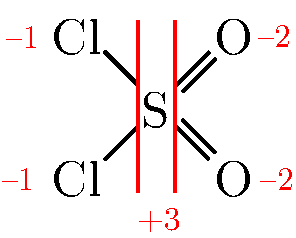
\includegraphics[width=2.5cm]{figs/valence_and_oxidation_state/sulfuryl_chloride.pdf}
        \end{figure}
    \end{sol}
\end{problem}

\begin{problem}{}{valence_and_oxidation_state9}
    $\bigstar$ Рассчитайте с использованием структурной формулы степень окисления всех атомов в молекуле фосфористой кислоты \ce{H3PO3}.
    \begin{sol}{\ref{prob:valence_and_oxidation_state9}}
        Фосфористая кислота, хотя формально и является трёхосновной, обладает только двумя атомами водорода, которые могут отрываться в виде катионов. Причина этого в том, что третий атом водорода образует связь непосредственно с атомом фосфора. При этом ключевым моментом является то, что электроотрицательность водорода немного, но всё-таки выше, чем у атома фосфора, поэтому связь между ними считаем принадлежащей атому водорода.
        \begin{figure}[htbp]
            \centering
            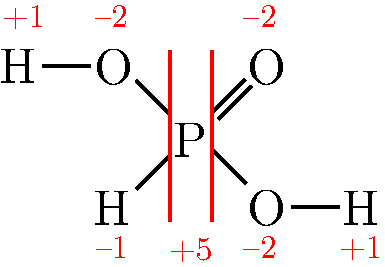
\includegraphics[width=3cm]{figs/valence_and_oxidation_state/phosphorous_acid.pdf}
        \end{figure}
    \end{sol}
\end{problem}

\begin{problem}{}{valence_and_oxidation_state10}
    $\bigstar$ Химический элемент празеодим (Pr) образует несколько устойчивых оксидов, например, оксиды \ce{Pr5O9}, \ce{Pr6O11} и \ce{Pr7O12}. Эти оксиды являются смешанными, так же, как и \ce{Fe3O4}. Предположите состав этих оксидов, учитывая, что празеодим в соединениях проявляет степень окисления $+3$ и $+4$.
    \begin{sol}{\ref{prob:valence_and_oxidation_state10}}
        Двум основным степеням окисления празеодима соответствуют два оксида: \ce{Pr2O3} и \ce{PrO2}, из которых, очевидно, и состоят смешанные оксиды. Все смешанные оксиды с нечётным числом атомов кислорода содержат один или три моль оксида \ce{Pr2O3}. Поэтому для первых двух оксидов очевидно, что
        \begin{equation*}
            \ce{Pr5O9} = 3\ce{PrO2} \cdot \ce{Pr2O3},
        \end{equation*}
        \begin{equation*}
            \ce{Pr6O11} = 4\ce{PrO2} \cdot \ce{Pr2O3}.
        \end{equation*} 
        В оксиде \ce{Pr7O12} чётное число атомов кислорода, поэтому содержится 0 или 2 моль \ce{Pr2O3}, однако отсутствовать в составе он не может, поскольку этот оксид, согласно формуле, не может состоять только из \ce{PrO2}. Значит, в составе 2 моль \ce{Pr2O3}, остальное \ce{PrO2}, т.~е.
        \begin{equation*}
            \ce{Pr7O12} = 3\ce{PrO2} \cdot 2\ce{Pr2O3}.
        \end{equation*}
    \end{sol}
\end{problem}

\clearpage

\section{Аллотропия и полиморфизм}

\hspace*{\parindent}\textbf{Аллотр\'{о}пией}\label{term:allotropy}\index{аллотропия} называют способность одного химического элемента существовать в виде нескольких \emph{простых веществ} с разной формой организации вещества. Аллотропы известны примерно у половины всех химических элементов.

Например, сера имеет две кристаллические аллотропные модификации (существующие в виде молекулярных кристаллов): ромбическую (\ce{\alpha-S}) и моноклинную (\ce{\beta-S}), первая переходит во вторую при температуре \qty{95,5}{\degreeCelsius} (рис.~\ref{fig:rhombic_and_monoclinic_sulfur}).

\begin{figure}[htbp]
    \centering
    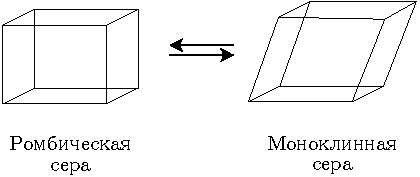
\includegraphics[width=6cm]{figs/allotropy/rhombic_and_monoclinic_sulfur.pdf}
    \caption{Ромбическая и моноклинная сера.}
    \label{fig:rhombic_and_monoclinic_sulfur}
\end{figure}

Кристаллы обеих форм имеют в узлах молекулы \ce{S8} в форме короны (рис.~\ref{fig:S8}).

\begin{figure}[htbp]
    \centering
    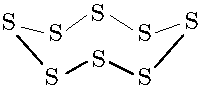
\includegraphics[width=3cm]{figs/allotropy/S8.pdf}
    \caption{Молекула \ce{S8}.}
    \label{fig:S8}
\end{figure}

Также сера имеет аморфную модификацию под названием \emph{пластическая сера} (рис.~\ref{fig:plastic_sulfur}), состоящую из цепочек атомов. Эта модификация образуется при резком охлаждении расплава серы (например, если вылить его в холодную воду) и неустойчива. Со временем она снова превращается в молекулярный кристалл.

\begin{figure}[htbp]
    \centering
    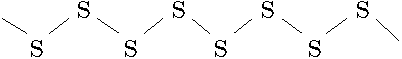
\includegraphics[width=6cm]{figs/allotropy/plastic_sulfur.pdf}
    \caption{Цепочечное строение пластической серы.}
    \label{fig:plastic_sulfur}
\end{figure}

Известными аллотропными модификациями кислорода являются собственно \emph{кислород} \ce{O2} и \emph{озон} \ce{O3}, образующийся в результате действия на кислород искрового разряда. Озон представляет собой менее устойчивую форму и поэтому химически значительно активнее кислорода.

Также широко известны аллотропные модификации фосфора: менее устойчивый \emph{белый фосфор}, состоящий из молекул \ce{P4}, и более устойчивый \emph{красный фосфор} (обозначают \ce{P}).

Аллотропные модификации, как правило, обладают разными физическими и химическими свойствами вследствие их различного строения и стабильности.

Аллотропы обозначают строчными буквами греческого алфавита в порядке возрастания температуры устойчивости. Например, именно \emph{ромбическая сера} получила обозначение \ce{\alpha-S} как устойчивая при более низкой температуре, нежели \emph{моноклинная} сера \ce{\beta-S}.

\subsection*{Полиморфизм}

Аллотропия частично пересекается с \textbf{полиморфизмом}\label{term:polymorphism}\index{полиморфизм}, который распространяется только на твёрдые тела, но зато не только на простые, но и на сложные вещества.

К примеру, карбонат кальция \ce{CaCO3} имеет три полиморфа:

\begin{itemize}
    \item Кальцит (тригональная ячейка);
    \item Арагонит (ромбическая ячейка);
    \item Фатерит (гексагональная форма).
\end{itemize}

Таким образом, аллотропия~--- это частный случай полиморфизма для твёрдых веществ\footnote{В начале XX~века некоторые учёные предлагали отказаться от термина <<аллотропия>> и объединить указанные явления под общим словом <<полиморфизм>>. Однако ничего не вышло: оба термина так и продолжают использоваться.}.

Чтобы лучше продемонстрировать связь аллотропии и полиморфизма, составим табл.~\ref{tab:allotropy_and_polymorphism}.

\begin{table}[htbp]
    \small
    \caption{Аллотропия и полиморфизм.}
    \label{tab:allotropy_and_polymorphism}
    \begin{tabularx}{\textwidth}{
        >{\hsize=1\hsize}Y
        >{\hsize=1\hsize}Y
        >{\hsize=1\hsize}Y
        }
        \hline
        \rowcolor{green!5}
         & Аллотропия & Полиморфизм \\
        \hline
        Область применения & Только химические\newline элементы & Любые \emph{твёрдые} вещества \\
        \hline
        В чём различие форм & Разное строение молекул, тип связи и организации вещества & Разная организация\newline вещества \\
        \hline
        Агрегатное состояние & Любое & Только твёрдое \\
        \hline
        Примеры & \ce{C}: алмаз, графит & \ce{SiO2}: $\alpha$-кварц, $\beta$-кварц, тридимит, кристобалит, коэсит, стишовит \\
        \hline
    \end{tabularx}
\end{table}


\subsection*{Оловянная чума}

\begin{quote}
    \textit{В 1812~году оловянные пуговицы на мундирах солдат Наполеона начали рассыпаться в мороз.}
\end{quote}

\begin{quote}
    \textit{В 1912~году одной из причин гибели экспедиции Роберта Скотта, пытавшейся достичь Южного полюса, стала утечка топлива из баков.}
\end{quote}

\begin{quote}
    \textit{В 1917~году в России многие музейные экспонаты саморазрушились в неотапливаемых помещениях.}
\end{quote}

Что общего между всеми этими событиями? Во всех трёх случаях причиной послужило отсутствие знаний об аллотропных модификациях \emph{олова}.

Олово имеет две наиболее известные модификации: \emph{белое олово} (\ce{\alpha-Sn})~--- тот самый серебристый металл, к которому мы привыкли в фигурках оловянных солдатиков, и в палочках припоя,~--- и \emph{серое олово} (\ce{\beta-Sn}), представляющее собой рыхлый тёмно-серый порошок.

Серое олово не имеет никакой прочности, а переход белого олова в серое сопровождается резким увеличением объёма, что приводит к разрушению изделий.

Как следует из греческих букв в обозначениях аллотропов, серое олово более устойчиво при низких температурах. Переход белого олова в серое начинается при температуре ниже \qty[retain-explicit-plus]{+13,2}{\degreeCelsius}, но происходит постепенно.

При этом даже небольшая затравка серого олова может вызвать резкое ускорение перехода и быстрое разрушение изделий; именно это явление и получило название <<\emph{оловянной чумы}>>.

\begin{problem}{}{allotropy1}
    Какие из следующих веществ являются аллотропными модификациями углерода:
    \begin{itemize}
        \item метан (\ce{CH4});
        \item алмаз;
        \item графит;
        \item угарный газ (\ce{CO});
        \item фуллерен (\ce{C60})?
    \end{itemize}
    Если не знаете про то или иное вещество, изучите информацию о нём в интернет-источниках.
    \begin{sol}{\ref{prob:allotropy1}}
        Аллотропами не могут быть сложные вещества (метан и угарный газ). Остальные вещества~--- это аллотропные модификации углерода.
    \end{sol}
\end{problem}

\begin{problem}{}{allotropy2}
    Почему ромбическая сера плавает на поверхности воды, хотя её плотность значительно выше (\qty{2,07}{\g\per\cm\cubed})?
    \begin{sol}{\ref{prob:allotropy2}}
        Ромбическая сера плавает на поверхности воды из‑за гидрофобности~--- её поверхность не смачивается водой. Кроме того имеются воздушные прослойки между кристаллами, создающие эффект <<поплавка>>.
    \end{sol}
\end{problem}

\begin{problem}{}{allotropy3}
    Олово в последнее время всё реже используется, однако изделия из него всё ещё можно встретить. Подумайте над тем, как можно было бы защититься от <<оловянной чумы>>?
    \begin{sol}{\ref{prob:allotropy3}}
        Самое простое~--- это использовать легирующие добавки, которые затрудняют переход аллотропных форм. Например, очень часто в качестве добавки к олову используется сурьма в составе сплава \textbf{пьютер} (\qty{95}{\percent} \ce{Sn}, \qty{3}{\percent} \ce{Sb}, \qty{2}{\percent} \ce{Cu}). Современные оловянные статуэтки чаще всего изготовлены именно из этого сплава.

        Также можно использовать классические покрытия (лаки, гальванические) или тщательно контролировать условия эксплуатации оловянных изделий.
    \end{sol}
\end{problem}

\begin{problem}{}{allotropy4}
    $\bigstar$ В лаборатории сожгли по \qty{1}{\g} графита и алмаза в избытке кислорода и собрали полученный углекислый газ (\ce{CO2}). Ответьте на два вопроса:
    \begin{enumerate}[label=\arabic*)]
        \item Одинаковый или разный объём углекислого газа образовался?
        \item Одинаковое или разное количество теплоты выделилось при горении?
    \end{enumerate}
    \begin{sol}{\ref{prob:allotropy4}}
        \begin{enumerate}[label=\arabic*)]
            \item В углекислый газ перешло одинаковое количество атомов углерода (масса образцов одинакова), поэтому объём образующегося углекислого газа будет равным.
            \item Количество теплоты будет отличаться (при сгорании алмаза выделяется больше). Графит устойчивее алмаза (именно поэтому эта форма и преобладает на Земле), поэтому при сгорании алмаза будет дополнительно выделяться энергия.
            
            Представьте это как выделение энергии при переходе алмаз $\to$ графит и последующее сгорание обоих образцов графита с выделением одинакового количества энергии.
        \end{enumerate}
    \end{sol}
\end{problem}

\clearpage

\section{Номенклатура бинарных соединений}\label{sec:nomenclature_of_binary_compounds}

\hspace*{\parindent}Самые простые химические соединения, которые образуются при взаимодействии атомов двух \emph{разных} элементов, называют \textbf{бинарными соединениями}\label{term:binary_compounds}\label{бинарные соединения}. Примеры таких соединений:

\begin{equation*}
    \ce{H2O, CS2, HCl, H2S, P2O5, FeS}.
\end{equation*}

Химические свойства и формы организации вещества бинарных соединений очень разнообразны и зависят от того, какими элементами они образованы. В этом разделе мы рассмотрим правила научной номенлатуры бинарных соединений, потому что именно она лежит в основе правил для составления названий более сложных соединений.

\subsection*{Немного о номенклатурах}

Как вы уже поняли, вопрос номенклатуры является одним из краеугольных камней в химии и является довольно запутанным в связи с богатым историческим прошлым и многообразием веществ. И в настоящее время одно и то же соединение можно называть по разному в зависимости от того, какая номенклатура будет использована. Вы будете постоянно встречаться с этим явлением в своей карьере химика и единственный способ избежать недоразумений~--- это разобраться в тонкостях \emph{каждой} номенклатуры.

В общем случае существует набор \textbf{систематических}\label{term:systematic_nomenclature}\index{систематическая номенклатура} номенклатур (ИЮПАК), \textbf{заместительная}\label{term:substitution_nomenclature}\index{заместительная номенклатура} (рациональная) номенклатура, применяющаяся, в основном, для органических соединений и устаревшая \textbf{тривиальная}\label{term:trivial nomenclature}\index{тривиальная номенклатура} номенклатура.

В \emph{Систематических} номенклатурах используется принцип <<одно вещество~--- одно название>>, а также единые правила построения названий для всех классов соединений. Тем не менее, для сложных соединений она может быть довольно неудобной из-за длинных названий.

\emph{Заместительная номенклатура} появилась в середине XIX века и, хотя и опирается на научную систематику (то есть название отражает строение), соединения в ней могут иметь несколько разных названий.

\emph{Тривиальная номенклатура} самая старая и разобщённая, в ней вообще нет никакой системы, а есть просто множество не связанных друг с другом названий отдельных соединений или даже смесей соединений. Названия эти приходится просто запоминать и по самому названию вообще невозможно понять, что за вещество перед нами. Вот вам пример некоторых тривиальных названий:

\begin{itemize}
    \item \textit{Зелень Шееле}~--- \ce{CuHAsO3};
    \item \textit{Медный купорос}~--- \ce{CuSO4*5H2O};
    \item \textit{Халькопирит}~--- \ce{CuFeS2}, оно же <<золото дураков>>;
    \item \textit{Едкий натр}~--- \ce{NaOH}.
\end{itemize}

Тривиальные названия присваивались веществам по внешнему виду, особенностям применения, имени первооткрывателя либо ещё чему годно. Зачастую они проще для запоминания и легче произносятся, чем систематические названия и именно поэтому они до сих пор распространены. Ответ на вопрос <<Нужно ли учить тривиальные названия соединений?>>~--- да, нужно, но только для самых распространённых веществ.


Для названий бинарных соединений наиболее подходящими являются номенклатура Stock и стехиометрическая (умножающая) номенклатура. Также для многих бинарных соединений имеются тривиальные названия. 

\subsection*{Номенклатура Stock}

Эта номенклатура была разработана в начале XX века немецким химиком Альфредом Стоком (\textit{Alfred Stock}). Она ориентируется на указание названий с учётом валентности\footnote{На самом деле с учётом не валентности, а \emph{степени окисления} элементов. Мы будем изучать степень окисления позже, а пока можно с оговорками заменить её на валентность.} химических элементов в соединении.

В бинарных соединениях можно выделить \textbf{электроотрицательную часть}: это элемент, который проявляет б\'{о}льшую \hyperref[sec:electronegativity]{электроотрицательность} и \textbf{электроположительную часть}~--- это элемент с меньшей электроотрицательностью. Формулы бинарных соединений (да и вообще всех соединений) правильно записывать так, чтобы в начале шла электроположительная часть, а затем электроотрицательная. В следующих примерах электроотрицательная часть выделена цветом:

\begin{equation*}
    \ce{P}\textcolor{blue}{\ce{Cl3}}, \ce{Ca}\textcolor{blue}{\ce{H2}}, \ce{Na}\textcolor{blue}{\ce{Cl}}, \ce{Si}\textcolor{blue}{\ce{H4}}.
\end{equation*}

Электроотрицательный элемент даёт название \emph{классу} бинарных соединений, например: хлориды, сульфиды, карбиды. Строится название класса следующим образом:

\begin{equation*}
    \text{\textit{корень из латинского названия}} + \text{-ид}.
\end{equation*}

Необходимые корни латинских названий элементов выделены цветом в таблице химических элементов в приложении~\ref{appendix:Russian_and_Latin_names_of_chemical_elements}. Составим таким образом названия для некоторых классов соединений:

\begin{itemize}
    \item \ce{H}: \textit{\textcolor{blue}{Hydr}ogenium}~--- гидр + -ид $\rightsquigarrow$ гидрид,
    \item \ce{O}: \textit{\textcolor{blue}{Oxy}genium}~--- окс + -ид $\rightsquigarrow$ оксид,
    \item \ce{C}: \textit{\textcolor{blue}{Carb}oneum}~--- карб + -ид $\rightsquigarrow$ карбид,
    \item \ce{N}: \textit{\textcolor{blue}{Nitr}ogenium}~--- нитр + -ид $\rightsquigarrow$ нитрид,
    \item \ce{S}: \textit{\textcolor{blue}{Sulf}ur}~--- сульф + -ид $\rightsquigarrow$ сульфид,
    \item \ce{As}: \textit{\textcolor{blue}{Arsen}icum}~--- арсен + -ид $\rightsquigarrow$ арсенид.
\end{itemize}

Теперь, если прибавить к получившемуся слову название элемента из электроположительной части в родительном падеже, то получим название бинарного соединения:

\begin{itemize}
    \item \ce{CaC2}: карбид кальция,
    \item \ce{HCl}: хлорид водорода,
    \item \ce{KBr}: бромид калия,
    \item \ce{NaH}: гидрид натрия,
    \item \ce{Mg2Si}: силицид магния.
\end{itemize}

Если элемент из электроположительной части может проявлять разную валентность (степень окисления), то чтобы по названию можно было составить правильно формулу, валентность указывают в конце названия в скобках:

\begin{itemize}
    \item \ce{SnO}: оксид олова (II),
    \item \ce{SnO2}: оксид олова (IV),
    \item \ce{PCl3}: хлорид фосфора (III),
    \item \ce{PCl5}: хлорид фосфора (V).
\end{itemize}

Встречаются соединения, в которых атомы электроотрицательной части кроме связей с атомами электроположительной части, образуют также связи между собой (рис.~\ref{fig:hydrazine_peroxide_superoxide}). Такие соединения получают приставку <<\text{пер-}>> к названию класса либо имеют отдельные названия, например:

\begin{itemize}
    \item \ce{H2O2}: пероксид водорода,
    \item \ce{Na2O2}: пероксид натрия,
    \item \ce{KO2}: надпероксид калия,
    \item \ce{N2H4}: гидразин,
    \item \ce{KO3}: озонид калия.
\end{itemize}

\begin{figure}[htbp]
    \centering
    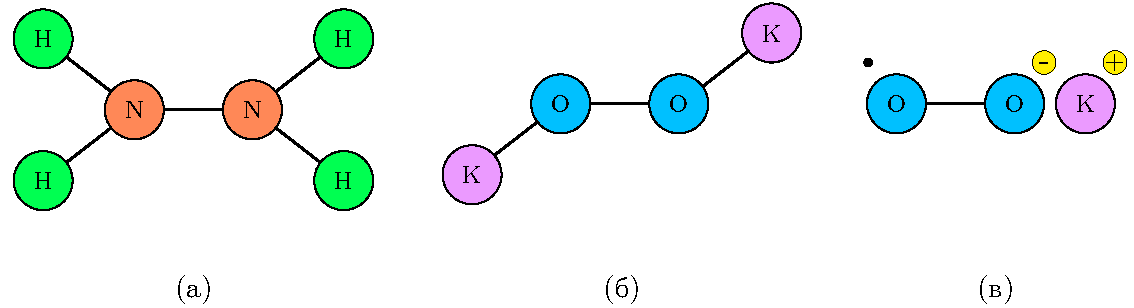
\includegraphics[width=10cm]{figs/nomenclature_of_binary_compounds/hydrazine_peroxide_superoxide.pdf}
    \caption{Образование связей в веществах: гидразин (а), пероксид калия (б), надпероксид калия (в).}
    \label{fig:hydrazine_peroxide_superoxide}
\end{figure}

Не всегда формально правильные названия с приставкой <<\text{пер-}>> имеют устоявшееся употребление. Например, соединение \ce{P2H4} называют не перфосфид водорода, а дифосфан.

Названия классов бинарных соединений с примерами, в том числе для групп с особыми названиями, приведены в приложении~\ref{appendix:names_of_classes_of_binary_compounds}.

\subsection*{Стехиометрическая (умножающая) номенклатура}

Рассмотрим соединение \ce{S2Cl2}, имеющее структуру \ce{Cl-S-S-Cl}. Его название по системе Stock (хлорид серы(I)) совершенно неинформативно, поскольку в данном случае степень окисления, которая равна +1, не совпадает с валентностью атома серы, которая равна двум. Хлорид серы (I) соответствует формуле \ce{SCl}, а не \ce{S2Cl2}. Для соединений такого типа лучше использовать \emph{стехиометрическую номенклатуру}.

В этой номенклатуре название бинарного соединения строят так же, как в номенклатуре Stock, но вместо степени окисления (валентности) греческими приставками указывают количество атомов, например:

\begin{itemize}
    \item \ce{CO}: монооксид углерода,
    \item \ce{PCl3}: трихлорид фосфора,
    \item \ce{Fe3O4}: тетраоксид трижелеза,
    \item \ce{N2O5}: пентаоксид диазота.
\end{itemize}

Соответственно, \ce{S2Cl2} по стехиометрической номенклатуре будет называться дихлорид дисеры.

\begin{problem}{}{nomenclature_of_binary_compounds1}
    Назовите следующие соединения:
    \begin{itemize}
        \item \ce{AlN};
        \item \ce{CaO};
        \item \ce{FeS};
        \item \ce{HF}.
    \end{itemize}
    \begin{sol}{\ref{prob:nomenclature_of_binary_compounds1}}
        Названия соединений:
        \begin{itemize}
            \item нитрид алюминия;
            \item оксид кальция;
            \item сульфид железа (II);
            \item фторид водорода.
        \end{itemize}
    \end{sol}
\end{problem}

\begin{problem}{}{nomenclature_of_binary_compounds2}
    Напишите формулы соединений:
    \begin{itemize}
        \item фторид серы (VI);
        \item селенид цинка;
        \item хлорид бария;
        \item сульфид кадмия.
    \end{itemize}
    \begin{sol}{\ref{prob:nomenclature_of_binary_compounds2}}
        Формулы соединений:
        \begin{itemize}
            \item \ce{SF6};
            \item \ce{ZnSe};
            \item \ce{BaCl2};
            \item \ce{CdS}.
        \end{itemize}
    \end{sol}
\end{problem}

\begin{problem}{}{nomenclature_of_binary_compounds3}
    Назовите следующие соединения:
    \begin{itemize}
        \item \ce{PbH4};
        \item \ce{K2C2};
        \item \ce{Na2S2}.
    \end{itemize}
    \begin{sol}{\ref{prob:nomenclature_of_binary_compounds3}}
        Названия соединений:
        \begin{itemize}
            \item гидрид свинца (IV) (плюмбан);
            \item ацетилид калия;
            \item дисульфид динатрия.
        \end{itemize}
    \end{sol}
\end{problem}

\begin{problem}{}{nomenclature_of_binary_compounds4}
    Напишите формулы соединений:
    \begin{itemize}
        \item дисульфан;
        \item хлорид серы (II);
        \item антимонид лития.
    \end{itemize}
    \begin{sol}{\ref{prob:nomenclature_of_binary_compounds4}}
        Формулы соединений:
        \begin{itemize}
            \item \ce{H2S2};
            \item \ce{SCl2};
            \item \ce{Li3Sb}.
        \end{itemize}
    \end{sol}
\end{problem}

\begin{problem}{}{nomenclature_of_binary_compounds5}
    $\bigstar$ \emph{Профессор Недоумелкин} предложил вам исследовать содержимое сундука, который он обнаружил в подвале дома своей бабушки. В сундуке обнаружились несколько склянок с химическими веществами. Этикетки на них сохранились лишь частично: на них записаны только совершенно непонятные названия и загадочные приписки владельца. Используя информацию в интернете, помогите профессору идентифицировать вещества, чтобы понять, как их использховать и как с ними безопасно обращаться. Итак, надписи на склянках:
    \begin{enumerate}[label=\arabic*)]
        \item \textit{Склянка А}: <<Едкий натр>>. Приписка: <<Осторожно! Превращает жир в мыло, а кожу~--- в язвы. Хранить в сухом месте, ибо тянет влагу из воздуха>>.
        \item \textit{Склянка Б}: <<Медный купорос>>. Приписка: <<Синие слезы. При прокаливании белеет, но при добавлении воды вновь синеет. Яд для грибка>>.
        \item \textit{Склянка В}: <<Нашатырь>>. Приписка: <<Получен из сажи и мочи (по старинному рецепту). При растирании с известью дает удушливый запах>>.
        \item \textit{Склянка Г}: <<Поташ>>. Приписка: <<Добывается из золы сожженных дубовых поленьев. Делает воду мягкой>>.
        \item \textit{Склянка Д}: <<Ляпис>>. Приписка: <<Адский камень. На свету чернеет. Оставляет несмываемые черные метки на коже>>.
    \end{enumerate}
    В углу сундука нашли еще одну бутылку с надписью <<Нашатырный спирт>>. Профессор перепутал её со склянкой \textit{В} (<<Нашатырь>>). Что это за вещества? Почему поташ имеет такое название? Почему ляпис нужно хранить в тёмной посуде?
    \begin{sol}{\ref{prob:nomenclature_of_binary_compounds5}}
        По тривиальным названиям находим информацию о веществах:

        \begin{table}[htbp]
            \small
            \begin{tabularx}{\textwidth}{
                >{\hsize=0.5\hsize}Y
                >{\hsize=1.3\hsize}Y
                >{\hsize=1.4\hsize}Y
                >{\hsize=0.8\hsize}Y
                }
                \hline
                \rowcolor{green!5}
                Склянка & Тривиальное название & Современное название & Формула \\
                \hline
                А & Едкий натр & Гидроксид натрия & \ce{NaOH} \\
                \hline
                Б & Медный купорос & Пентагидрат сульфата меди & \ce{CuSO4*5H2O} \\
                \hline
                В & Нашатырь & Хлорид аммония & \ce{NH4Cl} \\
                \hline
                Г & Поташ & Карбонат калия & \ce{K2CO3} \\
                \hline
                Д & Ляпис & Нитрат серебра & \ce{AgNO3} \\
                \hline
                Е & Нашатырный спирт & Водный раствор аммиака & \ce{NH3*H2O} \\
                \hline
            \end{tabularx}
        \end{table}

        Название <<поташ>> происходит от технологии получения. Золу (богатую карбонатом калия) замачивали в воде, полученный раствор выпаривали в котлах (от англ. <<\textit{pot ash}>>~--- зола из горшка). В результате на стенках котлов кристаллизовался белый налет~--- карбонат калия. Поташ затем использовали в производстве мыла и моющих средств.

        Нитрат серебра фоточувствителен. Под действием света он восстанавливается до металлического серебра, которое имеет черный цвет в порошкообразном состоянии. Поэтому его необходимо хранить, защищая от воздействия света.
    \end{sol}
\end{problem}

\clearpage

\section{Массы в химии}

\begin{wrapfigure}{l}{0.35\textwidth}
    \centering
    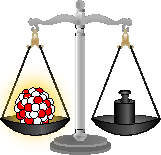
\includegraphics[width=4cm]{figs/atomic_masses/scales.pdf}
\end{wrapfigure}

\hspace*{\parindent}В химии понятие о единицах массы для новичков считается довольно запутанным, поскольку их довольно много и нужно хорошо понимать, в каких случаях необходимо использовать ту или иную единицу. Более того, даже опытные химики частенько путают эти единицы или применяют их неправильно.

Ключ к грамотному использованию каждой единицы~--- это понимание причин, которые побудили их ввести.

У вас уже достаточно знаний, чтобы выстроить атомы в порядке возрастания их массы. Для этого достаточно использовать \hyperref[sec:nuclear_numbers]{массовое число} $A$.

Напомним, что массовое число $A$ равно общему количеству протонов и нейтронов в ядре. Однако точная масса атома не может быть выражена через массовое число и вот почему:

\begin{itemize}
    \item в атоме кроме нуклонов, имеются также электроны, которые тоже имеют некоторую массу;
    \item массы протона и нейтрона немного отличаются;
    \item суммарная масса протонов и нейтронов в ядре немного меньше, чем сумма масс протонов и нейтронов, взятых по отдельности. Это происходит потому, что между нуклонами имеются силы взаимодействия с высокой энергией, связывающие их вместе. Происходит потеря массы согласно уравнению $E = mc^2$. Это явление называют \textbf{дефектом массы}\label{term:mass_defect}\index{дефект массы};
    \item в природе химические элементы редко представлены одним изотопом. Обычно они представляют собой смесь различных изотопов, которые имеют разные массы из-за разного числа нейтронов. Кроме того, изотопный состав веществ на Земле не является постоянным и зависит от места и обстоятельств получения образца. Например, образец углерода, полученный из живых организмов, содержит больше изотопа \ce{^14C}, чем ископаемый углерод.
\end{itemize}

Поэтому в науке используются более пригодные на практике единицы измерения массы атома и химических соединений, каждая из которых служит определённым целям.

\subsection*{Атомная масса $m_a$}

Базовой единицей является \textbf{атомная масса}\label{term:atomic_mass}\index{атомная масса}, которая обозначается $m_a$. Она равна отношению массы атома некоторого элемента \ce{E} к $\frac{1}{12}$ массы изотопа \ce{^12C}:

\begin{equation*}
    m_a(\ce{E}) = \frac{12 \cdot m(\ce{E})}{m(\ce{^12C})}.
\end{equation*}

То есть $\frac{1}{12}$ массы изотопа \ce{^12C} является стандартном атомной массы. Эта величина называется \textbf{атомной единицей массы}\label{term:atomic_mass_constant}\index{атомная единица массы} и обозначается $m_u$.

Другое её название~--- \textbf{углеродная единица}\label{term:carbon_unit}\index{углеродная единица}, что отражает химический элемент, взятый за её основу. Раньше основой для этой единицы служил кислород, и единица называлась кислородной.

Масса углеродной единицы $m_u$ получила обозначение дальтон (Да)\footnote{$\qty{1}{Da} = \qty{1,66053906892(52)e-27}{\kg}$.}. Таким образом, атомная масса изотопа \ce{^12C} равна ровно \qty{12}{\Da}.

Все изотопы, кроме \ce{^12C}, имеют дробные атомные массы по причинам, описанным выше. Однако они довольно близки к целым числам, потому что изменение массы довольно невелико. Округлив атомную массу $m_a$ до ближайшего целого числа, мы получим массовое число $A$ для этого атома. Например, атомная масса изотопа \ce{^63Cu} составляет \qty{62,929}{\Da}, атомная масса изотопа \ce{^28Si}~--- \qty{27,977}{\Da}.

Обратите внимание, что атомная масса может быть использована только для конкретного изотопа и не может быть применена к образцам вещества~--- то есть к смесям большого числа атомов.

\subsection*{Почему отказались от кислородной единицы}

Углеродная единица как единица измерения массы атома была принята с 1960-х годов. До этого существовала похожая на неё \textbf{кислородная единица}.

Переход на углеродную единицу был официально утверждён Международным союзом теоретической и прикладной химии (IUPAC) и Международным союзом теоретической и прикладной физики (IUPAP) в 1961~году.

Причины перехода были сугубо практическими. Природный кислород состоит из трёх стабильных изотопов: \ce{^16O}, \ce{^17O} и \ce{^18O}. Поэтому атомная масса природного кислорода~--- это среднее значение масс этих изотопов с учётом их количества в веществе. Изотопный состав природного кислорода может варьироваться в зависимости от источника получения образца, что приводило к нестабильным результатам измерения атомных масс.

После открытия изотопов кислорода физики и химики некоторое время использовали разные стандарты. Физики принимали за единицу $\frac{1}{16}$ массы изотопа \ce{^16O}, а химики --- $\frac{1}{16}$ средней массы природного кислорода. Это привело к появлению двух разных шкал атомных масс.

Атомы углерода, особенно изотопа \ce{^12C}, оказались более удобными для точных измерений масс с помощью масс-спектрометрии и других методов. Изотоп \ce{^12C} преобладает в природном углероде (около \qty{98,9}{\percent}), что упрощает стандартизацию. Именно поэтому углеродные единицы заменили кислородные.

\subsection*{Относительные единицы массы}

Химики обычно имеют дело не с конкретными изотопами, а с природными материалами, которые, как правило, представляют собой смесь изотопов. Поэтому были введены несколько других единиц измерения массы, которые можно использовать как с отдельными нуклидами, так и с их смесью~--- так называемые относительные единицы массы. Их три:

\begin{itemize}
    \item относительная атомная масса;
    \item стандартный атомный вес;
    \item относительная молекулярная масса.
\end{itemize}

\textbf{Относительная атомная масса}\label{term:relative_atomic_mass}\index{относительная атомная масса} обозначается $A_r(\ce{E})$ и равна отношению массы атома химического элемента к $m_u$:

\begin{equation*}
    A_r({}^i\ce{E}) = \frac{m_a(\ce{E})}{m_u}.
\end{equation*}

Это безразмерная величина, как и все остальные относительные единицы массы.

Её можно рассчитать для определённого изотопа химического элемента \ce{^$i$E}, либо как среднюю величину для \emph{образца} химического элемента, содержащего смесь изотопов:

\begin{equation*}
    A_r(\ce{E}) = \frac{\sum_{n}^{} x_nm_a(\ce{^$i$E}_n)}{m_u}
\end{equation*}

где $x_n$~--- доля атомов n-го изотопа \ce{^$i$E} в смеси.

Но что делать, если мы не знаем изотопный состав конкретного образца вещества? В таком случае используют \textbf{стандартный атомный вес}\label{term:standard_atomic_weight}\index{стандартный атомный вес} $A_{r}^{\circ}(\ce{E})$, который представляет собой относительную атомную массу образца вещества с учётом среднего (типичного) изотопного распределения на Земле (рис.~\ref{fig:relative_atomic_masses}).

\begin{figure}[htbp]
    \centering
    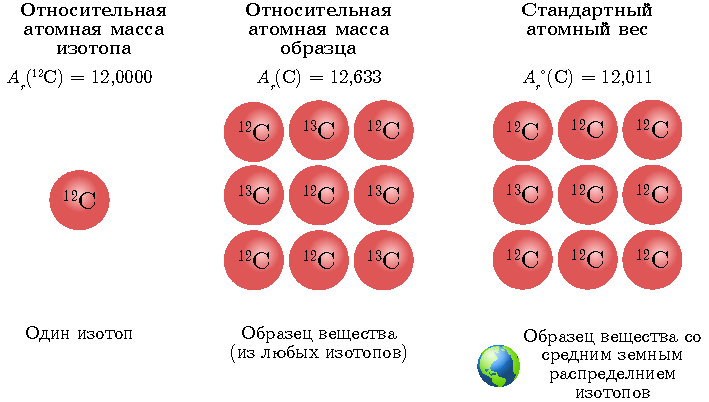
\includegraphics[width=12cm]{figs/atomic_masses/relative_atomic_masses.pdf}
    \caption{Сравнение относительной атомной массы и стандартного атомного веса.}
    \label{fig:relative_atomic_masses}
\end{figure}

Например, известно, что медь представлена на Земле в виде смеси изотопов \ce{^63Cu}, $A_r(\ce{^63Cu}) = \num{62,929}$, составляющего \qty{69}{\percent} всех атомов и \ce{^65Cu}, $A_r(\ce{^65Cu}) = \num{64,927}$, составляющего оставшиеся \qty{31}{\percent}.

За стандартный атомный вес меди, который можно использовать в практических расчётах, принимают

\begin{equation*}
    A_{r}^{\circ}(\ce{Cu}) = \num{0,69} \cdot \num{62,929} + \num{0,31} \cdot \num{64,927} = \num{63,55}.
\end{equation*}

Именно стандартный атомный вес указан в периодической таблице химических элементов.

Сумма относительных атомных масс атомов \emph{в молекуле} называется \textbf{относительной молекулярной массой $M_r$}\label{term:molecular_mass}\index{относительная молекулярная масса}.

Данная величина по сути представляет собой то же самое, что и относительная атомная масса, но относится не к атому или образцу химического элемента, а к химическому соединению.

Рассчитать относительную молекулярную массу просто: нужно сложить относительные атомные массы химических элементов, входящих в молекулу, с учётом их количества в соединении (\ref{eq:molecular_mass}):

\begin{equation}
    \label{eq:molecular_mass}
    M_r({}^{i}\ce{A}_x{}^{j}\ce{B}_y{}^{k}\ce{C}_z) = xA_r({}^{i}\ce{A}) + yA_r({}^{j}\ce{B}) + zA_r({}^{k}\ce{C}).
\end{equation}

Например, для серной кислоты относительная молекулярная масса может быть равна:

\begin{equation*}
    M_r(\ce{^1H2}\ce{^32S}\ce{^16O4}) = 2A_r(\ce{^1H})+A_r(\ce{^32S}) + 4A_r(\ce{^16O}).
\end{equation*}

Если вместо относительных атомных масс использовать стандартный атомный вес элементов, то можно рассчитать относительную молекулярную массу для среднего образца химического соединения на Земле (рис.~\ref{fig:molecular_mass}).

\begin{figure}[htbp]
    \centering
    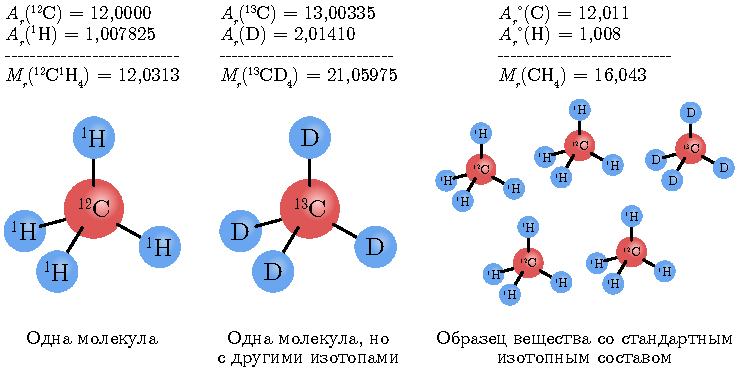
\includegraphics[width=13cm]{figs/atomic_masses/relative_molecular_masses.pdf}
    \caption{Относительная молекулярная масса.}
    \label{fig:molecular_mass}
\end{figure}

\subsection*{Стандартный атомный вес в периодической таблице}

Изучите стандартные атомные веса в \hyperref[appendix:periodic_table]{периодической таблице}. Почему для некоторых элементов они даны с высокой точностью, а для других~--- с довольно низкой? Почему для некоторых элементов стандартный атомный вес вообще не приведён? Давайте разбираться.

Для начала обсудим точность. Некоторые элементы представлены в природе преимущественно в виде одного изотопа и называются \emph{моноизотопными} химическими элементами. Сейчас к ним относят 21 элемент. Это, например, бериллий, натрий, алюминий и пр.\footnote{Вот полный список: \ce{Be}, \ce{Na}, \ce{Al}, \ce{P}, \ce{Sc}, \ce{Mn}, \ce{Co}, \ce{As}, \ce{Y}, \ce{Nb}, \ce{Rh}, \ce{I}, \ce{Cs}, \ce{Pr}, \ce{Tb}, \ce{Ho}, \ce{Tm}, \ce{Lu}, \ce{Au}, \ce{Bi} и \ce{Th}.}

Элементы, которые не являются моноизотопными, представлены смесью изотопов, соотношение которых часто оказывается разным на планете в зависимости от того, из каких источников получен образец. Например, в снегах Антарктиды дейтерия значительно меньше, чем в морской воде.

Для моноизотопных элементов можно указать вес с гораздо большей точностью, чем для остальных, однако такое большое количество значащих цифр обычно не требуется для практического использования\footnote{Если вам нужна высокая точность, то вы можете получить необходимые данные в работе Pure Appl. Chem. 2016; 88(3): 265–291.}. Поэтому стандартный атомный вес в периодической таблице обычно округляют в разумных пределах. Такие веса называют \emph{сокращёнными стандартными атомными весами}\footnote{Например, стандартный атомный вес цезия равен \num{132,90545196(6)}, однако такая точность обычно не нужна, поэтому используют сокращенный вес \num{132,91}.}.

Чем больше различие в изотопном составе какого-либо элемента на планете, тем ниже средняя точность, которую можно использовать для произвольного образца этого элемента, который окажется у вас в руках. Точность, указанная в периодической таблице, равна последней значащей цифре \num{\pm 1}.

Иногда точность хуже, чем \num{\pm 1} последняя значащая цифра, в таком случае её ставят в скобках, например, \num{178,49(2)}.

К примеру, для золота указан стандартный атомный вес равный \num{196,97}, значит, относительная атомная масса образца золота, с которым вы будете иметь дело, скорее всего, окажется в пределах \num{196,96}--\num{196,98}.

Для цинка стандартный атомный вес равен \num{65,38(2)}, значит, истинная относительная атомная масса образца цинка будет лежать в пределах \num{65,36}--\num{65,40}.

Тем не менее, для расчётов берите именно тот атомный вес, который указан в таблице.

Для некоторых элементов рядом со стандартным атомным весом указан знак решётки \#. Например, для кислорода имеется запись \num{15,999}\#. Это означает, что для отдельных образцов, имеющих определённое происхождение, стандартный атомный вес может варьироваться в зависимости от источника образца.

Например, это случается при промышленном производстве некоторых материалов, когда в силу технологического процесса происходит накопление определённых (более лёгких или более тяжёлых) изотопов. Также причиной могут быть многократные фазовые переходы (плавление, испарение), также приводящие к разделению изотопов. При этом в целом на планете состав достаточно стабилен, чтобы использовать указанное значение веса.

К примеру, кислород, содержащийся в воде ледников, будет содержать существенно меньше изотопа \ce{^18O}, чем остальная вода на планете (рис.~\ref{fig:accumulation_of_isotopes_in_nature}).

\begin{figure}[htbp]
    \centering
    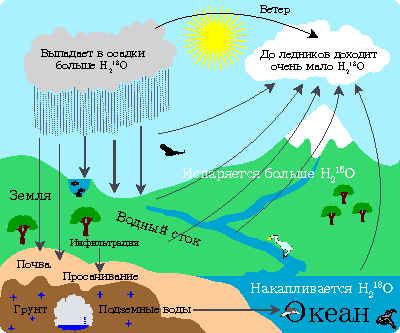
\includegraphics[width=12cm]{figs/atomic_masses/accumulation_of_isotopes_in_nature.pdf}
    \caption{Накопление изотопов кислорода в природе.}
    \label{fig:accumulation_of_isotopes_in_nature}
\end{figure}

Радиоактивные элементы чаще всего имеют настолько непостоянный изотопный состав или настолько малое время жизни, что для них вообще не имеет смысла записывать стандартный атомный вес. В этом случае ограничиваются массовым числом наиболее долгоживущего изотопа и приписывают к нему знак *. К примеру, для радия указано значение 226*.

Тем не менее даже для элементов, не имеющих стабильных изотопов, иногда указывают стандартный атомный вес при условии, что эти элементы обладают больш\'{и}м временем полураспада и имеют более-менее стабильный изотопный состав в земной коре. Это элементы торий, протактиний и уран.

Давайте проверим, как вы усвоили материал. Сформулируйте следующие термины.

\begin{termlist}
    \hyperref[term:mass_defect]{Дефект массы},
    \hyperref[term:atomic_mass]{атомная масса},
    \hyperref[term:atomic_mass_constant]{атомная единица массы}, 
    \hyperref[term:carbon_unit]{углеродная единица},
    \hyperref[term:relative_atomic_mass]{относительная атомная масса},
    \hyperref[term:standard_atomic_weight]{стандартный атомный вес},
    \hyperref[term:molecular_mass]{относительная молекулярная масса}.
\end{termlist}

\begin{problem}{}{atomic_masses1}
    Вы занимаетесь некоторыми научными исследованиями. Какая из величин атомной массы окажется наиболее подходящей в следующих случаях:
    \begin{itemize}
        \item работа в лаборатории синтеза новых соединений;
        \item подбор способов обогащения (выделения) изотопа химического элемента;
        \item исследование возраста археологических останков радиоуглеродным методом;
        \item исследование состава проб грунта океанического дна;
        \item исследование атмосферы Энцелада. 
    \end{itemize}
    \begin{sol}{\ref{prob:atomic_masses1}}
        Выбор зависит от того, имеет значение изотопный состав или нет.
        \begin{itemize}
            \item В лаборатории синтеза обычно пользуются стандартными реактивами, подходит стандартный атомный вес $A_{r}^{\circ}(\ce{E})$.
            \item Если изотопный состав является целью изучения, то можно использовать только относительную атомную массу для образца $A_r(\ce{E})$ либо для конкретного изотопа $A_r({}^i\ce{E})$.
            \item Радиоуглеродный метод использует определение остаточного количества \ce{^14C} по его активности, атомные массы в нём не используются, но если нужны, то достаточно стандартного атомного веса $A_{r}^{\circ}(\ce{E})$.
            \item Исследование химического состава обычно не требует особого внимания к изотопам~--- подходит стандартный атомный вес $A_{r}^{\circ}(\ce{E})$.
            \item На других космических объектах изотопный состав может сильно отличаться от земного и лучше бы его исследовать. Оперируем относительной атомной массой $A_r(\ce{E})$.
        \end{itemize}
    \end{sol}
\end{problem}

\begin{problem}{}{atomic_masses2}
    Во сколько раз в среднем масса атома иода больше массы атома водорода?
    \begin{sol}{\ref{prob:atomic_masses2}}
        В \num{125,9} раз.
    \end{sol}
\end{problem}

\begin{problem}{}{atomic_masses3}
    В \hyperref[appendix:periodic_table]{периодической таблице химических элементов} возможны случаи, когда элементы с б\'{о}льшим стандартным атомным весом стоят раньше элементов с меньшим. Почему это возможно? Приведите примеры таких случаев.
    \begin{sol}{\ref{prob:atomic_masses3}}
        Такие случаи возможны, потому что элементы в периодической таблице располагаются в порядке возрастания зарядового числа $Z$, а не атомных масс, и из-за разнообразия изотопного распределения в природе для отдельных элементов возможна большая доля более тяжёлых изотопов. Примеры таких случаев:

        \begin{table}[htbp]
            \small
            \centering 
            \begin{tabular}{lcc}
                \hline
                \rowcolor{green!5}Элемент & $Z$ & $A_r$ \\
                \hline
                Аргон & 18 & \num{39,948} \\
                Калий & 19 & \num{39,098} \\
                \hline
                Кобальт & 27 & \num{58,933} \\
                Никель & 28 & \num{58,693} \\
                \hline
            \end{tabular}
        \end{table}
    \end{sol}
\end{problem}

\clearpage

\section{Количество вещества. Молярная масса}

\hspace*{\parindent}Теперь, когда мы разобрались с основными единицами атомной массы, давайте разберёмся, как химики оценивают количество вещества.

Дело в том, что мельчайшими носителями \emph{химических свойств} являются именно химические вещества, которые могут представлять из себя довольно различные по сложности и размерам объекты, от простой двухатомной молекулы до огромных белков с массой в десятки тысяч дальтон. При этом в химических реакциях соединения участвуют как единое целое, реагируя друг с другом в пропорциях, кратных количеству частиц.

Именно поэтому в химии недостаточно использования классической массы вещества $m$, а необходимы собственные единицы измерения количества вещества, связанные \emph{с числом частиц}.

При этом от классической массы отказаться невозможно, так как именно с ней мы работаем на практике, когда нам необходимо взять определённое количество вещества.

\subsection*{Количество вещества $n$}\label{term:amount_of_substance}\index{количество вещества}

Итак, нам необходимо перейти от атомных масс к практическим массам в граммах и килограммах, которые используются в работе. При этом нужно ввести ещё одну единицу количества вещества, связанную \emph{с числом частиц} (атомов, молекул, электронов).

Здесь были достигнуты следующие договорённости. За стандарт количества вещества принят образец изотопа \ce{^12C} массой ровно \qty{12}{\g}\footnote{Почему 12? Чтобы сохранить совместимость с прежней кислородной шкалой.}. Количество вещества, содержащее столько же частиц, сколько атомов содержится в этом образце получило название \qty{1}{\mole} вещества.

Таким образом, \textbf{моль}~--- единица измерения количества вещества, опирающаяся на число частиц, а не на их массу, размер и т.~п. Количество вещества в молях принято обозначать буквой $n$.

\subsection*{Молярная масса $M$}

Наконец, завершает <<парад>> единиц измерения массы в химии \textbf{молярная масса}\label{term:molar_mass}\index{молярная масса} вещества. Она представляет собой массу одного моля вещества в граммах или килограммах. По определению, она равна отношению массы вещества к его количеству и выражается в г/моль (\ref{eq:molar_mass}):

\begin{equation}
    \label{eq:molar_mass}
    \fbox{$\displaystyle M = \frac{m}{n}$}.
\end{equation}

Молярная масса может относиться к любым объектам~--- атомам, молекулам и пр., поскольку привязана к числу частиц, которые могут быть какими угодно. Например, молярная масса фтора как элемента $M(\ce{F}) = \qty{19}{\g\per\mole}$, а в виде простого вещества (молекулы \ce{F2})~--- $M(\ce{F2}) = \qty{38}{\g\per\mole}$.

Поскольку моль, так же как и атомные массы, привязан к углеродной единице, то молярная масса, выраженная в г/моль, численно совпадает с относительной молекулярной массой и мы можем спокойно воспользоваться значениями стандартных атомных весов из периодической таблицы для расчёта молярных масс соединений.

Однако надо чётко представлять разницу между молярной массой и относительной молекулярной массой, понимая, что они равны лишь численно и отличаются по размерности.

Молярную массу соединений рассчитывают точно так же, как и относительную молекулярную массу:

\begin{equation*}
    M(\ce{H2SO4}) = 2M(\ce{H})+M(\ce{S}) + 4M(\ce{O}).
\end{equation*}

\subsection*{Число Авогадро $N_A$}

Теперь мы знаем, что в одном моле любого вещества содержится столько же частиц, сколько атомов содержится в \qty{12}{\g} изотопа \ce{^12C}. А сколько это частиц? Оказывается, довольно много: \num{6,02214076e23} атомов. Это число называется \textbf{числом Авогадро}\label{term:Avogadro_constant}\index{число Авогадро} и обозначается $N_A$. Соответственно, можно записать соотношение (\ref{eq:amount_of_substance_in_terms_of_the_number_of_particles}) для определения количества вещества через число частиц:

\begin{equation}
    \label{eq:amount_of_substance_in_terms_of_the_number_of_particles}
    \fbox{$\displaystyle n = \frac{N}{N_A}$}.
\end{equation}

То есть количество вещества можно определить как по массе с использованием молярной массы соединений, так и по количеству частиц $N$ в веществе.

\subsection*{Молярный объём газов}

Но это ещё не всё. Для газов оказалось, что в одинаковых объёмах разных газов при одинаковых условиях содержится одинаковое количество частиц. То есть объём \qty{1}{\mole} любого газа одинаков при определённых условиях (давление и температура). При нормальных условиях\footnote{Нормальными условиями (н.~у.) согласно рекомендациям ИЮПАК 1982~года считаются $T = \qty{273,15}{\K}$ (\qty{0}{\degreeCelsius}), $p = \qty{e5}{\Pa}$ (\qty{101,325}{\kPa}, \qty{1}{\atm}).} этот объем (обозначаемый $V_m$) равен \qty{22,4}{\l\per\mole}\footnote{А если точнее~--- \qty{22,710953}{\l\per\mole}.}. Поэтому мы можем записать и третье соотношение (\ref{eq:amount_of_substance_in_terms_of_volume}) для определения количества вещества:

\begin{equation}
    \label{eq:amount_of_substance_in_terms_of_volume}
    \fbox{$\displaystyle n = \frac{V}{V_m}$}.
\end{equation}

Величину $V_m$ называют \textbf{молярным объёмом газа}\label{term:molar_volume}\index{молярный объём газа}. Нетрудно видеть, что его можно выразить и через плотность газа (в \unit{\g\per\l}):

\begin{equation}
    \label{eq:molar_volume}
    V_m = \frac{V}{n} = \frac{M}{\rho}.
\end{equation}

Подводя итоги этого и предыдущего разделов, составим сводную табл.~(\ref{tab:unit_measurements_of_atomic_masses}) единиц измерения атомных и молекулярных масс.

\begin{table}[htbp]
    \small
    \caption{Единицы измерения атомных масс}
    \label{tab:unit_measurements_of_atomic_masses}
    \begin{tabularx}{\textwidth}{
        >{\hsize=1.2\hsize}Y
        >{\hsize=0.8\hsize}Y
        >{\hsize=0.8\hsize}Y
        >{\hsize=1.2\hsize}Y
        }
        \hline
        \rowcolor{green!5}
        Единица массы & Обозначение & Ед. \newline измерения & Используется для \\
        \hline
        Атомная масса & $m_a$ & Да & один изотоп \\
        \hline
        Относительная \newline изотопная масса & $A_r({}^{i}\ce{E})$ & нет & один изотоп \\
        \hline
        Относительная \newline атомная масса & $A_r(\ce{E})$ & нет & образец вещества \\
        \hline
        Стандартный \newline атомный вес & $A_{r}^{\circ}(\ce{E})$ & нет & типичный образец \newline вещества с Земли \\
        \hline
        Относительная \newline молекулярная масса & $M_r$ & нет & молекула \\
        \hline
        Молярная масса & $M$ & \unit{\g\per\mole} & \qty{1}{\mole} вещества \\
        \hline
    \end{tabularx}
\end{table}

Давайте проверим, как вы усвоили материал. Сформулируйте определения терминов из блока ниже, а затем решите задачи.

\begin{termlist}
    \hyperref[term:amount_of_substance]{Количество вещества},
    \hyperref[term:molar_mass]{молярная масса},
    \hyperref[term:Avogadro_constant]{число Авогадро},
    \hyperref[term:molar_volume]{молярный объём газа}.
\end{termlist}

\begin{problem}{}{unit_measurements_of_atomic_masses1}
    Рассчитайте молярную массу следующих сложных веществ: а) \ce{H2SO4}, б) \ce{H2O}, в) \ce{NaOH}, г) \ce{Ba(OH)2}, д) \ce{Al2(SO4)3}, е) \ce{Na2HPO4}, ж) \ce{KAl(SO4)2*12H2O}, з) \ce{C12H22O11}.  
    \begin{sol}{\ref{prob:unit_measurements_of_atomic_masses1}}
        $M$,~\unit{\g\per\mole}: а) \num{98,08}, б) \num{18,02}, в) \num{40,00}, г) \num{171,36}, д) \num{342,15}, е) \num{141,96}, ж) \num{474,39}, з) \num{342,30}.
    \end{sol}
\end{problem}

\begin{problem}{}{unit_measurements_of_atomic_masses2}
    Какой газ тяжелее: озон (\ce{O3}) или кислород (\ce{O2})?
    Почему озон не скапливается у поверхности земли?  
    \begin{sol}{\ref{prob:unit_measurements_of_atomic_masses2}}
        Согласно формуле \ref{eq:molar_volume} большей плотностью обладает газ с большей молярной массой, то есть озон. Он не скапливается у поверхности земли по описаным ниже причинам.
        \begin{itemize}
            \item Озон --- неустойчивое соединение. Он легко разлагается обратно на кислород под воздействием видимого света, тепла и других факторов. Это препятствует его накоплению в нижних слоях атмосферы.
            \item Турбулентное перемешивание воздуха. В тропосфере (нижнем слое атмосферы) происходит активное перемешивание воздушных масс из-за конвекции, ветра и других метеорологических процессов. Это не позволяет газам разделяться по плотности --- даже более тяжёлым, таким как озон.
            \item Образование в верхних слоях атмосферы. Большая часть озона (около \qty{90}{\percent}) сосредоточена в стратосфере, на высоте от 20 до \qty{40}{\km}. Там он образуется под воздействием ультрафиолетового излучения Солнца из молекулярного кислорода. В этих условиях озон формируется и тут же разлагается в динамическом равновесии, то есть просто не успевает попасть к поверхности.
            \item Температурная инверсия в стратосфере. В стратосфере температура повышается с высотой из-за поглощения озоном ультрафиолетового излучения. Это создаёт барьер (тропопаузу), который затрудняет перемешивание воздуха между тропосферой и стратосферой. Таким образом, озон <<задерживается>> в стратосфере, а не опускается к поверхности Земли.
        \end{itemize}
    \end{sol}
\end{problem}

\clearpage

\section{\# Как взвесили атом}

\hspace*{\parindent}Освоив предыдущий урок, некоторые могут задать вполне логичный вопрос: если известна масса одного моля любого вещества в привычных нам единицах измерения массы, то как изначально определили, какова масса одного атома? Атом не положить на весы, а число Авогадро настолько велико, что буквально потрясает воображение.

Атомы настолько малы, что даже сейчас количественные исследования масс на субатомном уровне, по сути, большая редкость. Как же при уровне технологий начала XX века человек сумел провести такие количественные измерения? Давайте погрузимся немного в историю и выясним, как это произошло и проследим за творческой работой ума исследователей.

К концу XIX века гипотеза о существовании атомов, как носителей свойств веществ уже успешно применялась для объяснения природных явлений: представления о химических реакциях, природы тепла и холода, агрегатного состояния веществ.

Тем не менее, наличие отдельных атомов ещё никому не удалось зафиксировать. Было понятно, что атомы очень малы, но насколько они малы? Каков их размер и масса?

Применяя количественный анализ при химических реакциях, исследователи установили, что атомы различных химических элементов обладают различным весом. 

Постепенно стали известны относительные атомные веса (в сравнении с массой атома водорода) почти всех открытых на тот момент химических элементов. Однако абсолютные значения массы и размера атомов оставались загадкой.

\subsection*{Броуновское движение}

Задолго до возникновения проблемы определения массы атома было открыто так называемое \textbf{броуновское движение}\label{term:Brownian_motion}\index{броуновское движение}, которое впоследствии и помогло в решении этой задачи.

В 1827~году Роберт Броун решил опробовать свой новый микроскоп и рассмотрел каплю воды с частицами очень мелкой цветочной пыльцы. Учёный с удивлением обнаружил, что частицы пыльцы движутся. Движение их было совершенно хаотично, напоминало роение тучи мелких мошек, словно частицы были живые (рис.~\ref{fig:Brownian_motion}).

\begin{figure}
    \centering
    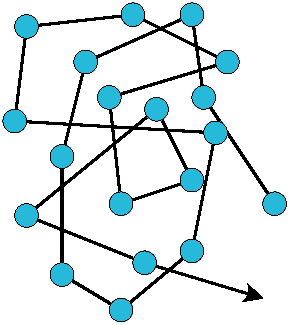
\includegraphics[width=3cm]{figs/how_the_atom_was_weighed/Brownian_motion.pdf}
    \caption{Примерно так выглядят траектории движения частиц пыльцы при броуновском движении.}
    \label{fig:Brownian_motion}
\end{figure}

Однако последующие исследования показали, что частицы не были живыми (такую же картину движения под микроскопом удалось получить даже с табачным дымом), зато выяснилось, что броуновское движение обладало следующими особенностями:

\begin{itemize}
    \item является беспорядочным;
    \item никогда не прекращается;
    \item если наблюдать за частицами очень долго, то в среднем их среднеквадратичное смещение пропорционально времени наблюдения ($\left\langle x^2\right\rangle \varpropto t $);
    \item частицы с размерами больше \qty{5}{\um} не участвуют в броуновском движении.
\end{itemize}

Броуновское движение очевидно было связано с тем, что на частицы действует какая-то сила, причём для мелких мелких частиц статистические флуктуации числа ударов молекул с разных сторон становятся значимыми, создавая неуравновешенную силу, в результате чего частица начинает двигаться или вращаться, а для крупных~--- равномерна со всех сторон, из-за чего силы уравновешиваются и частица не движется.

Данное явление связали с тепловым движением атомов среды, в которой находятся частицы. При движении молекулы среды могут соударяться с частицей, передавая ей часть импульса и заставляя её двигаться. Купные частицы испытывают соударения со всех сторон. При этом сами атомы остаются не видны.

\subsection*{Работы Жана Перрена}

В описанных выше системах микрочастиц, взвешенных в воде, все частицы были разного размера (и массы), что не давало возможности исследовать законы их движения в количественном виде. Поэтому на первом этапе своих работ французский физик Жан Перрен задался целью получить однородные по размерам частицы.

В качестве объекта исследования он использовал гуммигут~--- затвердевшую смолу, получаемую из деревьев семейства гуммигутовых. Частицы гуммигута в воде (суспензию) Перрен подвергал многократному центрифугированию, отделяя частицы определённой массы (и размера), в результате чего через месяц кропотливой работы учёный сумел собрать несколько однородных фракций частиц с размерами \num{0,5}, \num{0,46}, \num{0,37}, \num{0,21} и \qty{0,14}{\um}.

Далее Перрен изготовил стеклянную запаянную кювету высотой \qty{0,1}{\mm}, заполненную водой, в которую помещал частицы из полученных фракций.

\begin{figure}[htbp]
    \centering
    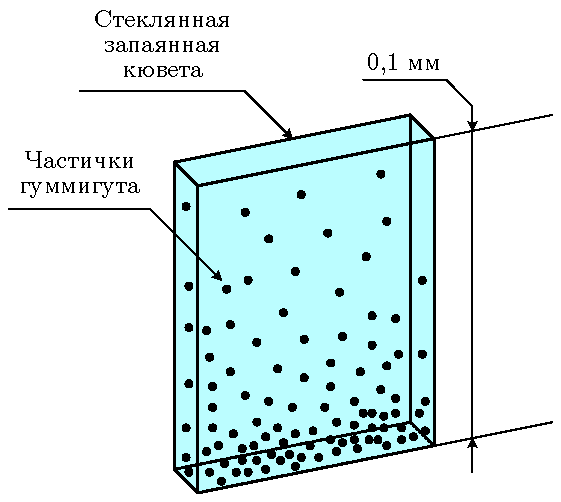
\includegraphics[width=6cm]{figs/how_the_atom_was_weighed/gummigut_cuvette.pdf}
    \caption{Кювета с частичками гуммигута.}
    \label{fig:gummigut_cuvette}
\end{figure}

Вначале частицы равномерно распределялись в кювете, однако постепенно оседали и с течением времени в нижней части кюветы всегда скапливалась основная масса частиц, хотя некоторое количество продолжало оставаться и в верхней части (рис.~\ref{fig:gummigut_cuvette}).

Количество частиц можно было определять при помощи подсчёта под микроскопом. Это оказалось довольно трудоёмко, поскольку частицы всё время двигались, однако Перрен использовал средние значения при многократном подсчёте.

Учёный разделил высоту кюветы на промежутки и рассчитывал число частиц $n$ на каждой из исследуемых высот (за нулевую высоту был принят уровень дна, $n_0$~--- число подсчитанных частиц на нулевой высоте).

Оказалось, что на высоте \qty{35}{\um} частиц было вдвое меньше, чем на высоте \qty{5}{\um}, на высоте \qty{65}{\um}~--- вдвое меньше, чем на \qty{35}{\um}, на высоте \qty{95}{\um}~--- вдвое меньше, чем на \qty{65}{\um} (рис.~\ref{fig:results_of_Perrins_experiment}).

\begin{figure}[htbp]
    \centering
    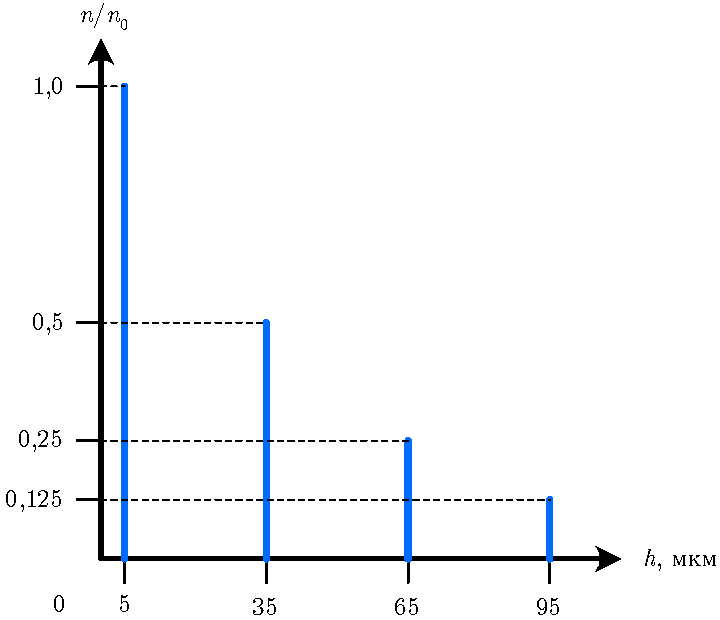
\includegraphics[width=8cm]{figs/how_the_atom_was_weighed/results_of_Perrins_experiment.pdf}
    \caption{Результаты подсчёта числа частиц на различной высоте кюветы.}
    \label{fig:results_of_Perrins_experiment}
\end{figure}

То есть при поднятии вверх на каждые \qty{30}{\um} число частиц уменьшалось вдвое. Увеличение высоты представляло собой арифметическую прогрессию, а уменьшение числа частиц~--- геометрическую. Это было удивительно и привлекало внимание, потому что такая закономерность наблюдалась применительно и к другому объекту: по такому же закону спадает плотность воздуха в атмосфере при увеличении высоты.

Этот закон называется \textbf{барометрической формулой}\label{term:barometric_formula}\index{барометрическая формула} и выглядит следующим образом:

\begin{equation}
    \label{eq:barometric_formula}
    \lg \frac{n_0}{n} = Amg(h - h_0).
\end{equation}

Допустим, на какой-то высоте $h_0$ в каждом кубическом сантиметре содержится $n_0$ молекул газа. Тогда на некоторой большей высоте $h$ будет содержаться $n$ молекул газа. При этом $A$~--- некоторая константа, зависящая от температуры, $m$~--- масса молекулы газа, $g$~--- ускорение свободного падения.

Выберем такую разность высот $h - h_0$, чтобы число частиц стало вдвое меньше. Тогда

\begin{equation*}
    \frac{n_0}{n} = 2,
\end{equation*}

\begin{equation*}
    \lg 2 = Amg(h - h_0).
\end{equation*}

Таким образом, взвесь частиц гуммигута в воде можно представить как распределение молекул в атмосфере, но с той разницей, что вода гораздо более плотная среда, а частицы гуммигута гораздо тяжелее, чем молекулы газа, поэтому это распределение более сжато.

Если бы была известная константа $A$, то измерив высоту, на которой число частиц газа убывает вдвое мы смогли бы вычислить $m$, то есть массу молекулы газа. Однако, она не была известна.

Однако, что, если пойти обратным путём и взвесить частицы гуммигута, которые уже достаточно велики, чтобы определить их массу. Тогда из соотношения (\ref{eq:barometric_formula}) можно рассчитать константу $A$. Поскольку Перрен добился одинаковых размеров для своих фракций частиц, то зная плотность гуммигута он мог рассчитать массу каждой частицы.

При поднятии на каждые \qty{5}{\km} количество кислорода в воздухе уменьшается вдвое. \qty{5}{\km} это в 166 миллион раз больше, чем \qty{30}{\um}. Значит, масса гуммигутовой частицы диаметром \qty{0,21}{\um} также в 166 миллион раз больше, чем молекулы кислорода.

В результате подсчётов (с поправкой на силу Архимеда) масса одного зёрнышка гуммигута у Перрена получилась равной \qty{8,5e-15}{\g}. Значит, масса молекулы кислорода равна \qty{5,1e-23}{\g}. А так как относительная масса молекулы кислорода в 32 раза больше, чем атома водорода (с которым производили сравнение), то масса атома водорода равна \qty{1,6e-24}{\g}. Следовательно, в одном грамме водорода содержится \num{6e23} атомов. Узнаёте это число?

Эти значения позволили связать имевшиеся относительные атомные веса с граммом и ввести понятие количества вещества в молях и молярную массу. Измерения Перрена были не очень точны, однако они впоследствии были уточнены другими, более точными способами. Сейчас мы знаем, что точная масса молекулы кислорода равна \qty{5,314e-23}{\g}, а атома водорода \qty{1,674e-24}{\g}.

\begin{problem}{}{how_the_atom_was_weighed1}
    Используя приведённые выше данные, рассчитайте, при подъёме на какую высоту давление воздуха уменьшится вдвое? Воздух легче кислорода в соотношении $\num{28,8}/32$.
    \begin{sol}{\ref{prob:how_the_atom_was_weighed1}}
        Рассчитаем константу $A$ из барометрической формулы (\ref{eq:barometric_formula}) используя данные для кислорода:

        \begin{equation*}
            A = \frac{\lg 2}{m_{\text{кисл.}}g(h - h_0)} = \frac{\lg 2}{\num{5,3140e-26} \cdot \num{9,81} \cdot \num{5000}} = \qty{1,1549e20}{\s\squared\per\kg\m\squared}.
        \end{equation*}

        Найдём среднюю массу молекулы воздуха:

        \begin{equation*}
            m_{\text{возд.}} = m_{\text{кисл.}} \cdot \frac{\num{28,8}}{32} = \num{5,314e-26} \cdot \frac{\num{28,8}}{32} = \qty{4,6498e-26}{\kg}.
        \end{equation*}

        Наконец, рассчитаем разность высот $(h - h_0)$:

        \begin{equation*}
            (h - h_0) = \frac{\lg 2}{Am_{\text{возд.}}g} = \frac{\lg 2}{\num{1,1549e20} \cdot \num{4,6498e-26} \cdot \num{9,81}} = \qty{5714,3}{\m}.
        \end{equation*}
    \end{sol}
\end{problem}

\begin{problem}{}{how_the_atom_was_weighed2}
    Найдите высоту над уровнем моря, на которой давление воздуха равно \qty{0,25}{\atm}.
    \begin{sol}{\ref{prob:how_the_atom_was_weighed2}}
        В барометрической формуле изменим левую часть уравнения и выразим разницу высот:

        \begin{equation*}
            \lg \frac{n_0}{n} = \lg \frac{1}{\num{0,25}} = Amg(h-h_0)
        \end{equation*}

        \begin{equation*}
            (h-h_0) = \frac{\lg 4}{Amg} = \frac{\lg 4}{\num{1,1549e20} \cdot \num{4,6498e-26} \cdot \num{9,81}} = \qty{11428,6}{\m}.
        \end{equation*}
    \end{sol}
\end{problem}

\clearpage

\section[Основные стехиометрические соотношения. Доли]{Основные стехиометрические соотношения.\\Доли}

Одним из разделов химии, из которого она выросла как количественная наука является \textbf{стехиометрия}\label{term:stoichiometry}\index{стехиометрия}~--- раздел, посвящённый количественным отношениям веществ, вступающих в химическую реакцию. 

Для начала мы изучим основные понятия стехиометрии, а затем, после того, как познакомимся с уравнениями химических реакций, потренируемся в количественных расчётах.

\subsection*{Основные стехиометрические соотношения}

Объединив выражения (\ref{eq:molar_mass}--\ref{eq:molar_volume}) мы можем подвести итоги возможных способов расчёта количества вещества:

\begin{equation}
    \label{eq:stoichiometric_relations}
    \fbox{$\displaystyle n = \frac{m}{M} = \frac{N}{N_A} = \frac{V}{V_m} = \frac{V\rho }{M}$}.
\end{equation}

Из последнего равенства можно вывести выражение (\ref{eq:gas_density}) для расчёта плотности газа:

\begin{equation}
    \label{eq:gas_density}
    \fbox{$\displaystyle \rho = \frac{M}{V_m}$}.
\end{equation}

Соотношения~\ref{eq:stoichiometric_relations} называются \textbf{основными стехиометрическими соотношениями}\label{term:stoichiometric_relations}\index{основные стехиометрические соотношения} и используются химиками постоянно.

\begin{example}{}{ex:stoichiometric_relations1}
    \textit{Сколько моль содержится в \qty{9,008}{\g} чистой воды (\ce{H2O})?}

    \medskip

    \textit{Решение.} Вначале найдём молярную массу воды. Для этого сложим стандартные атомные веса составляющих её элементов с учётом количества атомов в молекуле. Из \hyperref[appendix:periodic_table]{периодической таблицы} находим стандартные атомные веса водорода и кислорода и вычисляем молярную массу воды:

    \begin{equation*}
        A_r(\ce{H}) = \num{1,008}, A_r(\ce{O}) = \num{15,999},
    \end{equation*}

    \begin{equation*}
        M(\ce{H2O}) = 2 \cdot \num{1,008} + \num{15,999} = \qty{18,015}{\g\per\mole}.
    \end{equation*}

    Тогда количество вещества в данной массе воды будет равно:
    \begin{equation*}
        n(\ce{H2O}) = \frac{m_{\ce{H2O}}}{M_{\ce{H2O}}} = \frac{\num{9,008}}{\num{18,015}} = \qty{0,5}{\mole}.
    \end{equation*}
\end{example}

\begin{example}{}{ex:stoichiometric_relations2}
    \textit{Вычислите среднюю массу одного атома серебра в граммах.}

    \medskip

    \textit{Решение.} Стандартный атомный вес серебра равен \num{107,868}. То есть один моль серебра весит \qty{107,868}{\g}. \qty{1}{\mole} любого вещества содержит число Авогадро частиц, то есть \num{6,02e23} частиц, в данном случае атомов. Значит, средняя масса одного атома будет равна:

    \begin{equation*}
        m = \frac{\num{107,868}}{\num{6,02e23}} = \qty{1,79e-22}{\g}.
    \end{equation*}
\end{example}

\begin{example}{}{ex:stoichiometric_relations3}
    \textit{Какова плотность кислорода при н.~у.?}

    \medskip

    \textit{Решение.} Кислород представляет собой двухатомный газ (\ce{O2}), молярная масса которого равна $M(\ce{O2}) = 2M(\ce{O}) = 2 \cdot \num{15,999} = \qty{31,998}{\g\per\mole}$. Пользуясь формулой (\ref{eq:gas_density}) рассчитываем:
    \begin{equation*}
        {\rho}(\ce{O2}) = \frac{M}{V_m} = \frac{\num{31,998}}{\num{22,4}} = \qty{1,428}{\g\per\l}.
    \end{equation*}
\end{example}

\subsection*{Доли}

В химии широко используется понятие \emph{доля}. Эта величина показывает, какую часть составляет тот или иной компонент от общего рассматриваемого объекта. Например, \textbf{мольная доля}\label{term:eq:mole_fraction}\index{мольная доля} $x_i$ показывает, какую часть составляет количество вещества отдельного компонента $i$ от суммы количеств веществ всех компонентов $N$ объекта в молях:

\begin{equation}
    \label{eq:mole_fraction}
    \fbox{$\displaystyle x_i = \frac{n_i}{n_{\text{общ}}} = \frac{n_i}{\sum_{i = 1}^{N} n_i}$},
\end{equation}

где $n_i$~--- количество вещества искомого компонента, $n_{\text{общ}}$~--- сумма количеств веществ всех компонентов в смеси (включая искомый). Сумма мольных долей всех $N$ компонентов равна 1:

\begin{equation*}
    \sum_{i = 1}^{N} x_i = 1.
\end{equation*}

Поскольку в выражении (\ref{eq:mole_fraction}) числитель и знаменатель имеют размерность в молях, мольная доля~--- величина безразмерная. Однако поскольку величина мольной доли может варьироваться от 0 до 1, её часто выражают в процентах.

Точно также вычисляются \textbf{массовая доля}\label{term:mass_fraction}\index{массовая доля} $w_i$ и \textbf{объёмная доля}\label{term:volume_fraction}\index{объёмная доля} ${\varphi}_i $ с той лишь разницей, что вместо количеств веществ используются массы и объёмы компонентов:

\begin{equation}
    \label{eq:mass_fraction}
    \fbox{$\displaystyle w_i = \frac{m_i}{m_{\text{общ}}} = \frac{m_i}{\sum_{i = 1}^{N} m_i}$}.
\end{equation}

\begin{equation}
    \label{eq:volume_fraction}
    \fbox{$\displaystyle {\varphi }_i = \frac{V_i}{V_{\text{общ}}} = \frac{V_i}{\sum_{i = 1}^{N} V_i}$}.
\end{equation}

Понятие доли похоже на понятие \emph{концентрации}, которое мы будем изучать позже. Главное их отличие в том, что в определении концентрации количество компонента в одиних единицах измерения соотносят с количеством целого объекта, выраженного в \emph{других} единицах измерения.

Поэтому величины концентрации всегда имеют размерность, например, \unit{\g\per\l}, \unit{\mole\per\l}, и могут принимать любые значения от нуля до бесконечности, тогда как доли~--- всегда безразмерная величина, лежащая в интервале от 0 (нет в составе) до 1 (полностью состоит из указанного компонента).

\begin{example}{}{ex:stoichiometric_relations4}
    \textit{Рассчитайте мольную долю водорода в азотной кислоте \ce{HNO3}.}

    \medskip

    \textit{Решение.} В молекуле азотной кислоты на один атом водорода приходится один атом азота и три атома кислорода, поэтому, воспользовавшись формулой (\ref{eq:mole_fraction}) рассчитываем:

    \begin{equation*}
        x_{\ce{H}} = \frac{n_{\ce{H}}}{n_{\ce{H}} + n_{\ce{N}} + n_{\ce{O}}} = \frac{1}{1 + 1 + 3} = \num{0,2}.
    \end{equation*}
\end{example}

\begin{example}{}{ex:stoichiometric_relations5}
    \textit{Рассчитайте массовую долю водорода в азотной кислоте.}

    \medskip

    \textit{Решение.} Скомбинируем выражения (\ref{eq:mass_fraction}) и (\ref{eq:stoichiometric_relations}) и выведем выражение для расчёта массовой доли через количества веществ:
    \begin{equation*}
        w_i  = \frac{m_i}{\sum_{i}^{} m_i} = \frac{n_iM_i}{\sum_{j}^{}n_jM_j}.
    \end{equation*}
    Подставляя соотношение атомов в молекуле азотной кислоты и молярные массы элементов в это выражение, находим:
    \begin{equation*}
        w_i  = \frac{\num{1,008}}{1 \cdot \num{1,008} + 1 \cdot \num{14,007} + 3 \cdot \num{15,999}} = \num{0,0159}.
    \end{equation*}
\end{example}

Выведем выражения для связи мольной и массовой долей. Выразим массовую долю через мольную, воспользовавшись выражением из последнего примера:

\begin{equation}
    w_i  = \frac{n_iM_i}{\sum_{i}^{}n_iM_i} = \frac{x_iM_i\sum_{i}^{}n_i}{\sum_{j}^{}\{ x_jM_j\sum_{i}^{}n_i\}} = \frac{x_iM_i}{\sum_{j}^{}x_jM_j}.
\end{equation}

Мольную долю выразим через массовую скомбинировав выражения (\ref{eq:mole_fraction}) и (\ref{eq:mass_fraction}):

\begin{equation}
    \label{eq:mole_fraction_via_mass_fraction}
    x_i = \frac{n_i}{\sum_{i}^{} n_i} = \frac{\frac{m_i}{M_i}}{\sum_{j}^{}\frac{m_j}{M_j}} = \frac{\frac{w_i}{M_i}}{\sum_{j}^{}\frac{w_j}{M_j}}.
\end{equation}

\subsection*{Молярная масса смеси}\label{term:average_molar_mass}\index{средняя молярная масса}

Поскольку количество вещества связано с числом частиц в веществе, нам ничего не мешает определить среднюю молярную массу $\overline{M}$ (то есть массу одного моля) смеси веществ через мольную долю компонентов смеси:

\begin{equation}
    \label{eq:average_molar_mass_using_mole_fraction}
    \overline{M} = \sum_{i}^{} x_iM_i.   
\end{equation}

Можно выразить её также через массовую долю, подставив выражение (\ref{eq:mole_fraction_via_mass_fraction}) в \ref{eq:average_molar_mass_using_mole_fraction}:

\begin{equation}
    \label{eq:average_molar_mass_using_mass_fraction}
    \frac{1}{\overline{M}} = \sum_{i}^{} \frac{w_i}{M_i}.   
\end{equation}

\begin{example}{}{ex:stoichiometric_relations6}
    \textit{Рассчитайте молярную массу воздуха, если известно, что он состоит на \qty{23,1}{\percent} из кислорода, \qty{75,5}{\percent} азота и \qty{1,3}{\percent} аргона по массе?}

    \medskip

    \textit{Решение.} Найдём молярные массы газов. Выпишем из периодической таблицы химических элементов стандартные атомные веса необходимых элементов:

    \begin{equation*}
        A_r(\ce{O}) = \num{15,999}, A_r(\ce{N}) = \num{14,007}, A_r(\ce{Ar}) = \num{39,948}.
    \end{equation*}

    В соответствии с формулами веществ аргон~--- одноатомный газ, он находится в воздухе в виде отдельных атомов, тогда как кислород и азот образуют двухатомные молекулы. Рассчитываем для них молярную массу:

    \begin{equation*}
        M(\ce{O2}) = 2A_r(\ce{O}) = 2 \cdot \num{15,999} = \qty{31,998}{\g\per\mole},
    \end{equation*}

    \begin{equation*}
        M(\ce{N2}) = 2A_r(\ce{N}) = 2 \cdot \num{14,007} = \qty{28,008}{\g\per\mole}.
    \end{equation*}
    
    Воспользовавшись выражением (\ref{eq:average_molar_mass_using_mass_fraction}) рассчитываем:

    \begin{equation*}
        M_{\text{возд}} = \frac{1}{\frac{w(\ce{O2})}{M(\ce{O2})} + \frac{w(\ce{N2})}{M(\ce{N2})} + \frac{w(\ce{Ar})}{M(\ce{Ar})}} = \frac{1}{\frac{\num{0,231}}{\num{31,998}} + \frac{\num{0,755}}{\num{28,008}} + \frac{\num{0,013}}{\num{39,948}}} = \qty{28,99}{\g\per\mole}.
    \end{equation*}

    Более точное значение средней молярной массы воздуха на уровне моря с учётом всех газов составляет \qty{28,9647}{\g\per\mole}.
\end{example}

\begin{example}{}{ex:stoichiometric_relations7}
    \textit{В состав человеческого тела в качестве основных химических элементов входит в среднем \qty{65}{\percent} кислорода, \qty{18}{\percent} углерода и \qty{10}{\percent} водорода по массе. Атомов какого химического элемента больше всего в человеческом теле?}

    \medskip

    \textit{Решение.} Количество атомов будет пропорционально их мольным долям. Поэтому рассчитываем мольные доли для каждого элемента по формуле (\ref{eq:mole_fraction_via_mass_fraction}):

    \begin{equation*}
        x(\ce{O}) = \frac{\frac{\num{0,65}}{\num{15,999}}}{\frac{\num{0,65}}{\num{15,999}} + \frac{\num{0,18}}{\num{12,011}} + \frac{\num{0,1}}{\num{1,008}}} = \num{0,2624},
    \end{equation*}

    \begin{equation*}
        x(\ce{C}) = \frac{\frac{\num{0,18}}{\num{12,011}}}{\frac{\num{0,65}}{\num{15,999}} + \frac{\num{0,18}}{\num{12,011}} + \frac{\num{0,1}}{\num{1,008}}} = \num{0,0968},
    \end{equation*}

    \begin{equation*}
        x(\ce{H}) = \frac{\frac{\num{0,1}}{\num{1,008}}}{\frac{\num{0,65}}{\num{15,999}} + \frac{\num{0,18}}{\num{12,011}} + \frac{\num{0,1}}{\num{1,008}}} = \num{0,6408}.
    \end{equation*}

    То есть несмотря на то, что водорода содержится меньше всего по массе, атомы водорода самые распространённые в человеческом теле.
\end{example}

\subsection*{Относительная плотность газа}

Для расчёта \textbf{относительной плотности}\label{term:relative_density}\index{относительная плотность газа} ($RD$)  плотность газа сравнивают с плотностью какого-либо эталонного газа:

\begin{equation}
    RD = \frac{{\rho}_{\text{образец}}}{{\rho}_{\text{стандарт}}}.
\end{equation}

Поскольку согласно соотношению (\ref{eq:gas_density}) плотность газа пропорциональна молярной массе, то мы можем использовать относительную плотность для её расчёта, если известна молярная масса газа-стандарта:

\begin{equation}
    M_{\text{образец}} = RD \cdot M_{\text{стандарт}}.
\end{equation}

\begin{example}{}{ex:stoichiometric_relations8}
    \textit{Плотность некоторого газа по воздуху равна \num{1,105}. Предположите, что это за газ?}

    \medskip

    \textit{Решение.} Зная молярную массу воздуха (\qty{28,964}{\g\per\mole}) рассчитаем молярную массу неизвестного газа:
    \begin{equation*}
        M = RD \cdot M_{\text{возд}} = \num{1,105} \cdot \num{28,964} = \qty{32,005}{\g\per\mole}. 
    \end{equation*}
    Одноатомных газов с такой молярной массой не существует, как и трёхатомных, из двухатомных газов подходит кислород.
\end{example}

Давайте проверим, хорошо ли вы усвоили знания этого раздела, а затем перейдём к задачам для самостоятельного решения.

\begin{termlist}
    \hyperref[term:stoichiometry]{Стехиометрия},
    \hyperref[term:stoichiometric_relations]{основные стехиометрические соотношения}, 
    \hyperref[term:eq:mole_fraction]{мольная доля},
    \hyperref[term:mass_fraction]{массовая доля},
    \hyperref[term:volume_fraction]{объёмная доля},
    \hyperref[term:average_molar_mass]{средняя молярная масса},
    \hyperref[term:relative_density]{относительная плотность газа}.
\end{termlist}

\begin{problem}{}{stoichiometric_relations1}
    Какую массу имеет \qty{0,5}{\mole} сульфата бария (\ce{BaSO4})? 
    \begin{sol}{\ref{prob:stoichiometric_relations1}}
        По формуле \ref{eq:molar_mass} находим:
        \begin{equation*}
            m(\ce{BaSO4}) = n(\ce{BaSO4}) \cdot M(\ce{BaSO4}) = \num{0,5} \cdot (\num{137,3} + \num{32,06} + 4 \cdot \num{15,999}) = \qty{116,678}{\g}.
        \end{equation*}
    \end{sol}
\end{problem}

\begin{problem}{}{stoichiometric_relations2}
    Имеется \qty{49,039}{\g} серной кислоты (\ce{H2SO4}). Какое количество вещества атомарной серы содержится в этом образце? 
    \begin{sol}{\ref{prob:stoichiometric_relations2}}
        В \qty{1}{\mole} молекул серной кислоты содержится \qty{1}{\mole} атомов серы. Поэтому:
        \begin{equation*}
            n(\ce{S}) = \frac{m(\ce{H2SO4})}{M(\ce{H2SO4})} = \frac{\num{49,039}}{\num{98,078}} = \qty{0,5}{\mole}.
        \end{equation*}
    \end{sol}
\end{problem}

\begin{problem}{}{stoichiometric_relations3}
    Белый фосфор состоит из молекул \ce{P4}. Сколько атомов фосфора содержится в образце белого фосфора массой \qty{77,5}{\g}? 
    \begin{sol}{\ref{prob:stoichiometric_relations3}}
        \qty{1}{\mole} белого фосфора содержит \qty{4}{\mole} атомов фосфора. Поэтому:
        \begin{equation*}
            N(\ce{P4}) = 4 \cdot n(\ce{P4}) \cdot N_A = 4 \cdot \frac{\num{77,5}}{4 \cdot \num{30,97}} \cdot \num{6,02e23} = \num{1,5e24}.
        \end{equation*}
    \end{sol}
\end{problem}

\clearpage

\section{\# Как измерить молярную массу}

\hspace*{\parindent}Теперь, когда вам известно всё о принятых единицах измерения массы атомов и молекул и о понятии количества вещества, давайте познакомимся с тем, а как же можно экспериментально измерить молярную массу вещества. Рассмотрим три способа:

\begin{itemize}
    \item масс-спектрометрия;
    \item метод шприца;
    \item метод Виктора Мейера.
\end{itemize}

\subsection*{Масс-спектрометрия}

Этот метод является золотым стандартом для определения молекулярной массы: является точным, чувствительным\footnote{Важной характеристикой метода является чувствительность, от которой зависит \emph{предел обнаружения}~--- минимальная концентрация вещества, которую метод может надёжно зафиксировать.} и подходит практически для любого вещества. Определение происходит в следующей последовательности (рис.~\ref{fig:mass_spectrometer}).

\begin{figure}[htbp]
    \centering
    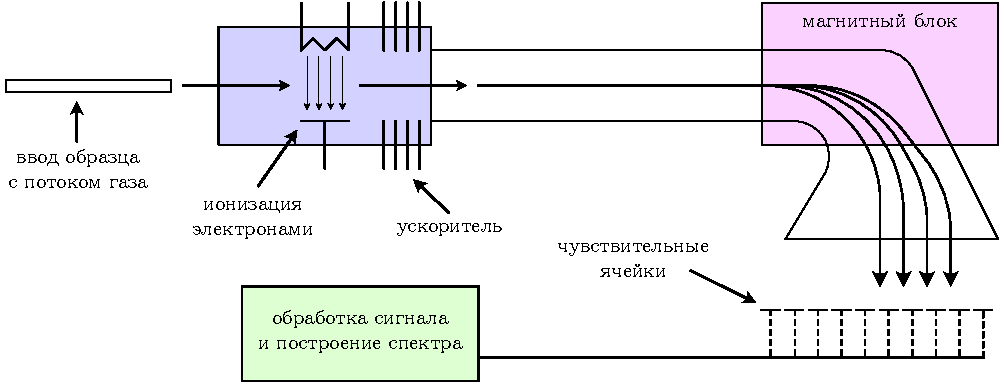
\includegraphics[width=13cm]{figs/definition_of_molar_mass/mass_spectrometer.pdf}
    \caption{Устройство масс-спектрометра.}
    \label{fig:mass_spectrometer}
\end{figure}

Образец вещества превращают в ион путём выбивания из его молекул электронов. При этом может быть выбито один или несколько электронов. Также молекулы вещества могут распадаться с образованием заряженных \emph{фрагментов} исходной молекулы.

Образующиеся ионы ускоряют в электрическом поле а затем они попадают в магнитное поле, в котором разделяются. Радиус кривизны траектории ионов зависит от квадратного корня отношения массы к заряду:

\begin{equation*}
    R \propto \sqrt{\frac{M_r}{z}},
\end{equation*}

где $z$~--- заряд иона.

Ионы попадают на ячейки детектора и после цифровой обработки формируется \emph{спектр}, в котором отдельные пики соответствуют определённым величинам $M_r/z$. Пик с самой большой величиной $M_r/z$ соответствует однократно ионизированной молекуле, которая не претерпела распада. При этом он не обязательно будет самым интенсивным, поскольку молекулярные ионы бывают неустойчивы. Пик с самой большой интенсивностью называют \emph{базовым пиком}, его интенсивность принимают за \qty{100}{\percent}.

Также могут присутствовать так называемые \emph{изотопные пики}, связанные с различным содержанием нуклидов в веществе.

По сути, метод масс-спектрометрии можно считать прямым измерением относительной молекулярной массы.

Также по величине $M_r/z$ осколков молекулы можно сделать вывод о её строении, поскольку связи в молекулах после ионизации разрушаются по определённым правилам.

\subsection*{Метод шприца}

Метод распространён для легкокипящих жидкостей. В основе данного метода лежит уравнение состояния идеального газа:

\begin{equation}
    \label{eq:ideal_gas_law}
    pV = nRT \Longrightarrow M = \frac{mRT}{pV}.
\end{equation}

Используют прибор, изображённый на рис.~\ref{fig:syringe_method}.

\begin{figure}[htbp]
    \centering
    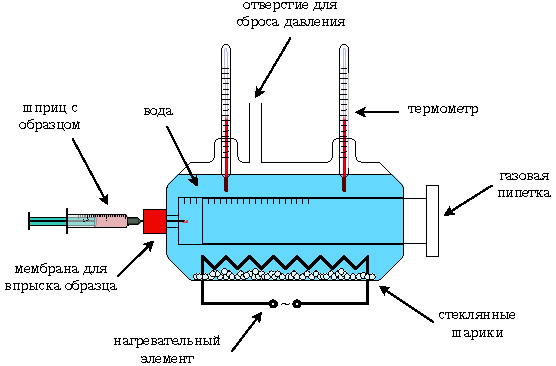
\includegraphics[width=12cm]{figs/definition_of_molar_mass/syringe_method.pdf}
    \caption{Установка для определения молярной массы методом шприца.}
    \label{fig:syringe_method}
\end{figure}

Образец вводят в газовую пипетку, помещённую в рубашку с кипящей дистиллированной водой. По разнице масс шприца до и после введения вещества определяют массу $m$ образца. Вещество испаряется в пипетке и смещает лёгкий поршень до установления равновесия с атмосферным давлением. По разнице положения поршня газовой пипетки до и после ввода определяют объём газа $V$, после чего проводят расчёт молярной массы. Величину атмосферного давления измеряют барометром.

Если есть проблемы с измерением давления, то можно использовать вещество сравнения с известной молярной массой, проведя измерения для него и исследуемого вещества в идентичных условиях. Сократив в выражении~\ref{eq:ideal_gas_law} $RT$ и $p$, получим:

\begin{equation*}
    \frac{M_1}{M_2} = \frac{m_1V_2}{m_2V_1}.
\end{equation*}

\subsection*{Метод Виктора Мейера}

Этот метод также основан на уравнении~\ref{eq:ideal_gas_law} и тоже использует измерение объёма выделившегося при испарении вещества газа, однако имеет несколько другое аппаратурное исполнение (рис.~\ref{fig:Meyer_method}).

\begin{figure}[htbp]
    \centering
    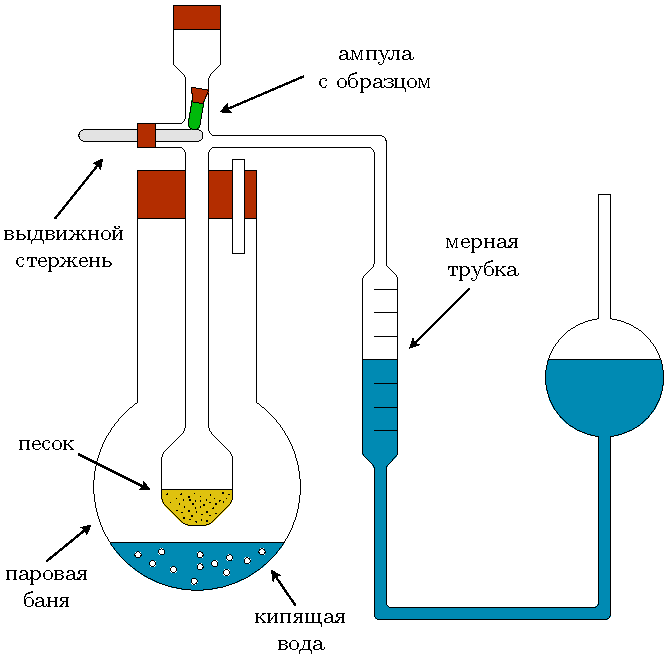
\includegraphics[width=8.5cm]{figs/definition_of_molar_mass/Meyer_method.pdf}
    \caption{Установка для определения молярной массы вещества методом Виктора Мейера.}
    \label{fig:Meyer_method}
\end{figure}

Исследуемый образец помещают в маленькую закрытую ампулу и аккуратно устанавливают внутрь аппарата, как показано на рисунке. Затем нагревают воду в колбе до кипения и сдвигают стержень. Ампула падает на песок, открывается, а содержимое испаряется. При помощи мерной трубки с водяным затвором измеряют объём воздуха, вытесненного паром и далее рассчитывают молярную массу аналогично методу шприца.

\clearpage

\section{Уравнения химических реакций~--- знакомство}

\hspace*{\parindent}Как вы уже знаете, превращение одних веществ в другие называется \hyperref[term:chemical_reaction]{химической реакцией}. При этом не происходит превращения атомов химических элементов друг в друга, а происходит перераспределение химических связей между атомами.

Запись происходящих изменений и называют \textbf{уравнением химической реакции}\label{term:chemical_equation}\index{уравнение реакции}. Давайте учиться записывать и читать такие уравнения.

Общую схему уравнения химической реакции можно представить в следующем (довольно громоздком) виде. \textbf{Чёрным} цветом обозначены обязательные элементы уравнения, а \textcolor{red}{красным} и \textcolor{blue}{синим}~--- необязательные.

\begin{equation*}
    \overbrace{\textcolor{blue}{i}\mathrm{A}_{\text{\textcolor{red}{(состояние)}}} + \textcolor{blue}{j}\mathrm{B}}^{\text{исходные вещества}} \;\;\; \underbrace{\xrightarrow{\text{\textcolor{red}{условия реакции}}}}_{\text{знак разделения}} \;\;\; \overbrace{\textcolor{blue}{k}\mathrm{C} + \textcolor{blue}{l}\mathrm{D}}^{\text{продукты}}\overbrace{\textcolor{red}{\uparrow} + \text{ \small{\textcolor{red}{(термод. эффект)}}}}^{\text{\textcolor{red}{признаки реакции}}}
\end{equation*}

\subsection*{Исходные вещества и продукты}

Исходные вещества (реагенты) и продукты записывают в левой и правой частях уравнения соответственно, разделяя их специальным знаком. Вещества указывают, разделяя их знаком <<$+$>>, например:

\reaction*{CaO + H2O -> Ca(OH)2{.}}

\subsection*{Кэффициенты}

Рядом с формулой вещества могут стоять \textbf{стехиометрические коэффициенты}\label{term:stoichiometric_coefficient}\index{стехиометрический коэффициент} ($\textcolor{blue}{i}$, $\textcolor{blue}{j}$, $\textcolor{blue}{k}$, $\textcolor{blue}{l}$), обычно представляющие собой положительные целые числа, например:

\reaction{
    \label{ce:equation_example}
    Ca(OH)2 + 2HCl -> CaCl2 + 2H2O{.}
}

Если коэффициент отсутствует, то подразумевается, что он равен 1.

Коэффициенты показывают, в каком количественном соотношении по частицам реагируют и образуются вещества в химической реакции. Например, в приведённой выше реакции гидроксид кальция и соляная кислота вступают в реакцию в соотношении 1:2 по молям.

Иногда используют и дробные коэффициенты (например, если показывают термодинамические эффекты реакции или при подборе коэффициентов):

\reaction*{Al + \frac{3}{2}O2 -> Al2O3{.}}

Необходимость коэффициентов в химической реакции является следствием закона сохранения массы: \emph{атомы не возникают из ниоткуда и не пропадают в никуда}, поэтому в левой и правой частях уравнения количества атомов каждого элемента должны быть равны (\ref{eq:law_of_conservation_of_matter_in_chemical_reactions}):

\begin{equation}
    \label{eq:law_of_conservation_of_matter_in_chemical_reactions}
    \sum_{j \in \text{реаг.}}^{}a_{ij}s_j = \sum_{j \in \text{прод.}}^{}a_{ij}s_j, 
\end{equation}

где $a_{ij}$~--- число атомов химического элемента $i$ в молекуле вещества $j$ (т.~е. сколько атомов входит в состав формульной единицы соединения), $s_j$ стехиометрический коэффициент для вещества $j$.

Например, в уравнении~(\ref{ce:equation_example}) в левой части уравнения имеется $2 + 2 = 4$ атома водорода (по два атома из гидроксида кальция и соляной кислоты), а в правой части такое же количество ($2 \cdot 2 = 4$) атомов водорода находится в составе воды.

Иногда запись химической реакции может не содержать коэффициентов, а только формулы веществ (иногда только исходные). В таком случае говорят не об уравнении, а о \textbf{схеме химической реакции}\label{term:reaction_scheme}\index{схема реакции}.

\subsection*{Знак разделения}

Реагенты и продукты в уравнении химической реакции разделяют определённым знаком для того, чтобы выделить исходные вещества и продукты и показать тип химической реакции. Наиболее распространённые знаки указаны в (табл.~\ref{tab:dividing_marks_in_a_chemical_reaction}).

\begin{table}[htbp]
    \small
    \caption{Знаки разделения исходных веществ и продуктов в уравнениях химических реакций.}
    \label{tab:dividing_marks_in_a_chemical_reaction}
    \begin{tabularx}{\textwidth}{
        >{\hsize=0.2\hsize}Z
        >{\hsize=1.8\hsize}Y
        }
        \hline
        \rowcolor{green!5}
        Символ & Назначение \\
        \hline
        \ce{->} & Односторонняя стрелка, ставится в большинстве случаев. \\
        \hline
        $=$ & Знак равенства. Ставится, когда необходимо обратить внимание на то, что реакция стехиометрически уравнена, то есть соблюдается выражение (\ref{eq:law_of_conservation_of_matter_in_chemical_reactions}). В настоящее время считается устаревшим. \\
        \hline
        \ce{<-->} & Реакция может протекать в прямом и обратном направлении.\\
        \hline
        $\nrightarrow$ & Реакция не идёт. \\
        \hline
    \end{tabularx}
\end{table}

Обратите внимание на знак, состоящий из двух стрелок в прямом и обратном направлении: \ce{<-->}. Такие реакции могут протекать как \emph{слева направо}, так и \emph{справа налево}. То есть если отдельно смешать реагенты или продукты, то будет получена одна и та же смесь, содержащая вещества из левой и правой частей уравнения реакции. Например, азот и водород при смешивании под давлением при нагревании превращается в смесь, содержашую азот, водород и продукт их реакции~--- аммиак. Если в те же условия поместить аммиак, то тоже будет получена смесь азота, водорода и аммиака из-за протекающей в обоих направлениях реакции \ce{N2 + 3H2 <--> 2NH3}. 

\subsection*{Состояние вещества}

Иногда необходимо указать, в каком состоянии находится вещество, либо характеристики его раствора. В таких случаях снизу справа к веществу в круглых скобках можно приписать соответствующее обозначение из табл.~\ref{tab:designation_of_the_state_of_matter}.

\begin{table}[htbp]
    \small
    \caption{Обозначение состояния вещества в реакциях.}
    \label{tab:designation_of_the_state_of_matter}
    \centering 
    \begin{tabular}{ll}
        \hline
        \rowcolor{green!5}Сокращение & Расшифровка \\
        \hline
        (т) или (тв) & твёрдое \\
        (ж) & жидкое \\
        (г) & газообразное \\
        \hline
        (aq) & вещество растворено в воде \\
        (безводн.) & безводный \\
        (влажн.) & влажный \\
        (конц.) & концентрированный раствор \\
        (разб.) & разбавленный раствор \\
        (оч. разб.) & очень разбавленный раствор \\
        \hline
        (гор.) & горячий \\
        (кип.) & кипящий \\
        (хол.) & холодный \\
        (комн.) & комнатная температура \\
        \hline
        (дымящ.) & дымящий \\
        (насыщ.) & насыщенный \\
        \hline
    \end{tabular}
\end{table}

Могут быть указаны и другие необходимые характеристики вещества, например, его цвет.

Такие уточнения могут оказаться очень полезны, поскольку часто одни и те же реагенты, взятые в разном состоянии, приводят к различным продуктам реакции. Вот несколько примеров подобных обозначений, уточняющих особенности проведения реакции:

\reaction*{KNO2 + HCl_{(\text{разб.})} -> KCl + HNO2{;}}
\reaction*{3KNO2_{(\text{т})} + 2HCl_{(\text{конц.})} -> 2KCl + KNO3 + 2NO +H2O{;}}
\reaction*{KNO2 + 2HCl_{(\text{конц.})} -> (NO)Cl + KCl + H2O{.}}

\subsection*{Условия реакции}\label{sec:reaction_conditions}\index{условия реакции}

Многие реакции протекают только при определённых условиях, например, повышенной температуре, давлении и т.~д. Необходимые для осуществления реакции условия записывают либо над знаком реакции, либо после записи уравнения реакции, например:

\reaction*{10KClO3 + 12P ->[\text{выше} \qty{250}{\degreeCelsius}] 10KCl + 3P4O10{;}}
\reaction*{KClO3 + H2O ->[\text{электролиз, Pt-анод}] H2 + KClO4{.}}
\reaction*{MgCO3 -> MgO + CO2 (\text{>} \qty{650}{\degreeCelsius}){;}}
\reaction*{MgCO3 + (NH4)2SO4_{(\text{конц.})} -> MgSO4 + 2NH3 + CO2 + H2O (\text{кип.}){.}}

Наиболее распостранённые обозначения условий реакций (хотя и не все) приведены в табл.~\ref{tab:designation_of_reaction_conditions}.

\begin{table}[htbp]
    \small
    \caption{Обозначение условий реакций.}
    \label{tab:designation_of_reaction_conditions}
    \centering 
    \begin{tabular}{cl}
        \hline
        \rowcolor{green!5}Сокращение & Расшифровка \\
        \hline
        $\Delta$ или t & нагрев \\
        $h\nu$ & облучение \\
        $\tau$  & для протекания реакции требуется время \\
        $p$ & избыточное давление \\
        кат. & катализатор \\
        \hline
    \end{tabular}
\end{table}

\subsection*{Признаки реакции}

Также в уравнениях химических реакций очень часто записывают \hyperref[term:signs_of_a_chemical_reaction]{признаки протекания реакций}. Выделение газа или выпадение осадка в реакционной смеси обозначают стрелками вверх $\uparrow$ и вниз $\downarrow$, стоящими рядом с соответствующими веществами:

\reaction*{2FeCl3 + 3Na2S -> 2FeS (v) + S (v) + 6NaCl{;}}
\reaction*{FeCl3 + 3HF_{(\text{ж})} -> FeF3 (v) +3HCl (^) {.}}

Выделение или поглощение теплоты обозначают символами $+Q$ и $-Q$ после уравнения химической реакции либо непосредственно записывают величину теплового эффекта:

\reaction*{Li2CO3 ->[\num{730}-\qty{1270}{\degreeCelsius}] Li2O + CO2 -$Q${;}}
\reaction*{4NH3_{(\text{г})} + 3O2_{(\text{г})} -> 2N2_{(\text{г})} + 6H2O_{(\text{ж})} \text{\qty[retain-explicit-plus]{+1531}{\kJ}}{.}}

\subsection*{Расстановка коэффициентов}\label{sec:setting_the_coefficients}

Чтобы превратить \emph{схему} химической реакции в \emph{уравнение}, необходимо расставить коэффициенты перед веществами так, чтобы выполнялось соотношение \ref{eq:law_of_conservation_of_matter_in_chemical_reactions}, то есть чтобы число атомов каждого элемента было одинаковым в левой и правой частях уравнения.

После того, как коэффициенты будут расставлены, уравнение станет \textbf{сбалансированным}\label{term:stoichiometrically_balanced_equation}\index{сбалансированное уравнение}. Расстановку коэффициентов можно выполнить тремя способами:

\begin{itemize}
    \item методом подбора;
    \item используя представления об \emph{окислительно-восстановительных реакциях} (если это применимо);
    \item решением системы линейных уравнений.
\end{itemize}

Второй и третий способ мы будем изучать позже, а пока давайте посмотрим, как расставить коэффициенты самым простым методом~--- подбора.

\begin{example}{}{ex:chemical_equations1}
    \textit{Расставьте коэффициенты в реакции:}
    \reaction*{Pb(NO3)2 -> PbO + NO2 + O2{.}}
    \textit{Решение.} Принимаем коэффициент перед нитратом свинца за 1. Тогда в правой части уравнения число атомов свинца сбалансировано~--- также 1. Число атомов азота в нитрате свинца равно 2, а в правой части есть только один атом азота, поэтому ставим 2 перед оксидом азота:
    \reaction*{Pb(NO3)2 -> PbO + {\color{red}2}NO2 + O2{.}}
    Проверяем баланс по атомам кислорода: в левой части $3 \cdot 2 = 6$, в правой части $1 + 2 \cdot 2 + 2 = 7$, не сходится. Чтобы увеличить количество кислорода в левой части, ставим коэффициент 2 перед нитратом свинца и повторяем операции: ставим коэффициент 2 перед оксидом свинца чтобы уравнять количество атомов свинца, 4 перед оксидом азота, чтобы уравнять атомы азота:
    \reaction*{{\color{red}2}Pb(NO3)2 -> {\color{red}2}PbO + {\color{red}4}NO2 + O2{.}}
    Считаем число атомов кислорода. В левой части теперь $2 \cdot 3 \cdot 2 = 12$, в правой части $2 + 4 \cdot 2 + 2 = 12$, сходится. Коэффициенты расставлены верно.
\end{example}

\begin{example}{}{ex:chemical_equations2}
    \textit{Расставьте коэффициенты в реакции:}
    \reaction*{LiH + SO2 -> Li2SO4 + H2S{.}}
    \textit{Решение.} В левой части по одному атому лития и серы, а в правой~--- по два, поэтому ставим Коэффициенты 2 перед исходными веществами:
    \reaction*{{\color{red}2}LiH + {\color{red}2}SO2 -> Li2SO4 + H2S{.}}
    Проверяем баланс по атомам кислорода и водорода. Кислорода по четыре атома слева и справа, водорода по два, баланс сходится, коэффициенты расставлены верно.
\end{example}

\begin{example}{}{ex:chemical_equations3}
    \textit{Расставьте коэффициенты в реакции:}
    \reaction*{PCl5 + P4O10 -> PCl3O{.}}
    \textit{Решение.} Слева пять атомов фосфора, а справа~--- один, поэтому ставим 5 перед оксидом-трихлоридом фосфора:
    \reaction*{PCl5 + P4O10 -> {\color{red}5}PCl3O{.}}
    Теперь оказалось, что слева 10 атомов кислорода, а справа~--- 5. Поэтому удваиваем коэффициент перед оксидом-трихлоридом фосфора:
    \reaction*{PCl5 + P4O10 -> {\color{red}10}PCl3O{.}}
    Теперь оказалось, что справа 10 атомов фосфора, а слева~--- 5. Добавляем коэффициент 6 перед хлоридом фосфора:
    \reaction*{{\color{red}6}PCl5 + P4O10 -> 10PCl3O{.}}
    Проверяем баланс по атомам хлора: слева $6 \cdot 5 = 30$ атомов, справа $10 \cdot 3 = 30$ атомов. Баланс сходится по всем элементам, уравнение сбалансировано.
\end{example}

\begin{example}{}{ex:chemical_equations4}
    \textit{Расставьте коэффициенты в реакции:}
    \reaction*{Na3PO4 + Ca(NO3)2 -> Ca3(PO4)2 (v) + NaNO3{.}}
    \textit{Решение.} При расстановке коэффициентов можно оперировать не только отдельными атомами, но и \emph{устойчивыми группами} атомов, которые перемещаются в ходе реакции без изменений. Если вы внимательно изучите данную реакцию, то заметите, что в ней группы \ce{PO4}, \ce{NO3}, \ce{Na} и \ce{Ca} просто перемещаются между веществами без изменения, поэтому их можно считать одним целым при подсчёте. Справа три атома кальция, а слева только один, поэтому ставим коэффициент 3 перед нитратом кальция:
    \reaction*{Na3PO4 + {\color{red}3}Ca(NO3)2 -> Ca3(PO4)2 (v) + NaNO3{.}}
    Теперь слева стало шесть нитратных групп \ce{NO3} и нужно поставить коэффициент 6 перед нитратом натрия:
    \reaction*{Na3PO4 + 3Ca(NO3)2 -> Ca3(PO4)2 (v) + {\color{red}6}NaNO3{.}}
    Теперь, чтобы уравнять атомы натрия, необходимо поставить коэффициент 2 перед фосфатом натрия:
    \reaction*{{\color{red}2}Na3PO4 + 3Ca(NO3)2 -> Ca3(PO4)2 (v) + 6NaNO3{.}}
    Теперь количество всех групп в уравнении сбалансировано.
\end{example}

Давайте повторим полученные знания и перейдём к решению задач.

\begin{termlist}
    \hyperref[term:chemical_equation]{Уравнение реакции}, 
    \hyperref[term:stoichiometric_coefficient]{стехиометрический коэффициент},
    \hyperref[term:reaction_scheme]{схема реакции},
    \hyperref[sec:reaction_conditions]{условия реакции},
    \hyperref[term:stoichiometrically_balanced_equation]{сбалансированное уравнение}.
\end{termlist}

\begin{problem}{}{chemical_equations1}
    Подберите коэффициенты для следующих реакций:
    \begin{enumerate}[label=\arabic*)]
        \item \ce{H2 + O2 -> H2O{;}}
        \item \ce{Na + H2O -> NaOH + H2{;}}
        \item \ce{P + O2 -> P2O5{;}}
        \item \ce{H2 + N2 -> NH3{.}}
    \end{enumerate}
    \begin{sol}{\ref{prob:chemical_equations1}}
        \begin{enumerate}[label=\arabic*)]
            \item \ce{2H2 + O2 -> 2H2O{;}}
            \item \ce{2Na + 2H2O -> 2NaOH + H2{;}}
            \item \ce{2P + 5O2 -> 2P2O5{;}}
            \item \ce{3H2 + N2 -> 2NH3{.}}
        \end{enumerate}
    \end{sol}
\end{problem}

\begin{problem}{}{chemical_equations2}
    Подберите коэффициенты для следующих реакций:
    \begin{enumerate}[label=\arabic*)]
        \item \ce{H2SO4 + Ca(OH)2 -> CaSO4 + H2O{;}}
        \item \ce{Ba(OH)2 + H2SO4 -> BaSO4 (v) + H2O{;}}
        \item \ce{K2CO3 + 2HCl -> 2KCl + CO2 (^) + H2O{;}}
        \item \ce{NO2 + Cu ->[\qty{600}{\degreeCelsius}] N2 + CuO{.}}
    \end{enumerate}
    \begin{sol}{\ref{prob:chemical_equations2}}
        \begin{enumerate}[label=\arabic*)]
            \item \ce{H2SO4 + Ca(OH)2 -> CaSO4 + 2H2O{;}}
            \item \ce{Ba(OH)2 + H2SO4 -> BaSO4 (v) + 2H2O{;}}
            \item \ce{K2CO3 + 2HCl -> 2KCl + CO2 (^) + H2O{;}}
            \item \ce{2NO2 + 4Cu ->[\qty{600}{\degreeCelsius}] N2 + 4CuO{.}}
        \end{enumerate}
    \end{sol}
\end{problem}

\begin{problem}{}{chemical_equations3}
    Подберите коэффициенты для следующих реакций:
    \begin{enumerate}[label=\arabic*)]
        \item \ce{WCl6 ->[$> \qty{350}{\degreeCelsius}$] WCl5 + Cl2{;}}
        \item \ce{PBr5 + H2O -> H3PO4 + HBr{;}}
        \item \ce{NaClO2 + HCl_{(\text{конц.})} -> Cl2 (^) + NaCl + H2O{;}}
        \item \ce{Li2C2 + SO2 -> Li2O + CO + S{.}}
    \end{enumerate}
    \begin{sol}{\ref{prob:chemical_equations3}}
        \begin{enumerate}[label=\arabic*)]
            \item \ce{2WCl6 ->[$> \qty{350}{\degreeCelsius}$] 2WCl5 + Cl2{;}}
            \item \ce{PBr5 + 4H2O -> H3PO4 + 5HBr{;}}
            \item \ce{NaClO2 + 4HCl_{(\text{конц.})} -> 2Cl2 (^) + NaCl + 2H2O{;}}
            \item \ce{2Li2C2 + 3SO2 -> 2Li2O + 4CO + 3S{.}}
        \end{enumerate}
    \end{sol}
\end{problem}

\clearpage

\section{Расчёты по химическим уравнениям}\label{sec:calculations_based_on_chemical_equations}

\hspace*{\parindent}Имея сбалансированное уравнение химической реакции с \hyperref[sec:setting_the_coefficients]{правильно} расставленными коэффициентами, мы можем, используя \hyperref[term:stoichiometric_relations]{основные стехиометрические соотношения}, рассчитать количества реагентов и продуктов до, во время и после реакции. При этом нам должна быть известна информация о количестве хотя бы одного из участвующих в реакции веществ.

Вещества реагируют друг с другом в определённом соотношении, определяемом коэффициентами в уравнении реакции. Коэффициенты показывают пропорции веществ \emph{по числу реагирующих частиц}. Например, при горении железа в хлоре

\reaction*{2Fe + 3Cl2 -> 2FeCl3}

два атома железа вступают в реакцию с тремя молекулами хлора и образуются две молекулы \ce{FeCl3}. Или, другими словами, на 2 моль железа потребуется 3 моль хлора, чтобы железо полностью прореагировало.

Математически мы можем записать выражение для связи количеств веществ, участвующих в \emph{одной реакции} таким образом:

\begin{equation}
    \frac{n_i}{s_i} = \text{const}, 
\end{equation}

где $n_i$~---количество $i$-го вещества в реакции, $s_i$~--- коэффициент перед этим веществом в уравнении реакции.

Чтобы перейти к массам веществ, запишем количество вещества $n_i$ через массу и молярную массу:

\begin{equation}
    \label{eq:balance_by_quantity_of_substances}
    \fbox{$\displaystyle\frac{m_i}{s_iM_i} = \text{const}$}. 
\end{equation}

Например, для уравнения реакции

\reaction*{2NaOH + H3PO4 -> Na2HPO4 + 2H2O}

выражение~(\ref{eq:balance_by_quantity_of_substances}) будет иметь вид:

\begin{equation*}
    \frac{m(\ce{NaOH})}{2M(\ce{NaOH})} = \frac{m(\ce{H3PO4})}{M(\ce{H3PO4})} = \frac{m(\ce{Na2HPO4})}{M(\ce{Na2HPO4})} = \frac{m(\ce{H2O})}{2M(\ce{H2O})}.
\end{equation*}

Количественные расчёты по уравнениям реакций в основном и строятся с использованием выражения~(\ref{eq:balance_by_quantity_of_substances}).

\begin{example}{}{ex:calculations_based_on_chemical_equations1}
    \textit{В реакции}
    \reaction*{Na2S + 2O2 ->[\Delta] Na2SO4}
    \textit{было израсходовано 5~г кислорода. Сколько продукта реакции образовалось?}

    \medskip
    \textit{Решение.} Составляем выражение (\ref{eq:balance_by_quantity_of_substances}) для интересующих нас веществ и выражаем массу сульфата натрия:
    \begin{equation*}
        \frac{m(\ce{O2})}{2M(\ce{O2})} = \frac{m(\ce{Na2SO4})}{M(\ce{Na2SO4})} \Longrightarrow m(\ce{Na2SO4}) = \frac{m(\ce{O2})M(\ce{Na2SO4})}{2M(\ce{O2})}.
    \end{equation*}
    $M(\ce{O2}) = 2 \cdot \num{15,999} = \qty{31,998}{\g\per\mole}$, \\$M(\ce{Na2SO4}) = 2 \cdot \num{22,99} + \num{32,06} + 4 \cdot \num{15,999} = \qty{142.036}{\g\per\mole}$.
    \begin{equation*}
        m(\ce{Na2SO4}) = \frac{5 \cdot \num{142,036}}{2 \cdot \num{31,998}} = \qty{11,097}{\g}.
    \end{equation*}
\end{example}

Выражение (\ref{eq:balance_by_quantity_of_substances}) можно переписать и с использованием других выражений для количества вещества, например, через объёмы (если в реакцию вступают газы) или число частиц.

При этом молярный объём и число Авогадро можно внести в константу, но только если мы используем объёмы или число частиц для всех веществ в расчёте. Например, если при расчёте используются и массы веществ, и объёмы газов, вносить молярный объём в константу нельзя. 

\begin{equation}
    \label{eq:balance_by_volume_of_substances}
    \frac{V_i}{s_iV_m} = \text{const} \rightsquigarrow \frac{V_i}{s_i} = \text{const'}, 
\end{equation}
\begin{equation}
    \frac{N_i}{s_iN_A} = \text{const} \rightsquigarrow \frac{N_i}{s_i} = \text{const'}. 
\end{equation}

\begin{example}{}{ex:calculations_based_on_chemical_equations2}
    \textit{В реакции синтеза аммиака образовалось \qty{250}{\l} продукта:}
    \reaction*{3H2 + N2 -> 2NH3{.}}
    \textit{Какие объёмы водорода и азота были взяты для синтеза, если их объём измерялся при тех же условиях (температура, даление).}

    \medskip
    \textit{Решение.} Согласно выражению (\ref{eq:balance_by_volume_of_substances}) объёмы водорода и азота будут равны
    \begin{equation*}
        \frac{V(\ce{H2})}{3} = V(\ce{N2}) = \frac{V(\ce{NH3})}{2}.
    \end{equation*}
    \begin{equation*}
        V(\ce{H2}) = \frac{3V(\ce{NH3})}{2} = \frac{3 \cdot 250}{2} = \qty{375}{\l}.
    \end{equation*}
    \begin{equation*}
        V(\ce{N2}) = \frac{V(\ce{NH3})}{2} = \frac{250}{2} = \qty{125}{\l}.
    \end{equation*}
\end{example}

\subsection*{Избыток и недостаток реагентов}

Соотношение реагентов, при котором они без остатка реагируют друг с другом, называется \textbf{стехиометрическим соотношением}\label{term:stoichiometric_ratio}\index{стехиометрическое соотношение}.

В реально протекающих реакциях стехиометрическое соотношение веществ соблюдается редко. Обычно одного из них оказывается больше, чем нужно для того, чтобы полностью прореагировало другое вещество, участвующее в реакции. Если так происходит, то говорят, что вещество находится \textbf{в избытке}\label{term:excess_of_reagent}\index{избыток реагента}.

То вещество, которое должно прореагировать полностью, находится \textbf{в недостатке}\label{term:limiting_reagent}\index{недостаток реагента}.

\begin{example}{}{ex:calculations_based_on_chemical_equations3}
    \textit{В каком стехиометрическом соотношении (по массе) нужно смешать красный фосфор с иодом, чтобы оба вещества полностью прореагировали друг с другом согласно реакции:}
    \reaction*{2P + 3I2 -> 2PI3 (\text{комн., в } CS2){?}}

    \medskip
    \textit{Решение.} Воспользовавшись формулой (\ref{eq:balance_by_quantity_of_substances}) выразим соотношение масс веществ, которые должны быть взяты для реакции.
    \begin{equation*}
        \frac{m(\ce{P})}{2M(\ce{P})} = \frac{m(\ce{I2})}{3M(\ce{I2})},
    \end{equation*}
    \begin{equation*}
        \frac{m(\ce{P})}{m(\ce{I2})} = \frac{2M(\ce{P})}{3M(\ce{I2})} = \frac{2 \cdot \num{30,974}}{3 \cdot (2 \cdot \num{126,9})} = \frac{\num{61,948}}{\num{761,4}} = \frac{1}{\num{12,29}}.
    \end{equation*}
\end{example}

\begin{example}{}{ex:calculations_based_on_chemical_equations4}
    \textit{Смешали по \qty{10}{\g} порошка железа и серы, затем смесь нагрели:
    \reaction*{Fe + S ->[\Delta] FeS{.}}
    Какое вещество осталось непрореагировавшим после окончания реакции и в каком количестве?}

    \medskip
    \textit{Решение.} Сначала определим, какое вещество было в недостатке. Для этого сравним соотношения ${m}/{sM}$. Для железа:
    \begin{equation*}
        \frac{m(\ce{Fe})}{M(\ce{Fe})} = \frac{10}{\num{55,845}} = \num{0,179}.
    \end{equation*}
    Для серы:
    \begin{equation*}
        \frac{m(\ce{S})}{M(\ce{S})} = \frac{10}{\num{32,06}} = \num{0,312}.
    \end{equation*}
    Следовательно, железо было в недостатке в реакционной смеси. Рассчитываем, сколько прореагировало серы:
    \begin{equation*}
        m(\ce{S}) = \frac{m(\ce{Fe})M(\ce{S})}{M(\ce{Fe})} = \frac{10 \cdot \num{32,06}}{\num{55,845}} = \qty{5,741}{\g}.
    \end{equation*}
    Оставшееся количество серы равно $10 - \num{5,741} = \qty{4,259}{\g}$.
\end{example}

Повторите изученные в этом разделе термины, а затем переходите к решению задач.

\begin{termlist}
    \hyperref[term:stoichiometric_ratio]{Стехиометрическое соотношение}, 
    \hyperref[term:excess_of_reagent]{избыток реагента},
    \hyperref[term:limiting_reagent]{недостаток реагента}.
\end{termlist}

\begin{problem}{}{calculations_based_on_chemical_equations1}
    Какую навеску оксида меди (II) необходимо взять, чтобы получить \qty{5}{\g} меди при проведении реакции
    \reaction*{CuO + H2 ->[\Delta] Cu + H2O{?}}
    \begin{sol}{\ref{prob:calculations_based_on_chemical_equations1}}
        Воспользовавшись соотношением~(\ref{eq:balance_by_quantity_of_substances}), находим:
        \begin{equation*}
            \frac{m(\ce{CuO})}{M(\ce{CuO})} = \frac{m(\ce{Cu})}{M(\ce{Cu})} \Longrightarrow m(\ce{CuO}) = \frac{m(\ce{Cu})M(\ce{CuO})}{M(\ce{Cu})} = \frac{5 \cdot \num{79,545}}{\num{63,546}} = \qty{6,259}{\g}.
        \end{equation*}
    \end{sol}
\end{problem}

\begin{problem}{}{calculations_based_on_chemical_equations2}
    Смешали \qty{250}{\l} водорода и \qty{200}{\l} кислорода. Какой газ оказался в избытке и сколько его останется после проведения реакции
    \reaction*{2H2 + O2 -> 2H2O{?}}
    \begin{sol}{\ref{prob:calculations_based_on_chemical_equations2}}
        Объёмы газов при одинаковых условиях пропорциональны количеству вещества, поэтому согласно уравнению реакции стехиометрическим соотношением водорода и кислорода является 2:1. На \qty{250}{\l} водорода требуется \qty{125}{\l} кислорода, а у нас его \qty{200}{\l}, следовательно, \emph{кислород находится в избытке} и после проведения реакции его останется $200 - 125 = \qty{75}{\l}$.
    \end{sol}
\end{problem}

\begin{problem}{}{calculations_based_on_chemical_equations3}
    Расставьте коэффициенты в уравнении реакции и вычислите, сколько кубических метров кислорода (при н.~у.) необходимо взять для сжигания \qty{5}{\kg} метана?    \reaction*{CH4 + O2 -> CO2 + H2O{.}}
    \begin{sol}{\ref{prob:calculations_based_on_chemical_equations3}}
        В правой части уравнения три атома кислорода, а в левой~--- два. Поэтому ставим коэффициент 2 перед водой и 2 перед кислородом. Теперь баланс по атомам водорода и углерода сходится.
        \reaction*{CH4 + 2O2 -> CO2 + 2H2O{.}}
        Масса метана и объём кислорода связаны соотношением:
        \begin{equation*}
            \frac{m(\ce{CH4})}{M(\ce{CH4})} = \frac{V(\ce{O2})}{2V_m}.
        \end{equation*} 
        Поскольку масса выражена в килограммах, а объём~--- в кубических метрах, используем молярную массу в \unit{\kg\per\kmole}, а молярный объём~--- в $\unit{\kl\per\kmole} = \unit{\m^3\per\kmole}$:
        \begin{equation*}
            V(\ce{O2}) = \frac{2m(\ce{CH4})V_m}{M(\ce{CH4})} = \frac{2 \cdot 5 \cdot \num{22,4}}{\num{16,043}} = \qty{13,96}{\m^3}.
        \end{equation*}
        \begin{equation*}
            [V(\ce{O2})] = \frac{\unit{\cancel\kg} \cdot \unit{\m^3} \cdot \unit{\cancel\kmole}}{\unit{\cancel\kg} \cdot \unit{\cancel\kmole}} = \unit{\m^3}.
        \end{equation*}
    \end{sol}
\end{problem}

\begin{problem}{}{calculations_based_on_chemical_equations4}
    $\bigstar$ \qty{5}{\g} неизвестного металла ввели в реакцию с соляной кислотой. При этом выделилось \qty{1,713}{\l} водорода. Что это был за металл?
    \begin{sol}{\ref{prob:calculations_based_on_chemical_equations4}}
        Нам неизвестны коэффициенты в уравнении реакции металла с соляной кислотой чтобы составить стехиометрическое соотношение металла и водорода, поэтому рассмотрим возможные случаи. Обозначим за $x$ количество вещества металла, которое требуется для образования 1~моль молекул $\ce{H2}$. Если металл после реакции образовал хлорид проявляя валентность (I), то значит требовалось 2~моль металла, чтобы образовать 1~моль $\ce{H2}$:
        \begin{equation*}
            2\overset{\text{I}}{\ce{Me}} \leadsto \ce{H2}.
        \end{equation*}
        Если металл проявил валентность (II), то его было нужно 1~моль:
        \begin{equation*}
            \overset{\text{II}}{\ce{Me}} \leadsto \ce{H2}.
        \end{equation*}
        Если металл проявил валентность (III), то его было нужно $2/3$~моль:
        \begin{equation*}
            \frac{2}{3}\overset{\text{III}}{\ce{Me}} \leadsto \ce{H2}.
        \end{equation*}
        Если валентность (IV), то 1/2~моль:
        \begin{equation*}
            \frac{1}{2}\overset{\text{IV}}{\ce{Me}} \leadsto \ce{H2}.
        \end{equation*}
        Б\'{о}льшие валентности маловероятны. Тогда:
        \begin{equation*}
            \frac{m(\ce{Me})}{xM(\ce{Me})} = \frac{V(\ce{H2})}{V_m}.
        \end{equation*}
        Отсюда рассчитываем $xM(\ce{Me})$:
        \begin{equation*}
            xM(\ce{Me}) = \frac{m(\ce{Me})V_m}{V(\ce{H2})} = \frac{5 \cdot 22,4}{\num{1,713}} = \qty{65,38}{\g\per\mole}.
        \end{equation*}
        Далее рассчитываем возможные молярные массы металла, сравнивая их со стандартными атомными весами в \hyperref[appendix:periodic_table]{периодической таблице}. При этом обращаем внимание на группу, в которой находится элемент (оцениваем, может ли он проявлять валентность, которую мы предполагаем).\\
        Если $x = 2$ (валентность (I)), то $M = \qty{32,69}{\g\per\mole}$, таких металлов нет.\\
        Если $x = 1$ (валентность (II)), то $M = \qty{65,38}{\g\per\mole}$~--- \emph{это цинк} (группа в периодической таблице и масса совпадают)!\\
        Если $x = 2/3$ (валентность (III)), то $M = \qty{98,07}{\g\per\mole}$, таких металлов нет.\\
        Если $x = 1/2$ (валентность (IV)), то $M = \qty{130,76}{\g\per\mole}$, таких металлов нет.\\
        Вывод: неизвестный металл~--- цинк.
    \end{sol}
\end{problem}

\clearpage

\section{Выход химической реакции}

\hspace*{\parindent}Теперь вы умеете \hyperref[sec:calculations_based_on_chemical_equations]{рассчитывать количество веществ}, которые образуются в химической реакции.

Масса вещества-продукта, рассчитанная из массы какого-нибудь из исходных веществ по уравнению реакции, называется \textbf{теоретическим выходом}\label{term:theoretical_yield}\index{теоретический выход реакции} и обозначается $m_{\text{теор.}}$. Разумеется, рассчитывать его необходимо по такому исходному веществу, которое было в недостатке в реакционной смеси, потому что именно оно определяет массу образующихся продуктов.

Однако на практике в лаборатории или на промышленном предприятии масса получаемого продукта всегда оказывается меньше, чем рассчитанная. Теоретический выход не может быть достигнут никогда, и вот три основные причины этого:

\begin{itemize}
    \item часть продукта остаётся в реакционной массе или теряется в ходе его сбора, например, остаётся на стенках сосудов, реакторов, испаряется в случае жидких веществ и т.~п. То есть происходят \emph{потери продукта} при его выделении;
    \item исходное вещество не всегда реагирует полностью, часть может остаться непрореагировавшей, особенно в случае равновесных реакций. В этом случае говорят о \emph{низкой конверсии} исходных веществ;
    \item реакция не всегда идёт по одному пути, часто одновременно протекает несколько \emph{конкурирующих реакций}, которые приводят к образованию и других веществ в дополнение к основным продуктам реакции. Если большое количество реагентов расходуется в конкурирующих реакциях, то говорят о \emph{низкой селективности} реакции.
\end{itemize}

Масса продукта, который получен в реальных условиях синтеза, называется \textbf{практическим выходом}\label{term:actual_yield}\index{практический выход реакции} $m_{\text{практ.}}$.

Так как теоретический выход недостижим, людям приходится мириться с потерями и стараться сократить их до минимума, что является одной из задач работы химиков-технологов\footnote{Химик-технолог, в отличие от химика-исследователя~--- это инженер, который сочетает в себе хорошие знания химии со знаниями принципов работы и расчёта технологического оборудования, а также экономики производства. Именно химик-технолог способен масштабировать химическую реакцию <<в колбе>> до промышленного синтеза.}. Особенно это важно в промышленности, где низкий практический выход реакции означает прямую потерю денег.

В синтетической лаборатории, где зачастую цель~--- именно показать возможность синтеза вещества в заданных условиях, количество реально получаемого продукта может играть не главную роль.

Чтобы оценить количество полученного продукта относительно теоретически возможного, используют \textbf{выход химической реакции}\label{term:yield}\index{выход химической реакции} $\eta$. Он вычисляется в процентах и равен отношению полученной на практике массы продукта к теоретическому выходу:

\begin{equation}
    \label{eq:yield}
    \fbox{$\displaystyle\eta = \frac{m_{\text{практ.}}}{m_{\text{теор.}}} \cdot \qty{100}{\percent}$}.
\end{equation}

Для расчёта выхода реакции, разумеется, можно использовать не только массы, но и количества веществ, а для газов~--- также их объёмы:

\begin{equation*}
    \eta = \frac{n_{\text{практ.}}}{n_{\text{теор.}}} \cdot \qty{100}{\percent} = \frac{V_{\text{практ.}}}{V_{\text{теор.}}} \cdot \qty{100}{\percent}.
\end{equation*}

\begin{example}{}{ex:yield1}
    \textit{Химик взял навеску карбоната кальция массой \qty{25}{\g} и прокалил:}
    \reaction*{CaCO3 ->[\Delta] CaO + CO2 (^) {.}}
    \textit{После остывания он собрал образовавшийся оксид кальция и взвесил его. Масса продукта оказалась равна \qty{12}{\g}. Каков оказался выход реакции?}

    \medskip
    \textit{Решение.} Вначале рассчитаем теоретический выход:
    \begin{equation*}
        m_{\text{теор.}}(\ce{CaO}) = \frac{m(\ce{CaCO3})M(\ce{CaO})}{M(\ce{CaCO3})} = \frac{25 \cdot \num{56,077}}{\num{100,086}} = \qty{14,007}{\g}.
    \end{equation*}
    Тогда выход реакции согласно выражению (\ref{eq:yield}) будет равен:
    \begin{equation*}
        \eta = \frac{m_{\text{практ.}}(\ce{CaO})}{m_{\text{теор.}}(\ce{CaO})} \cdot \qty{100}{\percent} = \frac{12}{\num{14,007}} \cdot \qty{100}{\percent} = \qty{85,67}{\percent}.
    \end{equation*}
\end{example}

\subsection*{Арифметический демон и борьба с ним}

Насколько хороший выход реакции является залогом успеха для химиков, почему он так важен? Разве есть большая разница, скажем, между выходом в \qty{90}{\percent} и \qty{95}{\percent}?

Всё дело в том, что обычно редко бывает так, что коммерчески производимые вещества изготавливаются в одну стадию (то есть в результате проведения одной реакции). Обычно осуществляется цепочка реакций из простых веществ-предшественников, так называемых \emph{строительных блоков}, которые доступны для покупки на рынке химических веществ и имеют сравнительно невысокую стоимость. В ходе проведения цепочки реакций продукт каждой из них становится исходным веществом для следующей реакции и так далее. Промежуточные вещества в цепочке синтеза называются \emph{полупродуктами синтеза}. Полупродукты постепенно усложняются, пока, наконец, не станут необходимым продуктом производства или лабораторного синтеза:

\reaction*{A1 ->[$\eta_1$] A2 ->[$\eta_2$] A3 -> $\ldots$ -> A10 ->[$\eta_{10}$] \text{продукт}{.}}

Также обычно после выделения продукта происходят стадии \emph{очистки}, сопровождающиеся частичной потерей продукта. Эти стадии с собственным выходом тоже можно включить в схему получения вещества. Такие длинные производственные цепочки особенно характерны для синтеза органических веществ.

Подобная последовательность получения вещества называется \textbf{линейной схемой синтеза}\label{term:linear_synthetic_pathway}\index{линейная схема синтеза}.

Представим, что выход на каждой стадии составляет 60 или \qty{90}{\percent}. Тогда итоговый выход цепочки синтеза будет равен произведению выходов отдельных стадий:

\begin{equation*}
    \eta_{\qty{60}{\percent}} = \num{0,6}^{10} \cdot \qty{100}{\percent} = \qty{0,6}{\percent},
\end{equation*}
\begin{equation*}
    \eta_{\qty{90}{\percent}} = \num{0,9}^{10} \cdot \qty{100}{\percent} = \qty{34,9}{\percent},
\end{equation*}

Видите, как быстро практический выход цепочки реакций превращается в ничто при снижении выходов отдельных стадий? Такое поведение называется \textbf{арифметическим демоном}\label{term:multiplicative_yield_loss_in_linear_syntheses}\index{арифметический демон}\footnote{В англоязычной литературе термин <<арифметический демон>> не используется, а применяется скучное выражение <<\textit{multiplicative yield loss in linear syntheses}>>~--- проблема мультипликативных потерь выхода в линейных синтезах.}. Разница между \qty{0,6}{\percent} и \qty{34,9}{\percent} общего выхода означает, что при повышении выхода на каждой стадии с 60 до \qty{90}{\percent} вы получаете в 58 раз больше конечного продукта ($\frac{\num{34,9}}{\num{0,6}} \approx \num{58,2}$). Поэтому даже небольшое повышение выхода на отдельных стадиях критически важно для эффективности многостадийного синтеза.

Как нам бороться с этим явлением? Допустим, мы вместо постепенного усложнения соединения от стадии к стадии синтезируем два сложных предшественника \ce{A6} и \ce{B5}, из которых на последней стадии получим необходимое вещество:

\reaction*{A1 -> A2 -> $\ldots$ -> A6 (\text{пять стадий}){,}}
\reaction*{B1 -> B2 -> $\ldots$ -> B5 (\text{четыре стадии}){,}}
\reaction*{A6 + B5 -> \text{продукт}{,} (\text{одна стадия}){.}}

Итого в этой цепочке тоже 10 стадий, но выход составит уже

\begin{equation*}
    \eta_{\qty{60}{\percent}} = \num{0,6}^6 \cdot \qty{100}{\percent} = \qty{4,7}{\percent},
\end{equation*}
\begin{equation*}
    \eta_{\qty{90}{\percent}} = \num{0,9}^6 \cdot \qty{100}{\percent} = \qty{53,1}{\percent}.
\end{equation*}

Такие схемы синтеза называются \textbf{конвергентными}\label{term:convergent_synthesis_scheme}\index{конвергентная схема синтеза}, и они всегда более предпочтительны при прочих равных условиях. Кроме преимущества в выходе продукта они также позволяют экономить время, параллельно синтезируя вещества-предшественники.

Теперь давайте повторим изученные понятия и решим пару задач ниже.

\begin{termlist}
    \hyperref[term:theoretical_yield]{Выход реакции}, 
    \hyperref[term:actual_yield]{практический выход реакции},
    \hyperref[term:yield]{выход химической реакции},
    \hyperref[term:linear_synthetic_pathway]{линейная схема синтеза},
    \hyperref[term:multiplicative_yield_loss_in_linear_syntheses]{арифметический демон},
    \hyperref[term:convergent_synthesis_scheme]{конвергентная схема синтеза}.
\end{termlist}

\begin{problem}{}{yield1}
    \qty{11,495}{\g} металлического натрия прореагировало с избытком воды, при этом удалось собрать \qty{4,48}{\l} водорода (н.~у.):
    \reaction*{2Na + 2H2O -> 2NaOH + H2 (^) {.}}
    Рассчитайте выход реакции.
    \begin{sol}{\ref{prob:yield1}}
        Рассчитаем теоретический выход водорода в молях. Количество вещества образовавшегося водорода вдвое меньше, чем израсходованного натрия, т.~е.
        \begin{equation*}
            n(\ce{H2})_{\text{теор.}} = \frac{n(\ce{Na})}{2} = \frac{m(\ce{Na})}{2M(\ce{Na})} = \frac{\num{11,495}}{2 \cdot \num{22,99}} = \qty{0,25}{\mole}.
        \end{equation*}
        Количество вещества собранного водорода равно:
        \begin{equation*}
            n(\ce{H2})_{\text{практ.}} = \frac{V_{\text{практ.}}(\ce{H2})}{V_m} = \frac{\num{4,48}}{22,4} = \qty{0,2}{\mole}.
        \end{equation*}
        Наконец, рассчитываем выход реакции:
        \begin{equation*}
            \eta = \frac{n_{\text{практ.}}}{n_{\text{теор.}}} \cdot \qty{100}{\percent} = \frac{\num{0,2}}{\num{0,25}} \cdot \qty{100}{\percent} = \qty{80}{\percent}.
        \end{equation*}
    \end{sol}
\end{problem}

\begin{problem}{}{yield2}
    При синтезе некоторого химического соединения используется 5 химических реакций. Напишите максимально линейную и максимально конвергентную возможные схемы синтеза этого продукта.
    \begin{sol}{\ref{prob:yield2}}
        Максимально линейная схема:
        \reaction*{A1 -> A2 -> A3 -> A4 -> A5 -> \text{продукт}{.}}
        Максимально конвергентная схема синтеза будет такой:
        \reaction*{A1 -> B1{;}}
        \reaction*{A2 -> B2{;}}
        \reaction*{A3 -> B3{;}}
        \reaction*{A4 -> B4{;}}
        \reaction*{B1 + B2 + B3 + B4 -> \text{продукт}{.}}
    \end{sol}
\end{problem}

\begin{problem}{}{yield3}
    $\bigstar$ Вы как раз читали раздел, посвящённый выходу химической реакции, когда в аудиторию ворвался невероятно возбуждённый и помятый \textit{профессор Недоумелкин}. <<Сенсация! Скоро обо мне узнает весь мир!>> --- кричит он. Когда вы его немного успокоили и расспросили, в чём дело, он рассказал, что работал в лаборатории и после того, как взвесил полученный продукт реакции, оказалось, что выход составил больше \qty{100}{\percent}. <<Законы природы нельзя обмануть>>, --- сказали вы ему и объяснили, почему так могло получиться. Что вы ему сказали?
    \begin{sol}{\ref{prob:yield3}}
        Причинами кажущегося выхода более \qty{100}{\percent} могли быть некоторые из следующих вариантов:
        \begin{itemize}
            \item в выделенный продукт попали примеси, которые увеличили его массу. Это мог быть не до конца испаренный растворитель, непрореагировавший реагент, побочные продукты реакции, адсорбированные газы, загрязнения от посуды и пр.;
            \item была неправильно оценена чистота исходных веществ, и в них были примеси, которые могли давать тот же продукт. Например, карбонат кальция \ce{CaCO3} часто содержит карбонат магния \ce{MgCO3}. При разложении оба образуют \ce{CO2}, но расчёт мог вестись только по содержанию \ce{CaCO3};
            \item банально неправильно рассчитанные массы веществ по уравнению реакции;
            \item использована неверная молярная масса веществ для расчёта. Например, соль представляла собой кристаллогидрат, а молярная масса бралась как для безводного вещества;
            \item была неправильно измерена масса, например, взвешивалось не до конца остывшее вещество, взвешивали в <<таре>> (то есть вместе с сосудом) или на неисправных весах;
            \item продукт подвергся дальнейшей реакции с компонентами среды, например, начал поглощать влагу из воздуха или реагировать с кислородом или углекислым газом.
        \end{itemize}
        \textit{Профессор Недоумелкин}, выслушав вас, почесал затылок и сказал: <<Ах, да! Я же забыл, что использовал влажный растворитель\ldots>> Профессор ушёл несколько разочарованным\ldots
    \end{sol}
\end{problem}

\clearpage

\section{Типы химических реакций}

\hspace*{\parindent}Все химические реакции можно так или иначе классифицировать, потому что многие из них, как вы могли заметить, похожи друг на друга. Существует несколько типов классификаций в зависимости от того, что именно нас интересует.

Знакомство обычно начинают с простой классификации, в которой рассматривают происходящее с точки зрения \emph{усложнения} или \emph{упрощения} веществ в ходе реакции. Согласно такому подходу все химические реакции можно отнести к следующим четырём типам (или к комбинации этих типов):

\begin{enumerate}[label=\arabic*)]
    \item соединения;
    \item разложения;
    \item замещения;
    \item обмена.
\end{enumerate}

При такой классификации не имеет значения, какие именно вещества участвуют в реакциях, главное~--- как вещества взаимодействуют между собой.

\subsection*{Реакции соединения}

Общий вид таких реакций можно представить схемой:

\reaction*{A + B -> C{.}}

При этом из более простых веществ образуются более сложные, например:

\reaction*{2H2 + O2 -> 2H2O{;}}
\reaction*{Li2O + H2O -> 2LiOH{;}}
\reaction*{PBr3 + Br2 -> PBr5{;}}
\reaction*{C + O2 -> CO2{.}}

Характерная черта таких реакций~--- все атомы исходных веществ оказываются в составе единого, более сложного продукта. При этом исходные вещества могут быть простыми или сложными, это не имеет значения. Главное~--- чтобы  в результате образовалось новое вещество в процессе соединении реагентов.

\subsection*{Реакции разложения}

Реакции разложения имеют следующий вид:

\reaction*{AB -> A + B{.}}

Здесь ситуация противоположная: исходное сложное соединение распадается на более простые вещества. Количество продуктов реакции не имеет значения:

\reaction*{2HgO ->[\Delta] 2Hg + O2 (^) {;}}
\reaction*{2KNO3 ->[$\num{400}-\qty{520}{\degreeCelsius}$] 2KNO2 + O2 (^) {;}}
\reaction*{2Cr(OH)3 ->[$\num{430}-\qty{1000}{\degreeCelsius}$] Cr2O3 + 3H2O {;}}
\reaction*{NH4I ->[\Delta] NH3 + HI{.}}

\subsection*{Реакции замещения}

В этих реакциях атом или группа атомов в соединении замещаются на другой атом или группу атомов:

\reaction*{A + BC -> AC + B{.}}

В исходных соединениях в реакции замещения всегда есть \emph{более сложное вещество}, в котором происходит замещение атомов или группы атомов, и \emph{менее сложное} вещество~--- то, которым замещаются части в более сложном. Другими словами, всегда есть две пары веществ \emph{менее сложное} -- \emph{более сложное}.

\reaction*{Zn + 2HCl -> ZnCl2 + H2 (^) {;}}
\reaction*{Fe + CuSO4 -> FeSO4 + Cu (v) {;}}
\reaction*{2Al + Cr2O3 -> Al2O3 + 2Cr{;}}
\reaction*{Na2CO3 + SiO2 ->[\Delta] Na2SiO3 + CO2 (^) {.}}

Реакции замещения часто путают со следующим типом реакций~--- обменными. Чтобы чётко уметь их различать, запомните следующую ключевую особенность: в реакциях замещения одно из веществ \emph{не будет отдавать никакие из своих составных частей, а полностью перейдёт в другое соединение}.

К примеру, давайте сравним следующие реакции:

\reaction{
    \label{ce:substitution_reaction_with_chlorine}
    2KI + Cl2 -> 2KCl + I2{;}
}
\reaction{
    \label{ce:chlorine_disproportionation_reaction}
    Cl2 + H2O <--> HClO + HCl{.}
}

В реакции~\ref{ce:substitution_reaction_with_chlorine} хлор \emph{замещает} иод в \ce{KI}, при этом все атомы хлора оказываются в \ce{KCl}. Хлор не распределил свои атомы между соединениями.

В реакции~\ref{ce:chlorine_disproportionation_reaction} атомы хлора распределились по продуктам: одни оказались в \ce{HClO}, другие~--- в \ce{HCl}. Хлор \emph{обменял} часть своих атомов на \ce{OH} и \ce{H}, поэтому эту реакцию нельзя считать реакцией замещения, это \emph{реакция обмена}.

В классическом школьном курсе реакции замещения относят только к реакциям \emph{простых} веществ со сложными с образованием другого простого вещества. Однако мы рассматриваем это понятие как общий тип реакций, который можно перенести в том числе и на реакции органических веществ\footnote{Например, в органической химии существуют реакции нуклеофильного замещения, а в химии комплексных соединений~--- реакции замещения лигандов. Во всех этих случаях в замещении участвуют многоатомные группы.}.

\subsection*{Реакции обмена}

Реакции проходят по такой схеме:

\reaction*{AB + CD -> AD + BC {.}}

Два сложных вещества обмениваются своими составными частями, при этом образуются \emph{два новых сложных вещества}.

Реакции обмена часто являются обратимыми, и движущей силой таких реакций зачастую является то, что \emph{один из продуктов удаляется из реакционной среды}, например: 

\begin{itemize}
    \item выпадает в осадок,
    \item выделяется в виде газа,
    \item является соединением, которое с большим трудом распадается на исходные группы (например, вода).
\end{itemize}

Обратите внимание на эти признаки в следующих реакциях обмена:

\reaction*{AgNO3 + NaCl -> AgCl (v) + NaNO3{;}}
\reaction*{BaCl2 + K2SO4 -> BaSO4 (v) + 2KCl{;}}
\reaction*{CuO + H2SO4 -> CuSO4 + H2O{;}}
\reaction*{H2SO4 + 2NaOH -> Na2SO4 + H2O{.}}

В таком случае реакции обмена \emph{становятся необратимыми}, или, как ещё говорят, \emph{идут до конца}.

\begin{example}{}{ex:types_of_chemical_reactions1}
    \textit{Определите тип реакции:}
    \reaction*{C + H2O -> CO + H2{.}}
    \textit{Решение.} Начинать определение типа лучше всего с анализа того, что происходит с веществами. Углерод целиком оказывается в оксиде углерода \ce{CO}, не разделяя свои атомы по разным соединениям. \ce{H2O} \emph{замещает} водород атомами углерода. С обеих сторон реакции имеются две пары веществ <<простое>> -- <<сложное>>, то есть происходит замещение группы атомов в сложном веществе простым веществом. Поэтому перед нами \emph{реакция замещения}.
\end{example}

\begin{example}{}{ex:types_of_chemical_reactions2}
    \textit{Определите тип реакции:}
    \reaction*{AlCl3 + 3NaOH -> Al(OH)3 + 3NaCl{.}}
    \textit{Решение.} Здесь все вещества <<сложные>>, не происходит ни усложнения, ни упрощения, а только перераспределение групп (\ce{Al}, \ce{Cl}, \ce{Na} и \ce{OH}) между веществами. Это~--- реакция обмена.
\end{example}

\begin{example}{}{ex:types_of_chemical_reactions3}
    \textit{Определите тип реакции:}
    \reaction*{CaCO3 + 2HCl -> CaCl2 + CO2 (^) + H2O{.}}
    \textit{Решение.} Определим, что происходит с веществами. \ce{CaCO3} распадается на свои составные части: \ce{Ca} оказывается в составе \ce{CaCl2}, а атомы группы \ce{CO3} оказываются распределены между \ce{CO2} и \ce{H2O}. То есть \ce{CaCO3} \emph{замещает} на хлор группу \ce{CO3}, которая затем \emph{разделяется} на \ce{CO2} и \ce{O}, кислород оказывается в составе воды. \ce{HCl} \emph{обменивает} атомы водорода на кальций.

    \medskip

    Вывод: \emph{это комбинация реакций обмена и разложения}. На самом деле это происходит в два этапа: на первом в реакции обмена образуется \ce{CaCl2} и нестойкая \emph{угольная кислота} \ce{H2CO3}, которая затем сразу распадается на \ce{CO2} и \ce{H2O}:
    \reaction*{H2CO3 -> H2O + CO2{.}}
\end{example}

\begin{problem}{}{types_of_chemical_reactions1}
    Определите тип следующих реакций:
    \begin{enumerate}[label=\arabic*)]
        \item \ce{2CoF3 ->[$\num{350}-\qty{700}{\degreeCelsius}$] 2CoF2 + F2{;}}
        \item \ce{NaOH + H2SO_{(\text{конц., хол.})} -> NaHSO4 + H2O{;}}
        \item \ce{2Pb + O2 ->[$> \qty{600}{\degreeCelsius}$] 2PbO{;}}
        \item \ce{TiCl4 + 2H2O_{(\text{хол.})} -> TiCl2(OH)2 (v) + 2HCl{;}}
        \item \ce{W + 2H2O_{(\text{пар})} ->[$> \qty{600}{\degreeCelsius}$] WO2 + 2H2{.}}
    \end{enumerate}
    \begin{sol}{\ref{prob:types_of_chemical_reactions1}}
        \begin{enumerate}[label=\arabic*)]
            \item Разложение;
            \item Обмен;
            \item Соединение;
            \item Обмен;
            \item Замещение.
        \end{enumerate}
    \end{sol}
\end{problem}

\begin{problem}{}{types_of_chemical_reactions2}
    Определите тип следующих реакций:
    \begin{enumerate}[label=\arabic*)]
        \item \ce{2KIO3 + 3C ->[$\num{500}-\qty{600}{\degreeCelsius}$] 2KI + 3CO2{;}}
        \item \ce{V2O5 + 2HNO3_{(\text{конц.})} -> 2(VO2)NO3 + H2O{;}}
        \item \ce{2CrO3 + 5F2 ->[$> \qty{300}{\degreeCelsius}$] 2CrF5 + 3O2{;}}
        \item \ce{2La(OH)3 + 3CO2 -> La2(CO3)3 (v) + 3H2O{;}}
        \item \ce{Pb(NO3)2 + KF + KCl -> Pb(Cl)F (v) + 2KNO3{.}}
    \end{enumerate}
    \begin{sol}{\ref{prob:types_of_chemical_reactions2}}
        \begin{enumerate}[label=\arabic*)]
            \item Замещение: углерод вытесняет кислород из соединения.
            \item Обмен: В \ce{V2O5} произошёл обмен одного из атомов кислорода на \ce{NO3}, в \ce{HNO3} произошёл обмен \ce{H} на \ce{VO2}.
            \item Замещение. 
            \item Замещение: \ce{CO2} не отдаёт никакие свои части, полностью оказывается в составе одного из продуктов.
            \item Обмен.
        \end{enumerate}
    \end{sol}
\end{problem}

\begin{problem}{}{types_of_chemical_reactions3}
    $\bigstar$ Определите тип следующих реакций:
    \begin{enumerate}[label=\arabic*)]
        \item \ce{2MnCO3 + H2O ->[\tau, \text{кип.}] Mn2CO3(OH)2 (v) +  CO2 (^) {;}}
        \item \ce{MnCl2 + H2O + O3 -> MnO2 (v) + 2HCl + O2 (^) {;}}
        \item \ce{O2 + 4H2O + 2TiCl3 + 2HCl -> H2O2 + 2H2[TiCl4(OH)2]{;}}
        \item \ce{3OF2 + 4NH3 ->[\qty{200}{\degreeCelsius}] 3H2O + 6HF + 2N2{;}}
        \item \ce{KCN + PbO ->[\qty{450}{\degreeCelsius}] Pb + KOCN{.}}
    \end{enumerate}
    \begin{sol}{\ref{prob:types_of_chemical_reactions3}}
        \begin{enumerate}[label=\arabic*)]
            \item Это реакция замещения. \ce{H2O} полностью переходит в \ce{Mn2CO3(OH)2}, а \ce{CO2} образуется из одной из групп \ce{CO3}.
            \item Часть атомов кислорода из озона входит в состав \ce{MnO2}, однако оставшиеся атомы не входят больше ни в какое соединение. Здесь налицо процесс \emph{разложения} озона. \ce{MnO2} также \emph{обменивается} кислородом с водой. Вывод: \emph{это комбинация реакций разложения и обмена}.
            \item Пусть вас не пугает громоздкая формула продукта, он образовался в результате \emph{соединения} \ce{TiCl3}, \ce{H2O} и \ce{HCl}. \ce{H2O2} образовался в результате \emph{соединения} \ce{H2O} с \ce{O2}. Это~--- \emph{реакция соединения} (точнее, сразу две реакции).
            \item Обратите внимание на азот: он явно образовался в результате \emph{разложения} \ce{NH3}. Остальные вещества просто обмениваются группами. Это \emph{комбинация реакций обмена и разложения}.
            \item Разложение (\ce{PbO}) + соединение.
        \end{enumerate}
    \end{sol}
\end{problem}